%========= File containing the main LaTex document ========%
%                                                          %
% Copyright (C) ISI - All Rights Reserved                  %
% Proprietary                                              %
% Written by Med Hossam <med.hossam@gmail.com>, April 2016 %
%                                                          %
% @author: HEDHILI Med Houssemeddine                       %
% @linkedin: http://tn.linkedin.com/in/medhossam           %
%==========================================================%

%\documentclass[pfe]{./tpl/isipfe}
\documentclass[]{./tpl/isipfe}
\graphicspath{{./img/}}

%\usepackage{hyperref}

\input{./tpl/new_commands}

% The class loads babel with the `arabic` option, which pulls in arabi; its
% arabicfnt.sty redefines \times (and \texttimes) to an Arabic-font glyph that
% has no counterpart in the Latin fonts, so every multiplication sign in the
% document was typeset as an empty box — silently, with no compilation warning.
% Restore the standard maths symbol. Done here rather than in the class file so
% that the school template stays untouched.
\AtBeginDocument{%
  \let\times\relax
  \DeclareMathSymbol{\times}{\mathbin}{symbols}{"02}%
}

% The class hard-codes the table caption label as "Tableau", so switching babel
% to English leaves it French — invisible for figures, whose label is spelt the
% same in both languages, but not for tables. Override it here rather than in
% the class file.
\captionsetup[table]{name=Table, position=top}
% Table captions sit above the table, so the caption skip has to open below it
% rather than above; position=top tells the caption package which side to pad.

% Same root cause as above. arabi redefines the table of contents as
%   {\select@language{\main@Arabi@language}\SAV@tableofcontents}
% so the main table of contents is typeset with babel's *main* language forced
% back on, whatever \selectlanguage is in effect. Its title therefore came out
% as "Table des matieres", while the list of figures and the list of tables,
% which arabi does not patch, were correctly English. arabi's own interface for
% this is \TOCLanguage; it also governs the \select@language lines arabi writes
% into the .toc file. arabi resets it at the start of the document from babel's
% main language, so the call must be deferred past that hook, not made in the
% preamble.
\AtBeginDocument{\TOCLanguage{english}}

% babel's English \contentsname is "Contents"; the school's reference reports
% head that page "Table of Contents". Adding it to the English caption list,
% rather than redefining it directly, makes it survive arabi's language switches.
\addto\captionsenglish{\renewcommand{\contentsname}{Table of Contents}}

% The class loads minitoc with the `french' option. minitoc supplies the titles of
% the per-chapter mini tables of contents, which babel does not touch; the class
% then sets that title to "Plan". Give them English names too.
\AtBeginDocument{%
  \def\mtctitle{Outline}%
  \def\mlftitle{Figures}%
  \def\mlttitle{Tables}%
}
% A heading printed as the last thing on a page leaves its own text on the next
% one, which is what happened to 2.3 at the foot of page 25. Require a few lines
% of room before any heading is set; if they are not left, the heading moves to
% the next page with the text it introduces. \pretocmd is used rather than
% \renewcommand so that the starred forms (\section*{Introduction}) and the
% optional short-title argument keep working. Five lines is the measured balance:
% four leaves one heading stranded, six ejects a page that then prints almost
% empty, which is the opposite complaint.
\usepackage{etoolbox}
\usepackage{needspace}
\pretocmd{\section}{\Needspace*{5\baselineskip}}{}{}
\pretocmd{\subsection}{\Needspace*{5\baselineskip}}{}{}
\pretocmd{\subsubsection}{\Needspace*{3\baselineskip}}{}{}
% Same defect, different element: a longtable whose caption and column headings
% are printed at the foot of a page with the first row overleaf. Ask for enough
% room that the heading arrives with some of its table.
\BeforeBeginEnvironment{longtable}{\Needspace*{8\baselineskip}}

% Forbid a paragraph from leaving a single line behind on one page or carrying a
% single line onto the next. The closing line of chapter 1 was landing alone on a
% page of its own, which is the same complaint about empty space seen from the
% other end.
\widowpenalty=10000
\clubpenalty=10000

% The class turns hyphenation off, so a line that will not fit has nowhere to
% break and spills into the margin instead. Emergency stretch lets TeX widen
% the inter-word space on a last pass rather than overflow the measure.
\setlength{\emergencystretch}{3em}

% @author: Stoufa
% the command `\makeindex` is mandatory to create the index file main.idx
% https://tex.stackexchange.com/questions/9913/input-index-file-not-found
\makeindex

\begin{document}
    % The report is written in English, so babel's generated strings must be too:
    % "Chapter" rather than "Chapitre", "Contents", "List of Figures", and English
    % punctuation spacing. The class lists french last in its babel options, which
    % makes it the main language, and a \selectlanguage in the preamble does not
    % survive \begin{document} — so the switch belongs here. The French Résumé and
    % the Arabic back cover select their own language locally and are unaffected.
    \selectlanguage{english}

    
%=== File containing Global Configuration of the report ===%
%                                                          %
% Copyright (C) ISI - All Rights Reserved                  %
% Proprietary                                              %
% Written by Med Hossam <med.hossam@gmail.com>, April 2016 %
%                                                          %
% @author: HEDHILI Med Houssemeddine                       %
% @linkedin: http://tn.linkedin.com/in/medhossam           %
%==========================================================%

%=========== You MUST type your information here ==========%
% global_config.tex file is designed to configure your     %
% cover pages (main, back and black covers)                %
%==========================================================%

%============= Config new columns type ==============%
\newcolumntype{L}{>{\raggedright\arraybackslash}}
\newcolumntype{R}{>{\raggedleft\arraybackslash}}
\newcolumntype{C}{>{\centering\arraybackslash}}
%==================================================%

%========= Config the cover section ==========%

\title{Design and Development of a Centralized Platform for the Management and Financial Steering of IT Projects (PMS)}

\author{Mazen Rakrouki}
%%% if necessary
% Set isBinomal to true and type second author name
%\setboolean{isBinomal}{true}
%\secondAuthor{Firstname LASTNAME}

\diplomaName{National Engineering Degree in Applied Sciences and Technologies}
\speciality{Software Engineering and Information Systems}
%\speciality{Computer Engineering for Industrial Systems}

%% Industrial supervisor
\proFramerName{Ahmed Amine Amiri}
\proFramerSpeciality{Software Engineer}

%% Academic supervisor
\academicFramerName{Mrs. Zrelli Siwar}
\academicFramerSpeciality{Software Engineer}

%% Host company
\companyName{ST2i}

%% Academic year
\collegeYear{2025--2026}

%%%%%% Signatures section %%%%%%

% You can simply remove theses sentences by typing an empty string
% \proSignSentence{}

\proSignSentence{I authorize the student to submit this internship report for defense.}

\academicSignSentence{I authorize the student to submit this internship report for defense.}

%%% FR
\frenchAbstract{FR}

\frenchAbstractKeywords{KW1, KW2}

%%% EN
\englishAbstract{EN
}

\englishAbstractKeywords{KW1, KW2}

%% if you want to get rid of the company address just set the boolean variable to false
% PS : it's optional
\setboolean{wantToTypeCompanyAddress}{false}

\companyEmail{contact@company.com}
\companyTel{71 111 111}
\companyFax{71 222 222}
\companyAddressAR{نهج بحيرة ملاران - ضفاف البحيرة - تونس}
\companyAddressFR{Rue du Lac Malaren, Les Berges du Lac 1053 Tunis}
    
    \frontmatter
        
%== It's advised to not modify the content of this file ===%
% To set your information, go to global_config.tex file    %
%==========================================================%

\thispagestyle{cover}%
\newgeometry{bottom=25mm,left=20mm,top=15mm,right=20mm}
\hspace{-47pt}
\begin{minipage}[l]{0.2\columnwidth}
\vspace{6mm}

\includegraphics[width=1.1\columnwidth]{img/tekup.png}\\
\end{minipage}
\hfill
\begin{minipage}[l]{0.6\columnwidth}
\centering
\footnotesize
\textbf{{Republic of Tunisia}}\\
\vspace{1.5mm}
\textbf{{Ministry of Higher Education\\
and Scientific Research}}\\
\vspace{1.5mm}
%\textbf{{University of Tunis El Manar}}\\
\vspace{1.5mm}
\textbf{{Private Higher School of Engineering and Technology}}\\
\vspace{1.5mm}
\textbf{{TEK-UP}}\\
\vspace{1.5mm}
\end{minipage}
\hfill
\begin{minipage}[l]{0.02\columnwidth}
\end{minipage}
\hfill
\begin{minipage}[l]{0.2\columnwidth}
\vspace{6mm}

\includegraphics[width=1.25\columnwidth]{img/st2i_logo.png}\\
\end{minipage}
\vskip1.5cm

\begin{center}
{\LARGE{\textbf{\textsc{Final Year Project Report}}}}\\
\vskip0.5cm
\large

{\textbf{Submitted in partial fulfillment of the requirements for the}}\\
\vskip2mm
{\textbf{\@diplomaName}}\\
{\textbf{Speciality: \@speciality}}\\
{}
\end{center}

\begin{center}
\textrm{Prepared by}\\
\vskip0.3cm
{\ifthenelse{\boolean{isBinomal}}
    {% IF TRUE
        \begin{center}
            \large\textbf{\@author}~~~~~ et ~~~~~
            \large\textbf{\@secondAuthor}
        \end{center}
    }
    {\Large\textbf{\@author}}% FALSE
}
\vskip12mm

\definecolor{isiBlue}{RGB}{31, 78, 121}

\begin{changemargin}{-9mm}{0cm}
\begin{minipage}[l]{1.1\columnwidth}
\begin{tcolorbox}[colframe=isiBlue,colback=white,boxrule=0pt,toprule=3pt,bottomrule=3pt,arc=0pt,top=0mm,right=0mm,left=0mm,bottom=0mm,boxsep=0.5mm]{
    \begin{tcolorbox}[colframe=isiBlue,colback=white, boxrule=0pt,toprule=1pt,bottomrule=1pt,arc=0pt,enlarge bottom by=-0.9mm, auto outer arc]
        \centering
        {\huge\textbf{\@title}}
    \end{tcolorbox}
}
\end{tcolorbox}
\end{minipage}
\end{changemargin}

\end{center}
\vskip8mm%

\begin{center}
\large
\begin{minipage}[c]{0.28\columnwidth}
Industrial Supervisor:\\
Academic Supervisor:
\end{minipage}
\hfill
\begin{minipage}[c]{0.42\columnwidth}
\textbf{\@proFramerName}\\
\textbf{\@academicFramerName}
\end{minipage}
\hfill
\begin{minipage}[c]{0.26\columnwidth}
\@proFramerSpeciality\\
\@academicFramerSpeciality
\end{minipage}
\end{center}
\vskip16mm

\afterpage{\blankpage}
        \include{tpl/cover_page_black}
        \input{tpl/signatures}
        
        \setcounter{page}{1}
        \chapter*{\Huge Dedication}
\vspace{8mm}

\textit{Al hamdulillah.} Before anyone else, I thank God, for every door that opened and for
every one that stayed closed, for the patience given to me when I had none left of my own, and
for the path He chose for me. None of what follows would exist without Him.

To my mother, Afifa, who believed in me long before I had done anything to deserve it, and whose
support was never once conditional on a result. You carried this year with me, and you carried
more of it than I did.

To my father, Tawfik, for the advice I did not always want to hear and always ended up needing,
and for a support that never announced itself and was never absent.

To my brothers, Bessem and Jesser, and to my little sister Kinza: you are the reason a demanding
year still had good days in it.

To Roua, my love, who lived through the long evenings and the weeks when this work took
everything I had, and who never made me feel the cost of it. Your patience is in these pages,
even if your name appears only on this one.

To my close friends, Selim and Ghassen, and to my cousin Achref, for the company, for the
laughter, and for reminding me that there was a life on the other side of the screen.

To everyone who, with a word or a gesture, helped me reach the end of this road.

\vspace{6mm}
\begin{flushright}
\textit{May God keep you all, and grant you the health and the happiness you have wished for me.}
\end{flushright}

        \thispagestyle{frontmatter}
        \chapter*{\huge Acknowledgement}
\vspace{8mm}

First and foremost, praise and thanks be to Almighty Allah, who granted me the health, the
patience and the perseverance that this work demanded from beginning to end.

I wish to express my deepest gratitude to my industrial supervisor, \textbf{Mr. Ahmed Amine
Amiri}, Software Engineer at ST2i. He entrusted me with a subject that touches the way the
company steers its own projects, acted as product owner across the ten sprints, arbitrated the
priorities and validated each increment against what ST2i actually needed. His availability over
these eight months, and the precision of his remarks, are behind a large part of what this
platform became.

My sincere thanks also go to my academic supervisor, \textbf{Mrs. Zrelli Siwar}, Software
Engineer, for her guidance, her availability and the attention she gave to both the engineering
and the writing of this report. Her comments shaped this document into what it is.

I would also like to thank the whole team at \textbf{ST2i} for the welcome I was given, and for
the time they took to explain how a project is really steered inside the company. Much of what I
learned this year I learned by listening to them.

I extend my sincere gratitude to the members of the examination committee for accepting to review
and evaluate this work. It is an honour to submit it to their expertise and to benefit from their
remarks.

My appreciation goes as well to the entire educational staff of \textbf{TEK-UP Private Higher
School of Engineering and Technology} for the quality of the training they have given me
throughout my engineering studies.

Finally, I thank my family and my friends, who bore the long evenings and the absences without
ever letting me feel their cost. This work owes them far more than a page of thanks can return.

        \thispagestyle{frontmatter}
        
        \setcounter{secnumdepth}{3}
        \setcounter{tocdepth}{2}
        \dominitoc
                \tableofcontents
        \adjustmtc
        \thispagestyle{frontmatter}
        
        \listoffigures
        \thispagestyle{frontmatter}
        \listoftables
        \thispagestyle{frontmatter}
        
        
\chapter*{List of Abbreviations}

%=============== Glossary ======================%
% Sorted automatically by the `acronyms` list.  %
% Only abbreviations that actually appear in    %
% the report are listed here.                   %
%===============================================%

\begin{acronyms}

   \sortitem[API]{Application Programming Interface}
   \sortitem[BR]{Business Rule}
   \sortitem[BRS]{Business Requirements Specification}
   \sortitem[EAC]{Estimate At Completion}
   \sortitem[ETC]{Estimate To Complete}
   \sortitem[EV]{Earned Value}
   \sortitem[FAE]{Facture \`A \'Etablir --- revenue earned but not yet invoiced}
   \sortitem[FCFA]{Franc of the African Financial Community}
   \sortitem[FP]{Fixed Price --- contract billed at an agreed total}
   \sortitem[FR]{Functional Requirement}
   \sortitem[HTTP]{Hypertext Transfer Protocol}
   \sortitem[JPA]{Java Persistence API}
   \sortitem[JWT]{JSON Web Token}
   \sortitem[KPI]{Key Performance Indicator}
   \sortitem[NFR]{Non-Functional Requirement}
   \sortitem[ORM]{Object-Relational Mapping}
   \sortitem[PFE]{Projet de Fin d'\'Etudes --- final-year graduation project}
   \sortitem[PMS]{Project Management System}
   \sortitem[PPR]{Provision Pour Risques --- risk provision withheld from margin}
   \sortitem[RBAC]{Role-Based Access Control}
   \sortitem[REST]{Representational State Transfer}
   \sortitem[SQL]{Structured Query Language}
   \sortitem[SRS]{Software Requirements Specification}
   \sortitem[TCC]{Taux de Co\^ut Charg\'e --- fully loaded cost rate of a resource}
   \sortitem[TND]{Tunisian Dinar}
   \sortitem[UC]{Use Case}
   \sortitem[UML]{Unified Modeling Language}
   \sortitem[US]{User Story}

\end{acronyms}

        \thispagestyle{frontmatter}
    
    \mainmatter
       \chapter*{General Introduction}
\addcontentsline{toc}{chapter}{General Introduction}
\markboth{General Introduction}{General Introduction}

A consulting firm earns its margin one project at a time. A contract fixes the price and the
number of days sold; whether any money is left at the end depends on what the work actually costs
to deliver, and on when the client is billed for it. Those three figures move independently of
each other. Lose sight of one, and the news that a project lost money arrives after it has closed,
which is the one moment when nothing can be done about it.

At ST2i that arithmetic lives in a spreadsheet. The file is called a project review sheet: some
twenty linked tabs, more than two thousand formulas, one copy per project. It holds a great deal.
Cost rates for every resource and every year, the workload planned month by month, billing
milestones written as percentages of the contract, mission expenses, the governance registers, and
a complete earned-value engine that computes the margin at the end of it. Nobody ever wrote the
company rules down as a specification. This file is the specification.

It is also breakable. One file per project means there is no single copy anyone can point to as
the true one. Formulas that reach across tabs fail quietly, and the workbook handed over at the
start of this project has cells in error sitting in it. Seeing the whole portfolio means opening
every file in turn. And nothing in a spreadsheet stops a developer from opening the tab that shows
the margin on the project they are working on.

\textbf{PMS}, for \textit{Project Management System}, is the platform built to take that work
over. Two things were settled before any code was written. It had to reproduce the financial model
as the workbook computes it, down to the cost rates, the planned and consumed workload, the
estimate at completion, the margin and the billing progress, rather than a tidier approximation of
it: a figure that disagrees with the workbook is a figure nobody at ST2i will trust. And the
question of who may see what had to be answered in the database rather than in the code, because
those rules change, and a release is too high a price for granting somebody a right.

It was built in ten sprints grouped into four releases, each one demonstrable on its own before
the next began. This report follows that order.

\textbf{Chapter~1} is about where the project comes from: the company, the way its projects are
steered today, the workbook read sheet by sheet, and what all of that adds up to as a problem
worth solving.

\textbf{Chapter~2} turns the problem into requirements. Who the users are and what each of them
may reach, what the platform has to do and how well it has to do it, the rules the business
imposes on it, and the backlog all of that became.

\textbf{Chapter~3} is the design: the architecture chosen and the reasoning behind it, the
decisions that apply across every module, and the database the whole thing stands on.

\textbf{Chapters~4 to~7} are the construction, a release to a chapter. First the foundation and
its security, then the day-to-day management of projects and workload, then the financial engine
the project exists for, and last the work of turning a finished application into a deliverable
one.

The \textbf{general conclusion} looks back at what was asked for at the start, says how much of it
arrived, and sets out what could follow.

        \clearpage
        
        \chapter{Contexte général du projet}

\section*{Introduction}
Ce premier chapitre situe le projet dans son contexte. Il présente l'organisme d'accueil, analyse
le processus existant de suivi des projets — fondé sur des fichiers Excel — et en dégage les
limites. De cette étude découlent la problématique, la solution proposée (la plateforme PMS) et la
méthodologie d'ingénierie retenue pour la conduite du projet.

\section{Cadre du projet}
Le présent travail constitue un Projet de Fin d'Études (PFE) en vue de l'obtention du Diplôme
National d'Ingénieur. Il a été réalisé au sein d'une entreprise de services du numérique (ESN), qui
conçoit et met en œuvre des systèmes d'information pour ses clients dans le cadre de projets
contractualisés, le plus souvent au forfait (FP) ou en régie (T\&M).

\section{Organisme d'accueil}
L'entreprise d'accueil opère en tant qu'intégrateur de solutions logicielles. Son activité repose
sur la conduite simultanée de plusieurs projets, mobilisant un \emph{pool} de ressources
(développeurs, analystes métier, chefs de projet) affectées à des projets clients. La rentabilité
de l'entreprise dépend directement de sa capacité à maîtriser, pour chaque projet, l'équilibre
entre la charge vendue, la charge réellement consommée et le chiffre d'affaires facturé.

\section{Étude de l'existant}

\subsection{Le processus actuel}
Le suivi de chaque projet est assuré au moyen d'un classeur Excel — la \og{}~fiche de revue de
projet~\fg{} — comportant une vingtaine d'onglets interconnectés. Ce classeur centralise, pour un
projet donné, l'ensemble des informations de pilotage~: identification et budget du projet, taux de
coût chargé des ressources, plan de charge prévisionnel, charges réelles, jalons de facturation,
missions, risques, livrables et tableaux de bord.

\begin{longtable}{|m{4.5cm}|m{10.5cm}|}
\hline
\textbf{Famille d'onglets} & \textbf{Rôle métier} \\
\hline
\endhead
\endfoot
\endlastfoot
\hline
Identification & Fiche d'identification du projet~: client, contrat, budget, devise, durée,
chef de projet, charge vendue. \\
\hline
Coûts (TCC, Coût Prévisionnel, Coût réel Actualisé) & Calcul du coût journalier des ressources et
des coûts prévisionnels et réels par mois. \\
\hline
Facturation (Avancement, Récapitulatif) & Jalons de facturation en pourcentage du contrat, suivi
des montants facturés et réglés. \\
\hline
Missions & Calcul des coûts de déplacement (perdiem, billet, séjour). \\
\hline
Pilotage (Statistiques, Dashboard, Glossaire) & Consolidation des indicateurs et définitions des
KPI. \\
\hline
Gouvernance (Risques, Livrables, Parties Prenantes, Changements, Avenants) & Registres de suivi de
la vie du projet. \\
\hline
\caption{Structure fonctionnelle du classeur Excel de revue de projet}
\label{tab:excel-structure}
\end{longtable}

\subsection{Critique de l'existant}
Si ce classeur traduit une logique métier riche et éprouvée, son support — le tableur — engendre
des limites structurelles~:

\begin{itemize}
    \item \textbf{Dispersion}~: un classeur par projet, dupliqué et susceptible de diverger d'une
    version à l'autre, sans source unique de vérité.
    \item \textbf{Fiabilité des calculs}~: la dépendance à des formules et à des références entre
    onglets est fragile~; le fichier réel fourni contient d'ailleurs des cellules en erreur
    (\texttt{\#REF!}, \texttt{\#VALUE!}).
    \item \textbf{Visibilité financière}~: l'absence de consolidation rend difficile la lecture du
    coût réel et de la marge à l'échelle du portefeuille de projets.
    \item \textbf{Contrôle d'accès}~: un tableur ne permet pas de cloisonner finement
    l'information — par exemple d'interdire au développeur l'accès aux données financières.
    \item \textbf{Traçabilité}~: l'historique des modifications et des décisions n'est pas conservé
    de manière fiable.
\end{itemize}

\section{Problématique}
La question centrale est donc la suivante~: \emph{comment doter l'entreprise d'un outil centralisé,
fiable et sécurisé qui automatise la logique financière des projets aujourd'hui portée par Excel,
tout en restant suffisamment configurable pour absorber l'évolution des règles métier sans
refonte~?} Deux exigences se dégagent~: préserver la richesse du modèle métier existant (TCC, plan
de charge, EAC, marges, facturation) et garantir une architecture d'autorisation \emph{dynamique},
découplée des rôles.

\section{Solution proposée}
La solution retenue est le développement d'une plateforme web centralisée, \textbf{PMS}
(\textit{Project Management System}). Elle offre une source unique d'information et automatise le
pilotage opérationnel et financier des projets. Ses objectifs sont~:

\begin{itemize}
    \item centraliser les données des projets, ressources et équipes~;
    \item planifier la charge (en jours-homme) et saisir les charges réelles~;
    \item gérer les jalons de facturation et les missions~;
    \item calculer automatiquement les indicateurs financiers (EAC, marges, avancement de
    facturation, reste à faire, dérive)~;
    \item fournir des tableaux de bord décisionnels adaptés à chaque profil d'utilisateur~;
    \item reposer sur un contrôle d'accès dynamique
    \og{}~Rôle~$\rightarrow$~Permission~$\rightarrow$~Module~\fg{}.
\end{itemize}

\section{Méthodologie de travail}
Le projet est conduit selon une démarche d'ingénierie \textbf{par phases successives et validées}~:
analyse métier, conception de l'architecture, conception de la base de données, modélisation UML,
puis réalisation itérative des modules (authentification et RBAC, gestion des utilisateurs, des
rôles et permissions, des projets, des équipes, du TCC, du plan de charge, des charges réelles, de
la facturation, des missions, puis des KPI et du \emph{reporting}). Chaque phase produit des
livrables techniques, met à jour la documentation et alimente le présent rapport.

La conduite du projet s'appuie également sur une \textbf{priorité des sources de vérité}~: les
décisions d'architecture validées priment, suivies des instructions métier, puis de la réalité
extraite du fichier Excel, des spécifications (BRS, cas d'utilisation, SRS) et enfin du plan de
projet, considéré comme une orientation stratégique à challenger.

\section*{Conclusion}
L'étude du contexte et de l'existant a mis en évidence la nécessité de remplacer un suivi Excel
dispersé par une plateforme centralisée, fiable et configurable. Le chapitre suivant approfondit
cette ambition en analysant et en spécifiant précisément les besoins fonctionnels et non
fonctionnels du système, ainsi que les règles de gestion et le modèle financier qui en constituent
le cœur métier.

        \clearpage

        \chapter{Analyse et spécification des besoins}

\section*{Introduction}
Ce chapitre formalise l'analyse métier du système PMS. Il identifie les acteurs, recense les
besoins fonctionnels et non fonctionnels, présente les règles de gestion ainsi que le modèle
d'autorisation dynamique qui structure toute la plateforme, et détaille le modèle financier et les
indicateurs de performance (KPI) extraits de la réalité métier. Cette spécification constitue le
socle des phases de conception ultérieures.

\section{Identification des acteurs}
Le système repose sur quatre rôles principaux, complétés par des acteurs secondaires (le système
lui-même et l'outil externe de suivi des temps KIMAI).

\begin{longtable}{|m{3cm}|m{6.5cm}|m{5cm}|}
\hline
\textbf{Acteur} & \textbf{Mission} & \textbf{Limite (ne peut pas)} \\
\hline
\endhead
\endfoot
\endlastfoot
\hline
Administrateur & Administration technique et fonctionnelle~: utilisateurs, rôles, permissions, TCC,
paramétrage. & Piloter les projets~; accéder aux données financières des projets. \\
\hline
Directeur & Gouvernance stratégique~: création des projets, budgets, affectation des chefs de
projet, supervision du portefeuille, KPI exécutifs. & Gérer les opérations quotidiennes (délégué,
non interdit). \\
\hline
Chef de Projet & Utilisateur opérationnel principal~: équipes, plan de charge, facturation,
missions, suivi des coûts et de la rentabilité. & Gérer les utilisateurs, les rôles, le TCC et le
paramétrage. \\
\hline
Développeur & Saisie des charges réelles~; consultation de ses affectations et missions. & Accéder
à toute donnée financière (budget, marge, EAC, facturation). \\
\hline
\caption{Acteurs du système PMS et leurs limites}
\label{tab:acteurs}
\end{longtable}

\section{Besoins fonctionnels}
Les besoins fonctionnels sont organisés par module. Ils synthétisent les exigences du document SRS
(FR-001 à FR-053) et les cas d'utilisation (UC-001 à UC-020).

\begin{longtable}{|m{3.5cm}|m{11cm}|}
\hline
\textbf{Module} & \textbf{Principaux besoins fonctionnels} \\
\hline
\endhead
\endfoot
\endlastfoot
\hline
Authentification & Connexion par e-mail / mot de passe, génération de jetons JWT et de
rafraîchissement, changement obligatoire du mot de passe à la première connexion, déconnexion. \\
\hline
Gestion des utilisateurs & Création par l'administrateur, génération automatique d'un mot de passe
temporaire, modification, activation / désactivation, attribution d'un rôle. \\
\hline
Rôles et permissions & Gestion des rôles, des permissions et des associations rôle--permission. \\
\hline
Gestion des projets & Création, modification, changement de statut, définition du budget,
affectation d'un chef de projet, consultation du portefeuille. \\
\hline
Gestion des équipes & Affectation et retrait de développeurs, consultation des disponibilités,
historisation des affectations. \\
\hline
Gestion du TCC & Saisie du coût chargé par ressource et par année, historisation, calcul du coût
journalier. \\
\hline
Plan de charge & Planification mensuelle en jours-homme, totaux planifiés, calcul de l'ETC et des
prévisions. \\
\hline
Charges réelles & Saisie des jours-homme réalisés (projets affectés uniquement), validation,
historisation, import depuis KIMAI. \\
\hline
Facturation & Création des jalons (pourcentage, montant, dates), suivi des statuts, calcul de
l'avancement. \\
\hline
Missions & Création des missions, saisie des frais, calcul automatique du coût total. \\
\hline
KPI et reporting & Calcul des indicateurs financiers, tableaux de bord projet et portefeuille,
génération et export de rapports. \\
\hline
Gouvernance (avenants, risques, livrables, parties prenantes, changements) & Registres de suivi de
la vie du projet, conformément au classeur Excel. \\
\hline
\caption{Besoins fonctionnels par module}
\label{tab:besoins-fonctionnels}
\end{longtable}

\section{Besoins non fonctionnels}
\begin{itemize}
    \item \textbf{Performance}~: réponse en moins de deux secondes pour les opérations courantes
    (NFR-001).
    \item \textbf{Sécurité}~: authentification JWT obligatoire, mots de passe chiffrés (NFR-002).
    \item \textbf{Autorisation}~: contrôle d'accès basé sur les permissions (RBAC dynamique,
    NFR-003).
    \item \textbf{Maintenabilité}~: architecture propre, modulaire et orientée fonctionnalités
    (NFR-006).
    \item \textbf{Évolutivité}~: support de la croissance et intégration future (ERP, RH,
    comptabilité) sans refonte du cœur (NFR-005, BR-065).
    \item \textbf{Auditabilité}~: conservation de l'historique et suppression logique (NFR-008).
    \item \textbf{Ergonomie}~: interface intuitive, responsive et en langue française (NFR-007).
\end{itemize}

\section{Règles de gestion}
Les règles de gestion proviennent du document BRS (65 règles, BR-001 à BR-065), enrichies par les
règles extraites du fichier Excel. Les plus structurantes sont synthétisées ci-dessous.

\begin{longtable}{|m{3.5cm}|m{11cm}|}
\hline
\textbf{Domaine} & \textbf{Règles principales} \\
\hline
\endhead
\endfoot
\endlastfoot
\hline
Utilisateurs & Création réservée à l'administrateur~; pas d'auto-inscription~; un seul rôle par
utilisateur~; e-mail unique~; mot de passe temporaire puis changement à la première connexion. \\
\hline
Projets & Création réservée au directeur~; exactement un directeur et un chef de projet actif par
projet~; statut parmi \{DRAFT, ACTIVE, ON\_HOLD, COMPLETED, CANCELLED\}~; code projet unique~;
budget strictement positif~; date de début antérieure à la date de fin. \\
\hline
Équipes & Un développeur peut appartenir à plusieurs projets~; le retrait conserve l'historique~;
l'affectation enregistre son auteur et sa date~; les développeurs inactifs ne peuvent être
affectés. \\
\hline
TCC & Géré par l'administrateur~; une valeur par ressource et par année~; valeur historique
immuable après validation financière. \\
\hline
Charges & Charges exprimées en jours-homme, jamais négatives~; saisie réservée aux projets
affectés~; historique préservé (aucune suppression). \\
\hline
Facturation & Jalon rattaché à un projet~; statut parmi \{PENDING, INVOICED, PAID\}~; montant
positif~; somme des pourcentages des jalons inférieure ou égale à 100~\%. \\
\hline
Missions & Mission rattachée à un projet et à un employé~; date de début antérieure à la date de
fin~; coût total calculé automatiquement. \\
\hline
KPI et sécurité & KPI financiers visibles uniquement par le directeur et le chef de projet~;
calculs automatiques~; RBAC appliqué par permissions~; mots de passe chiffrés. \\
\hline
\caption{Synthèse des règles de gestion}
\label{tab:regles-gestion}
\end{longtable}

\section{Le modèle d'autorisation dynamique}
\label{sec:rbac}
L'exigence architecturale centrale du projet est de \textbf{ne jamais coupler directement un rôle à
un module}. Un tel couplage (\og{}~ROLE~$\rightarrow$~MODULE~\fg{}) imposerait de modifier le code
source à chaque évolution des responsabilités. Le système adopte donc un modèle dynamique à trois
niveaux~:
\[
\text{ROLE} \;\rightarrow\; \text{PERMISSION} \;\rightarrow\; \text{MODULE}
\]

Les rôles sont des ensembles de permissions. L'autorisation côté serveur, la visibilité côté client
et la \textbf{génération dynamique des menus} reposent toutes sur les permissions, jamais sur le nom
du rôle. Le tableau~\ref{tab:permissions} présente l'attribution par défaut des principales
permissions.

\begin{longtable}{|m{6cm}|m{8.5cm}|}
\hline
\textbf{Permission (extrait)} & \textbf{Rôles porteurs par défaut} \\
\hline
\endhead
\endfoot
\endlastfoot
\hline
\texttt{MANAGE\_USERS}, \texttt{MANAGE\_ROLES}, \texttt{MANAGE\_PERMISSIONS} & Administrateur \\
\hline
\texttt{MANAGE\_TCC}, \texttt{MANAGE\_PARAMETERS} & Administrateur \\
\hline
\texttt{CREATE\_PROJECT}, \texttt{EDIT\_PROJECT}, \texttt{CHANGE\_PROJECT\_STATUS},
\texttt{MANAGE\_PROJECT\_BUDGET}, \texttt{ASSIGN\_PROJECT\_MANAGER} & Directeur \\
\hline
\texttt{ASSIGN\_DEVELOPER}, \texttt{REMOVE\_DEVELOPER} & Directeur \emph{et} Chef de Projet \\
\hline
\texttt{MANAGE\_WORKLOAD\_PLAN}, \texttt{MANAGE\_BILLING}, \texttt{MANAGE\_MISSIONS} & Chef de
Projet \\
\hline
\texttt{VIEW\_FINANCIALS}, \texttt{VIEW\_KPI} & Directeur (tous projets), Chef de Projet (projets
gérés) \\
\hline
\texttt{VIEW\_EXECUTIVE\_DASHBOARD} & Directeur \\
\hline
\texttt{SUBMIT\_ACTUAL\_WORKLOAD} & Développeur \\
\hline
\caption{Extrait de la matrice Rôle--Permission par défaut}
\label{tab:permissions}
\end{longtable}

\subsection{Illustration~: l'affectation des développeurs}
Les documents de spécification (plan de projet, SRS, cas d'utilisation) indiquent que seul le chef
de projet peut affecter des développeurs. Le besoin métier validé exige cependant que le
\emph{directeur} puisse également le faire. Plutôt que de modifier le code, il suffit d'attribuer la
permission \texttt{ASSIGN\_DEVELOPER} au rôle \texttt{DIRECTEUR}~:
\begin{center}
Aujourd'hui~: \texttt{CHEF\_DE\_PROJET} $\rightarrow$ \texttt{ASSIGN\_DEVELOPER} \\
Demain~: on ajoute \texttt{DIRECTEUR} $\rightarrow$ \texttt{ASSIGN\_DEVELOPER}
\end{center}
Ce changement s'opère par une simple mise à jour de configuration en base de données, sans aucune
modification du \emph{backend}, du \emph{frontend} ni de la logique métier. Cet exemple illustre
concrètement la valeur du modèle d'autorisation dynamique.

\section{Le modèle financier et les indicateurs de performance}
Le cœur métier de la plateforme réside dans son modèle financier, fidèle à la réalité extraite du
classeur Excel (onglets \emph{TCC}, \emph{Coût Prévisionnel}, \emph{Coût réel Actualisé},
\emph{Avancement de facturation}, \emph{Missions} et \emph{Glossaire}). Les constantes métier
(taux de frais généraux, jours ouvrés, provisions) sont paramétrables et jamais codées en dur.

\begin{longtable}{|m{4cm}|m{10.5cm}|}
\hline
\textbf{Indicateur} & \textbf{Définition / Calcul} \\
\hline
\endhead
\endfoot
\endlastfoot
\hline
TCC journalier & (coût annuel chargé $\times$ (1 + taux de frais généraux)) / jours ouvrés de
l'année. Dans l'Excel~: facteur $\times 1{,}7$ (frais généraux $\approx 70$~\%) et 22 jours (2024)
ou 20 jours (2025). \\
\hline
Coût Prévisionnel & somme, par mois, des jours-homme planifiés $\times$ TCC. \\
\hline
ETC (reste à faire) & somme des jours-homme restants $\times$ TCC. \\
\hline
Coût Actuel & somme des jours-homme consommés $\times$ TCC. \\
\hline
EAC & Coût Actuel $+$ ETC. \\
\hline
Earned Value (EV~\%) & taux d'avancement réel du projet. \\
\hline
Cumul CA Production & total du contrat $\times$ EV~\%. \\
\hline
FAE / Stock & Cumul CA Production $-$ total facturé. \\
\hline
RAF (jours-homme) & charge planifiée restante $-$ charge consommée. \\
\hline
Dérive (jours-homme) & charges vendues $-$ charges consommées $-$ RAF. \\
\hline
Marge nette vendue~\% & (prix de vente $-$ coût total) / prix de vente. \\
\hline
Marge nette actuelle & Cumul CA Production $-$ Coût Actuel. \\
\hline
Marge nette EAC & Budget total $-$ (Coût Actuel $+$ Coût Prévisionnel), soit Budget $-$ EAC. \\
\hline
Avancement de facturation~\% & cumul facturé / total du contrat. \\
\hline
Coût de mission & perdiem (séjour $\times$ indemnité $\times$ taux de change) $+$ billet $+$ timbre
($+$ transport, séjour). \\
\hline
\caption{Modèle financier et indicateurs de performance (modèle Excel complet)}
\label{tab:kpi}
\end{longtable}

\subsection{KPI par rôle}
Le développeur ne dispose d'aucun indicateur financier~: il ne consulte que ses propres charges. Il
en fournit néanmoins la mesure brute, car sa saisie des jours-homme réels alimente la chaîne
Coût Actuel $\rightarrow$ EAC $\rightarrow$ Marge. Le chef de projet exploite l'ensemble des KPI des
projets qu'il gère afin de piloter leur rentabilité, tandis que le directeur dispose d'une vue
consolidée du portefeuille via un tableau de bord exécutif. L'administrateur, enfin, n'accède à
aucun KPI projet mais administre les intrants (TCC, paramètres) dont ils dépendent.

\section{Processus métier global}
Le déroulement nominal de la plateforme enchaîne~: création des comptes par l'administrateur~;
première connexion et changement de mot de passe~; création d'un projet et affectation d'un chef de
projet par le directeur~; constitution de l'équipe~; planification de la charge~; définition des
jalons de facturation et des missions~; saisie des charges réelles par les développeurs (ou import
KIMAI)~; calcul automatique des KPI~; supervision du portefeuille par le directeur.

\section{Analyse du classeur Excel existant}
La source métier principale est le classeur de revue de projet
(\textit{DEV\_Fiche\_revue\_projet}), composé de \textbf{21 onglets} et de \textbf{2\,088 formules}.
Chaque onglet a été analysé (objet, propriétaire métier, règles, calculs) et rattaché à un module
de la future plateforme. Le tableau~\ref{tab:excel-onglets} en présente la synthèse.

\begin{longtable}{|m{4cm}|m{4cm}|m{6cm}|}
\hline
\textbf{Onglet} & \textbf{Propriétaire métier} & \textbf{Module PMS} \\
\hline
\endhead
\endfoot
\endlastfoot
\hline
Fiche Doc & Qualité / Direction & Gestion de projet (métadonnées) \\ \hline
Fiche identification & Directeur & Gestion de projet \\ \hline
TCC & Administrateur & Gestion du TCC \\ \hline
Missions & Chef de projet & Gestion des missions \\ \hline
Avancement\_Facturation & Chef de projet & Facturation \\ \hline
Recap Facturation (2) & Chef de projet & Facturation \\ \hline
Coût Prévisionnel & Chef de projet & Plan de charge + KPI \\ \hline
Coût réel Actualisé & Développeur / Chef de projet & Charges réelles + KPI \\ \hline
Recap Facturation & Chef de projet & Facturation \\ \hline
S. Contractuelle & Directeur / Chef de projet & Gestion de projet + Facturation \\ \hline
Situation actuelle & Chef de projet & KPI / Livrables \\ \hline
Parties Prenantes & Chef de projet & Parties prenantes + Équipe \\ \hline
Livrables projet & Chef de projet & Livrables \\ \hline
Base des Risques & Chef de projet & Registre des risques \\ \hline
Liste des actions & Chef de projet & Actions / Risques \\ \hline
Registre Changement & Chef de projet & Registre des changements \\ \hline
Avenants & Directeur / Chef de projet & Avenants \\ \hline
Statistiques & Système (calcul) & Moteur de KPI \\ \hline
Dashboard & Système / Directeur, CP & Tableaux de bord \\ \hline
Glossaire & Référence & KPI (définitions) \\ \hline
Paramètres & Administrateur & Configuration / Échelles de risque \\ \hline
\caption{Analyse des 21 onglets du classeur Excel et rattachement aux modules PMS}
\label{tab:excel-onglets}
\end{longtable}

\subsection{Couverture des formules}
Les 2\,088 formules du classeur reposent sur un vocabulaire \emph{fini}, ce qui permet de garantir
que chacune est rattachée à un calcul futur du système. Les catégories ci-dessous sont exhaustives.

\begin{longtable}{|m{6.5cm}|m{2cm}|m{5.5cm}|}
\hline
\textbf{Catégorie de formule} & \textbf{Nombre} & \textbf{Calcul PMS associé} \\
\hline
\endhead
\endfoot
\endlastfoot
\hline
Fonctions de date (DATE, YEAR, MONTH, DAY, EDATE, TODAY) & 460 & Calendrier projet/sprint, sélection du mois courant, durées \\ \hline
Agrégation SUM & 92 & Totaux mensuels et cumuls (coûts, facturation, charges) \\ \hline
HLOOKUP (sélection du mois) & 31 & Instantané KPI du mois sélectionné \\ \hline
IF / ISBLANK / IFERROR & 36 & Statuts conditionnels, valeurs sûres \\ \hline
AVERAGE / MAX / COUNTA & 7 & Moyennes, maximum, comptage de livrables \\ \hline
Arithmétique de coûts (JH $\times$ TCC, sommes, écarts) & 1\,421 & Coût prévisionnel, coût actuel, ETC, EAC, coût mission \\ \hline
Pourcentages & 13 & Marges, avancement de facturation, PPR, Delivery \% \\ \hline
Références inter-onglets & 1\,426 & Jointures relationnelles (charges $\leftrightarrow$ TCC $\leftrightarrow$ projet) \\ \hline
Références cassées (\#REF!, \#VALUE!) & 169 & Non reproduites : recalcul propre à partir de données normalisées \\ \hline
\caption{Cartographie des formules Excel vers les calculs du futur système}
\label{tab:formules}
\end{longtable}

\noindent\textbf{Résultat de la vérification :} chacune des 2\,088 formules relève d'une catégorie
de logique métier vivante (rattachée à un calcul PMS) ou d'un artefact cassé que la plateforme
remplace par un recalcul propre. \emph{Aucune formule n'est laissée sans correspondance.}

\section*{Conclusion}
Ce chapitre a spécifié les acteurs, les besoins, les règles de gestion, le modèle d'autorisation
dynamique, le modèle financier et l'analyse complète du classeur Excel existant. Ces éléments
définissent sans ambiguïté le \emph{quoi} du système, strictement sur le plan métier. Les chapitres
suivants aborderont le \emph{comment}~: l'architecture technique, la conception de la base de
données, la modélisation UML puis la réalisation des modules.

        \clearpage

        \chapter{System Architecture and Design}

\section*{Introduction}
This chapter translates the requirements of Chapter~2 into a technical design. It presents the
architectural style retained, the layered organisation of the application, the cross-cutting design
decisions that structure every module, the domain model, and the relational schema that supports
it. These choices are made once here and are then applied uniformly by the ten sprints of
Chapters~4 to~7.

\section{Architectural Style}

\subsection{A Three-Tier Modular Monolith}
The platform follows a classical \textbf{three-tier} organisation (presentation, application,
data), deployed as a \textbf{modular monolith}: a single deployable artefact whose code is
partitioned into independent functional modules.

This choice deserves justification, since a microservice architecture is often the default
expectation for a management platform. Three arguments led to the monolith:

\begin{itemize}
  \item \textbf{Transactional consistency.} The PMS domain is strongly coupled: computing an
        indicator reads workload, billing, cost rates and the internal quote at once. Keeping these
        aggregates in a single transactional boundary avoids distributed transactions for no
        functional gain.
  \item \textbf{Deployment scale.} The platform targets the internal use of one company. The
        operational cost of a distributed architecture would not be repaid by the load.
  \item \textbf{Reversibility.} Partitioning the code into modules with explicit boundaries
        preserves the option of extracting a module into a separate service later, should the need
        arise.
\end{itemize}

Figure~\ref{fig:pkg} shows the ten functional packages and their dependencies.

\begin{figure}[H]
  \centering
  
\includegraphics[width=0.85\columnwidth]{img/package_diagram.png}
  \caption{Functional modules and their main dependencies}
  \label{fig:pkg}
\end{figure}

The dependency graph is deliberately acyclic and converges towards the \texttt{kpi} module, which
consumes the others without being consumed by any: the indicator engine is the end of the chain,
never a prerequisite.

\subsection{Layered Organisation}
Each module exposes the same internal layering:

\begin{itemize}
  \item \textbf{Controller} --- REST entry point, request validation, authorization annotation.
  \item \textbf{Service} --- business logic, transaction boundary, rule enforcement.
  \item \textbf{Repository} --- persistence access, implicit filtering of logically deleted rows.
  \item \textbf{Domain} --- entities and enumerations carrying the business invariants.
\end{itemize}

Conversions between entities and data transfer objects are handled by generated mappers, so that
persistence structures are never exposed directly by the API.

\section{Cross-Cutting Design Decisions}

\subsection{Authentication and Session Revocation}
Authentication rests on a short-lived JWT access token paired with an opaque refresh token stored
in an \texttt{HttpOnly} cookie. Revocation does not rely on a blacklist but on a version counter
carried by the token and compared on every request, which allows a session to be cut off instantly
without distributed state. The mechanism is detailed in Sprint~1.

\subsection{Dynamic Authorization}
The ``Role $\rightarrow$ Permission $\rightarrow$ Module'' model presented in
Section~\ref{sec:rbac} is enforced by annotating every endpoint with the permission code it
requires. No role name appears in application code. The role--permission matrix lives in the
database, which makes the authorization policy configurable data. This is the single most
structuring decision of the project and is validated in Sprint~2.

\subsection{A Hybrid Indicator Engine}
Financial indicators could be either recomputed on demand or persisted at each change. The design
retained is \textbf{hybrid}:

\begin{itemize}
  \item indicators are \textbf{recomputed on read} from live data, which guarantees that a
        dashboard never displays a stale figure;
  \item a \textbf{monthly snapshot} freezes the official state of each review, which preserves the
        history required to plot the evolution of a project.
\end{itemize}

This mirrors the reference workbook, where the dashboard reads live values while the statistics
sheet keeps one column per month. Amounts derived from the internal quote are always computed at
read time and never stored, so that no commercially sensitive value is duplicated in the database.

\subsection{Multi-Currency Handling}
Projects may be contracted in a currency different from the reporting currency. Every amount
therefore carries its currency, and conversions use a \textbf{dated rate}: each conversion applies
the rate at the business date of the amount: the invoice date for billing, the month for monthly
costs, the mission date for travel. Mission cost components are converted before summation, so that
currencies are never mixed within a total.

\subsection{Auditability and Logical Deletion}
Every business table carries creation and modification metadata and an \texttt{active} /
\texttt{deleted\_at} pair. No row is physically removed: a deletion is a state change. This
satisfies the auditability requirement and preserves the history on which the indicators depend.

\section{Domain Model}
Figure~\ref{fig:class-global} gives the overall map of the domain. The project is the aggregation
root: most business entities exist only within a project and are composed by it, while users,
roles, permissions and resources form an independent reference core.

\begin{figure}[H]
  \centering
  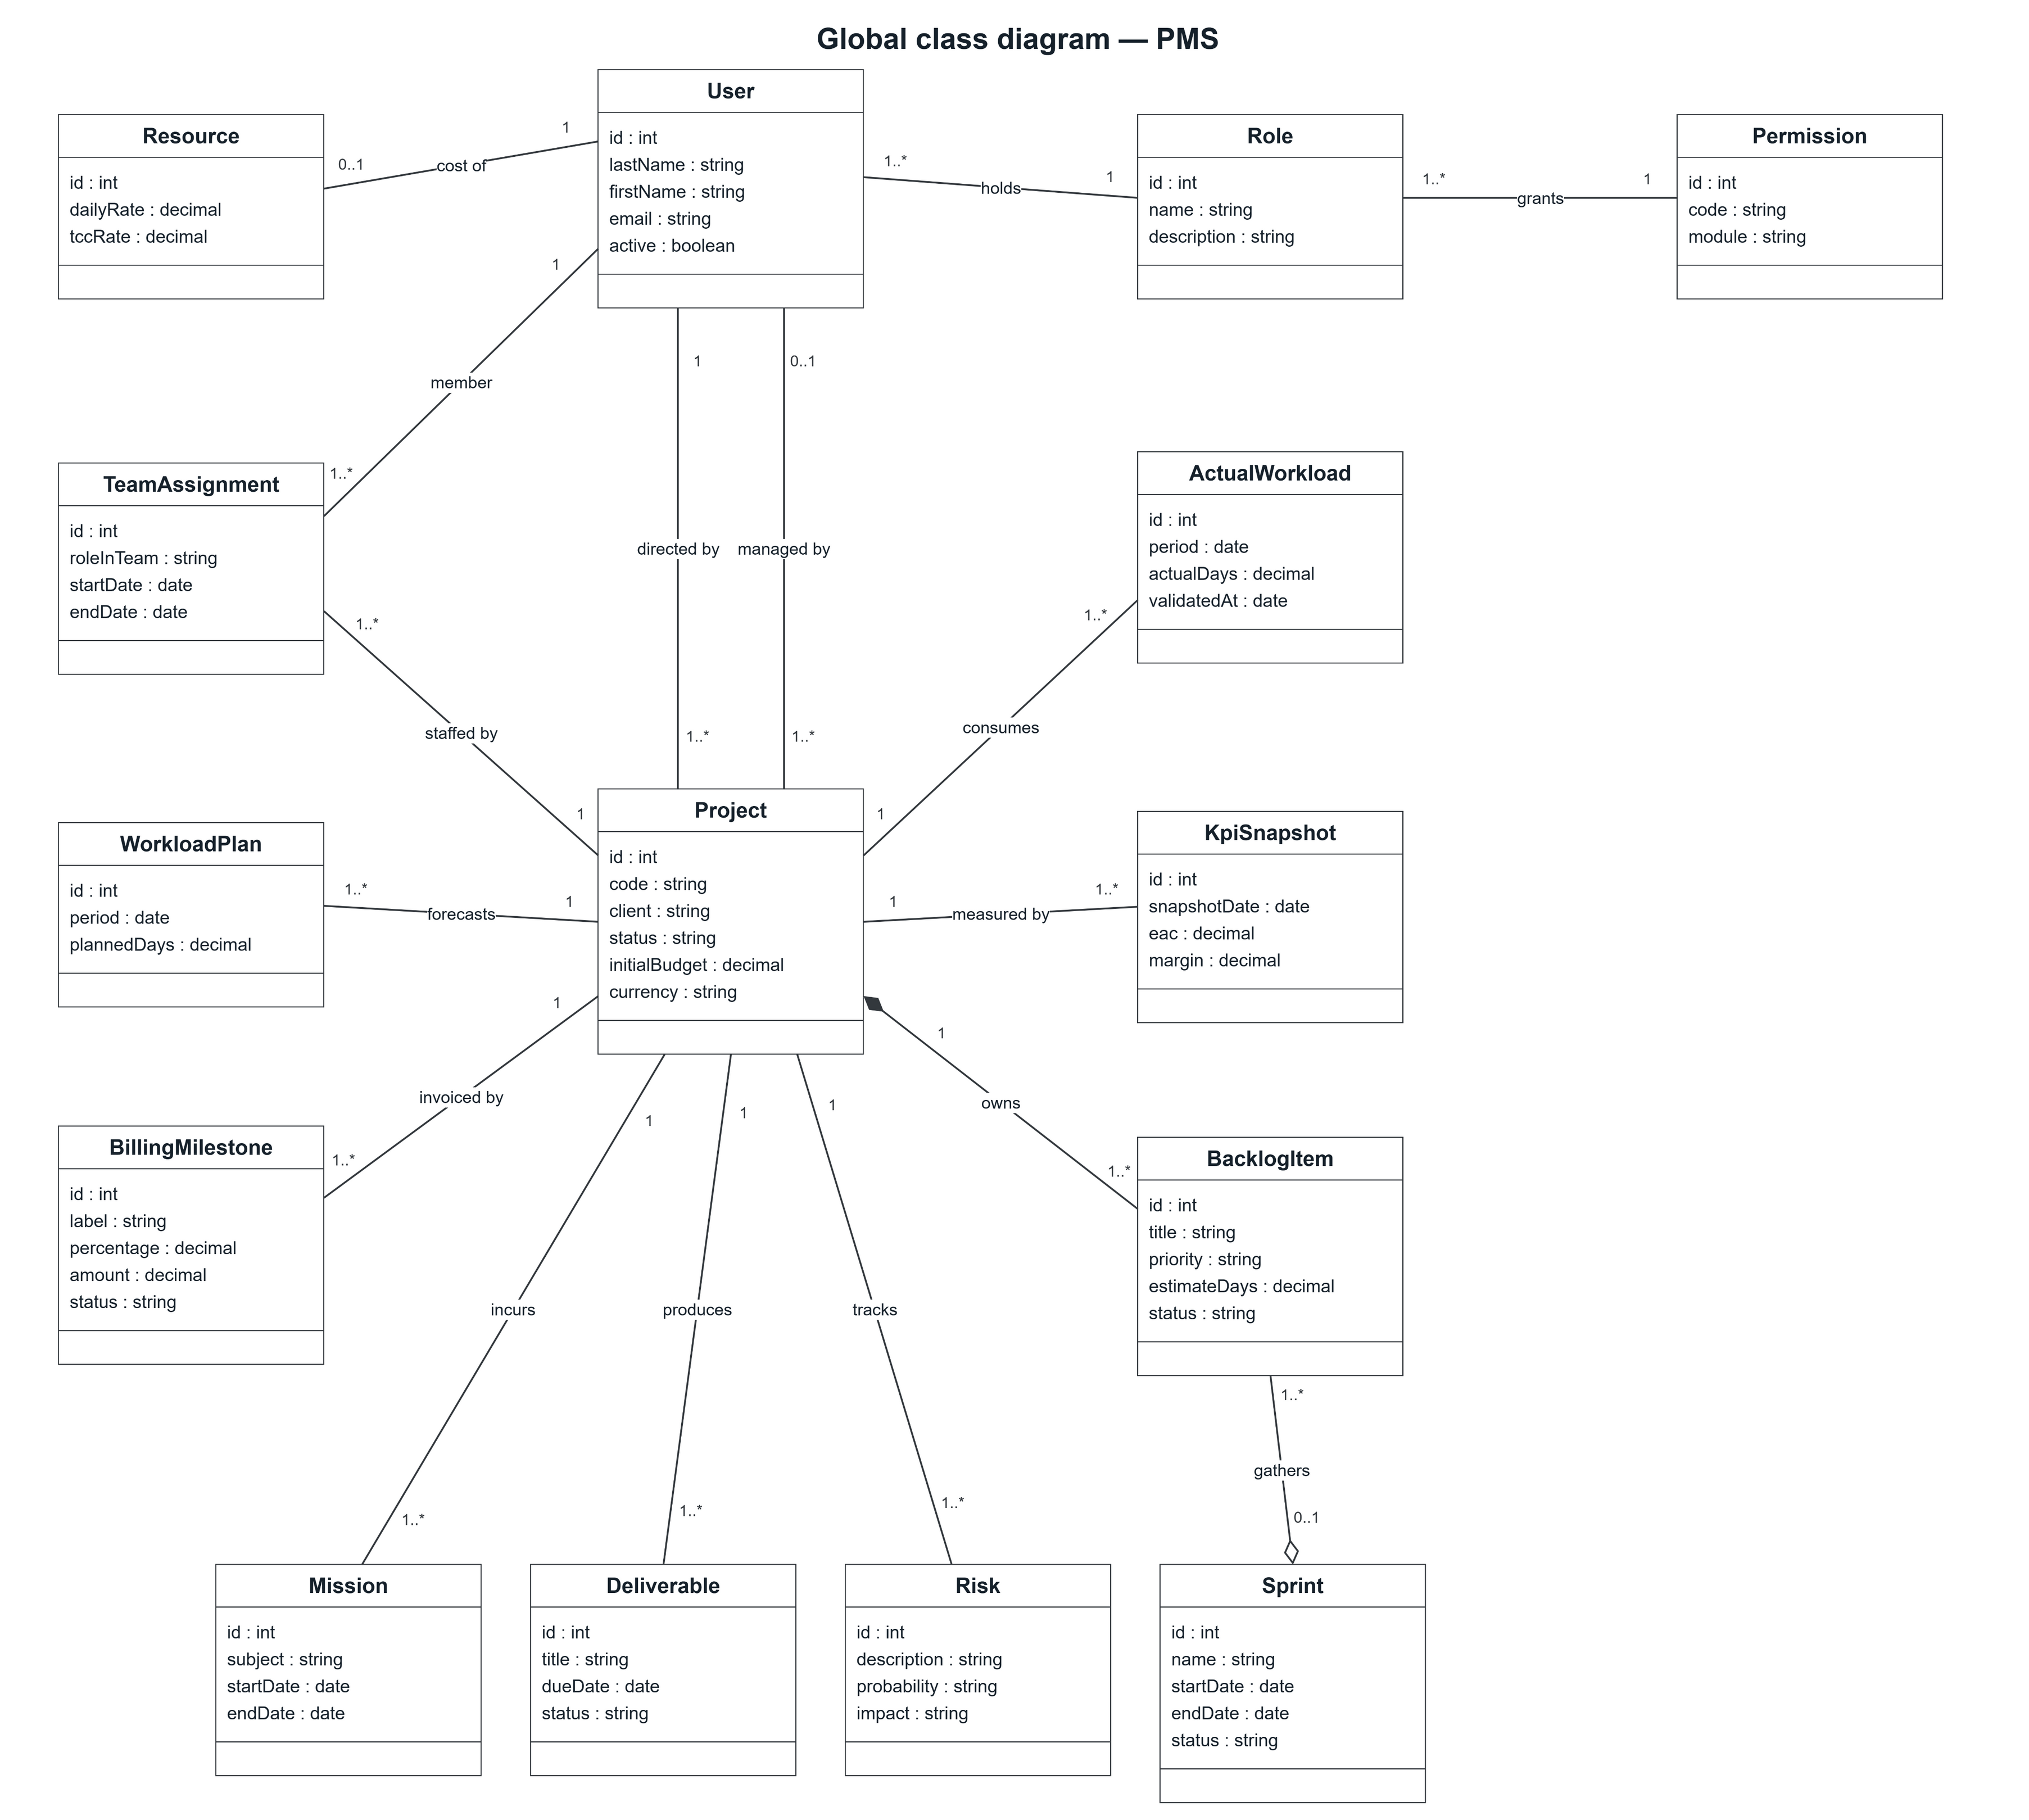
\includegraphics[width=\columnwidth]{img/class_global.png}
  \caption{Domain model --- principal classes and their associations}
  \label{fig:class-global}
\end{figure}

One reading of the diagram deserves to be made explicit, because it is easy to expect the
opposite. The four roles of the platform are not subclasses of \texttt{User}: they are rows of
the \texttt{Role} class. A user holds a role, and a role grants permissions, so the authorization
policy is data that an administrator edits rather than a hierarchy compiled into the application.
Modelling the roles as types would have contradicted that, and would have made every change of
policy a new version of the software.

The diagram stays at the level of the principal classes and their key attributes. Each sub-domain
is detailed by its own class diagram, presented in the sprint that builds it: security in
Sprint~2 (Figure~\ref{fig:class-sec}), projects and teams in Sprint~3, agile planning in
Sprint~5, financial management in Sprint~6, governance in Sprint~7, and the indicator engine in
Sprint~8.

\begin{figure}[H]
  \centering
  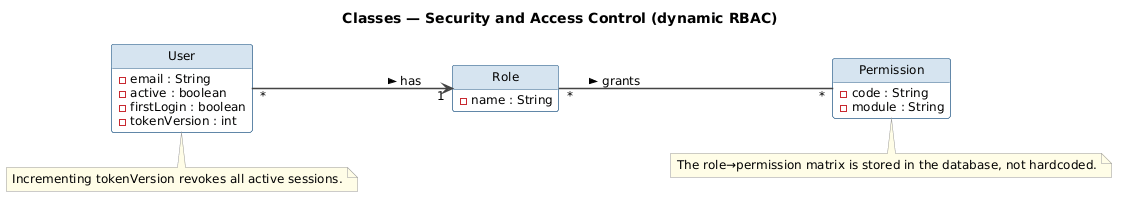
\includegraphics[width=0.75\columnwidth]{img/class_security.png}
  \caption{Class diagram --- security and access control}
  \label{fig:class-sec}
\end{figure}

\section{Database Design}

\subsection{Modelling Conventions}
The schema targets PostgreSQL and follows uniform conventions:

\begin{itemize}
  \item tables in \texttt{snake\_case}, plural; identity primary key \texttt{id};
  \item foreign keys named \texttt{<entity>\_id}; timestamps in \texttt{timestamptz};
  \item amounts stored as \texttt{numeric(18,3)} with an explicit currency column, never as
        floating point, to avoid rounding drift on financial aggregates;
  \item months stored as the \textbf{first day of the month}, making the workload a true time
        series;
  \item enumerations expressed as \texttt{varchar} constrained by \texttt{CHECK};
  \item audit columns and logical deletion on every business table.
\end{itemize}

\subsection{Logical Model}
The core of the schema is the dynamic access control: \texttt{users} references \texttt{roles}, and
\texttt{roles} relates to \texttt{permissions} through the \texttt{role\_permissions} association.
A project references its director and groups its child entities: project manager assignment (a
single active one at a time), team assignments, workload plan, actual workload, billing milestones,
missions, governance registers and KPI snapshots. A resource carries one cost rate per year and may
be linked to a user account.

\begin{longtable}{|m{3.6cm}|m{7.4cm}|m{3.4cm}|}
\hline
\textbf{Domain} & \textbf{Main tables} & \textbf{Module} \\
\hline
\endhead
\endfoot
\endlastfoot
\hline
Security / RBAC & \texttt{users}, \texttt{roles}, \texttt{permissions},
\texttt{role\_permissions} & Authentication \& RBAC \\
\hline
Reference data & \texttt{currencies}, \texttt{exchange\_rates}, \texttt{parameters}, risk scales &
Configuration \\
\hline
Resources & \texttt{resources}, \texttt{tcc} & Cost rate management \\
\hline
Projects & \texttt{projects}, \texttt{project\_manager\_assignments} & Project management \\
\hline
Teams & \texttt{team\_assignments}, \texttt{stakeholders} & Teams \\
\hline
Workload & \texttt{workload\_plan}, \texttt{actual\_workload} & Planning / Actuals \\
\hline
Billing & \texttt{billing\_milestones}, \texttt{payments}, \texttt{avenants} & Billing \\
\hline
Missions & \texttt{missions} & Mission management \\
\hline
Governance & \texttt{risks}, \texttt{deliverables}, \texttt{change\_requests}, \texttt{actions} &
Governance \\
\hline
Indicators & \texttt{kpi\_snapshots} & KPI \& Reporting \\
\hline
\caption{Catalogue of entities by domain}
\label{tab:entities}
\end{longtable}

\subsection{Monthly Time Series and Indicator Snapshots}
The Excel workbook is a resource~$\times$~month grid. Rather than reproducing twenty-five month
columns, the model is \textbf{normalised}: one row per (project, resource, month) in
\texttt{workload\_plan} and \texttt{actual\_workload}. Adding a month becomes inserting a row rather
than altering the schema.

The \texttt{kpi\_snapshots} table stores one snapshot per (project, month), which yields both the
history needed for evolution curves and fast reads for dashboards. It deliberately separates the
\textbf{labour cost} (man-days $\times$ cost rate) from \textbf{other costs} (missions and
expenses), the total aggregating the two. The original workbook blurred that distinction, which
matters when analysing why a project drifts.

\subsection{Reference Data and Migration Strategy}
A seed dataset creates the four roles, the full permission catalogue, the default role--permission
matrix, the currencies, the business parameters, the risk scales and a bootstrap administrator.

The schema is managed exclusively by \textbf{Flyway} versioned SQL migrations, with the ORM in
\texttt{validate} mode: the entities must match the schema, never generate it. The migrations
constitute the living documentation of the database and make every schema change reviewable and
reproducible.

\section{Deployment Architecture}
Figure~\ref{fig:deploy} shows the target deployment: a browser running the single-page
application, an application server exposing the REST API, and a database server. The whole
platform is a single deployable artefact, consistent with the modular monolith decision.

\begin{figure}[H]
  \centering
  
\includegraphics[width=0.55\columnwidth]{img/deployment_diagram.png}
  \caption{Deployment architecture}
  \label{fig:deploy}
\end{figure}

\section{Technical Environment}
Every technology below was chosen against the same two constraints: a single developer with eight
months, and a platform whose value lies in financial correctness rather than in scale. That
combination consistently favours mature, well-documented tools with a short path from decision to
working code, over newer ones that would have to be learned first.

\subsection{Backend}

\begin{longtable}{|m{1.9cm}|m{2.5cm}|m{10.0cm}|}
\hline
\textbf{} & \textbf{Technology} & \textbf{What it is, and why it was chosen} \\
\hline
\centering
\includegraphics[width=1.65cm,height=1.05cm,keepaspectratio]{img/logo_java.png} & Java~21 &
A statically typed, object-oriented language running on a virtual machine. Version~21 is a
long-term-support release, so the platform rests on a version that will still be maintained well
after the internship. It is also the language named by the assigned subject. \\
\hline
\centering
\includegraphics[width=1.65cm,height=1.05cm,keepaspectratio]{img/logo_springboot.png} & Spring Boot~3.3 &
A framework that turns a Java application into a self-contained, runnable server with its
dependencies already wired. It was chosen because it removes almost all configuration work:
persistence, security, validation and the REST layer are declared rather than assembled, which is
what makes ten sprints of business features possible for one developer. \\
\hline
\centering
\includegraphics[width=1.65cm,height=1.05cm,keepaspectratio]{img/logo_springsecurity.png} & Spring Security &
The security layer of the same framework, handling authentication and authorization. It was chosen
because it supports exactly the model this platform needs: a check expressed as a permission the
caller must hold, evaluated on the method rather than on the route, which is what allows the
authorization policy to live in the database instead of in the code. \\
\hline
\centering
\includegraphics[width=1.65cm,height=1.05cm,keepaspectratio]{img/logo_hibernate.png} & Hibernate (JPA) &
The object-relational mapper that translates between Java objects and database rows. It was chosen
for one property in particular: it can be told to \emph{validate} the schema at startup instead of
generating it, so a divergence between the code and the database stops the application immediately
rather than corrupting data later. \\
\hline
 & MapStruct &
A code generator that writes the conversions between entities and the objects returned by the API.
It was chosen so that persistence structures are never exposed directly by the REST layer, without
paying for that separation in hand-written boilerplate. \\
\hline
\caption{Backend technologies}
\label{tab:tech-backend}
\end{longtable}

\subsection{Database}

\begin{longtable}{|m{1.9cm}|m{2.5cm}|m{10.0cm}|}
\hline
\textbf{} & \textbf{Technology} & \textbf{What it is, and why it was chosen} \\
\hline
\centering
\includegraphics[width=1.65cm,height=1.05cm,keepaspectratio]{img/logo_postgresql.png} & PostgreSQL~17 &
An open-source relational database. It was chosen over a document store because the domain is
relational by nature: a project, its team, its milestones and its monthly workload are joined
constantly. Its exact decimal type also matters here, since financial totals computed in floating
point drift by fractions of a dinar and a report that does not balance is worthless. \\
\hline
\centering
\includegraphics[width=1.65cm,height=1.05cm,keepaspectratio]{img/logo_flyway.png} & Flyway &
A schema migration tool: every change to the database is a numbered, versioned script rather than a
manual operation. It was chosen because it makes the schema reproducible and reviewable, and
because the twenty-seven migrations it holds are the living documentation of how the schema
reached its present shape. \\
\hline
\caption{Database technologies}
\label{tab:tech-database}
\end{longtable}

\subsection{Frontend}

\begin{longtable}{|m{1.9cm}|m{2.5cm}|m{10.0cm}|}
\hline
\textbf{} & \textbf{Technology} & \textbf{What it is, and why it was chosen} \\
\hline
\centering
\includegraphics[width=1.65cm,height=1.05cm,keepaspectratio]{img/logo_angular.png} & Angular~21 &
A framework for building single-page applications: the browser loads the application once and then
exchanges only data with the server. It was chosen because it is opinionated. Routing, forms, HTTP
and internationalisation all come from the framework, so a single developer spends the time on
screens rather than on choosing and gluing libraries. It is also the framework named by the
assigned subject. \\
\hline
\centering
\includegraphics[width=1.65cm,height=1.05cm,keepaspectratio]{img/logo_typescript.png} & TypeScript &
JavaScript with static types. It was chosen for the same reason the backend is typed: the platform
manipulates money, and a field that silently changes shape between the API and the screen is a
class of error worth eliminating at compile time. \\
\hline
\caption{Frontend technologies}
\label{tab:tech-frontend}
\end{longtable}

\subsection{Tooling}

\begin{longtable}{|m{1.9cm}|m{2.5cm}|m{10.0cm}|}
\hline
\textbf{} & \textbf{Tool} & \textbf{What it is, and why it was chosen} \\
\hline
\centering
\includegraphics[width=1.65cm,height=1.05cm,keepaspectratio]{img/logo_maven.png} & Maven &
The build tool for the backend: it resolves dependencies, compiles, runs the tests and produces the
executable archive. Chosen because it is the default in the Spring ecosystem, so every example in
the documentation applies without translation. \\
\hline
\centering
\includegraphics[width=1.65cm,height=1.05cm,keepaspectratio]{img/logo_git.png} & Git &
Distributed version control. Chosen for the ordinary reason: it keeps the history of the work and
makes any change reversible. The repository is hosted privately, since the platform contains the
company's financial logic. \\
\hline
\centering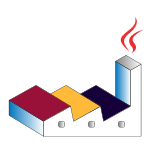
\includegraphics[width=1.65cm,height=1.05cm,keepaspectratio]{img/logo_plantuml.png} & PlantUML &
A tool that renders UML diagrams from a plain-text description. It was chosen so that the diagrams
of this report are versioned as source next to the code: a diagram that is a text file is reviewed,
diffed and corrected like anything else, whereas an exported image quietly goes out of date. \\
\hline
\centering
\includegraphics[width=1.65cm,height=1.05cm,keepaspectratio]{img/logo_lucidchart.png} & Lucidchart &
A diagramming application used for the global class diagram of Figure~\ref{fig:class-global}. That
one diagram is the map of the whole domain and needed to be laid out by hand, grouping the classes
as a reader thinks about them rather than as an automatic layout engine places them, which is what
a direct-manipulation editor does better than a text-driven one. \\
\hline
\caption{Development and modelling tools}
\label{tab:tech-tooling}
\end{longtable}

Containerization arrived later, in Sprint~10, and is presented there
(Section~\ref{sec:sprint10}) rather than here, because it was a decision the project revisited
rather than one taken at the outset.

\section*{Conclusion}
The architecture retained, a three-tier modular monolith with dynamic authorization, a hybrid
indicator engine and a normalised time-series schema, answers the requirements of Chapter~2
while remaining proportionate to the scale of the target deployment. These decisions are now
applied: the following chapters present the progressive construction of the platform, release by
release and sprint by sprint.

        \clearpage

        \chapter{Authentication and Access Control}

\section*{Introduction}
This chapter presents the first release of the PMS platform. Its purpose is to make the application
usable and secure before any business functionality is built on top of it. It opens with the
preparation phase, six weeks of study that preceded the first line of production code, and then
gathers two sprints: Sprint~1 establishes the technical foundation and the authentication chain,
Sprint~2 delivers the dynamic authorization model together with the management of users and
resources.

At the end of this release the platform authenticates its users, applies a configurable
authorization policy, and holds the reference data, that is users, resources and cost rates, which
the operational modules of the next release consume.

% =====================================================================
\section{Release 1 backlog}
The first release realises the seven user stories of the product backlog
(Table~\ref{tab:backlog}) that concern access to the platform. Because the author is the sole
developer, each story is expanded into the technical work it required.

\begin{longtable}{|m{1.5cm}|m{6.8cm}|m{5.2cm}|m{1.4cm}|}
\hline
\textbf{Story} & \textbf{Need} & \textbf{Technical work} & \textbf{Sprint} \\
\hline
\endhead
\endfoot
\endlastfoot
\hline
US-01 & Sign in with an e-mail and a password & Authentication service, BCrypt verification, JWT
issuance signed with HMAC-SHA512, refresh cookie, token rotation & 1 \\
\hline
US-02 & Be forced to change an imposed password on first login & \texttt{first\_login} flag,
dedicated filter restricting the token to the password-change endpoint & 1 \\
\hline
US-03 & Revoke a user's sessions immediately & Token version persisted per user, embedded in each
token and compared on every request & 1 \\
\hline
US-04 & Assign permissions to roles without redeploying & \texttt{roles}, \texttt{permissions} and
\texttt{role\_permissions} tables, permissions carried in the token and converted into Spring
Security authorities & 2 \\
\hline
US-05 & See only the menu entries the account is entitled to & Context endpoint returning the held
permissions, navigation built from that response & 2 \\
\hline
US-06 & Create, modify and deactivate user accounts & User module, creation with a temporary
password, activation state, role assignment & 2 \\
\hline
US-07 & Record resources and their yearly cost rate & Resource entity separate from the account,
loaded cost rate stored per resource and per year & 2 \\
\hline
\caption{Backlog of release 1}
\label{tab:backlog-r1}
\end{longtable}

% =====================================================================
\section{Preparation phase}
The release opens with six weeks that produced no production code. They ran from 5~January to
13~February and are listed as such in the schedule of Chapter~2
(Table~\ref{tab:schedule}). Their purpose was to arrive at the first sprint already knowing what
had to be built, on which architecture, and what it should look like.

\subsection{What the phase produced}
Four deliverables came out of it, each of which is presented in full elsewhere in this report and
only summarised here.

\begin{itemize}
  \item \textbf{The reading of the existing instrument.} The project review workbook was opened
        sheet by sheet, its formulas traced, and its business rules written down. This is the
        analysis of Chapter~1, and it is the reason the platform reproduces the company's financial
        model rather than an approximation of it.
  \item \textbf{The requirements and the product backlog.} The rules extracted from the workbook
        were turned into actors, functional and non-functional requirements, and twenty-five user
        stories distributed across four releases. This is Chapter~2.
  \item \textbf{The architecture and the technical stack.} The modular monolith, the dynamic
        authorization model, the hybrid indicator engine and the relational schema were decided
        before any of them was written. This is Chapter~3.
  \item \textbf{The interface models.} Screen models were produced for the main workflows, so that
        the sprints could be spent implementing an agreed interface rather than inventing one under
        time pressure. These models are the subject of the rest of this section.
\end{itemize}

\subsection{Interface models}
The models were produced with \textbf{Google Stitch}, a generative interface design tool: each
screen is described in natural language and the tool returns a working layout that can then be
refined. It was chosen for a reason specific to this project, which had a single developer and no
designer. Producing a credible screen in minutes rather than days made it affordable to explore
several arrangements of the same information, and to discard the ones that did not work before any
of them cost a sprint.

Two things should be said plainly about these models. They carry a provisional product name,
\emph{ProjectControl}, and amounts in euros, because they were exploratory sketches rather than
specifications; the delivered platform is named PMS and reports in Tunisian dinars. And they are
models of \emph{layout and information hierarchy} only: no model describes a permission, a
computation or a state transition, all of which come from the analysis rather than from the design
tool.

\subsubsection{Sign-in}
The entry point of the platform was the first screen modelled, because it is the only one every
user sees and the only one seen before any authorization applies.

\begin{figure}[H]
  \centering
  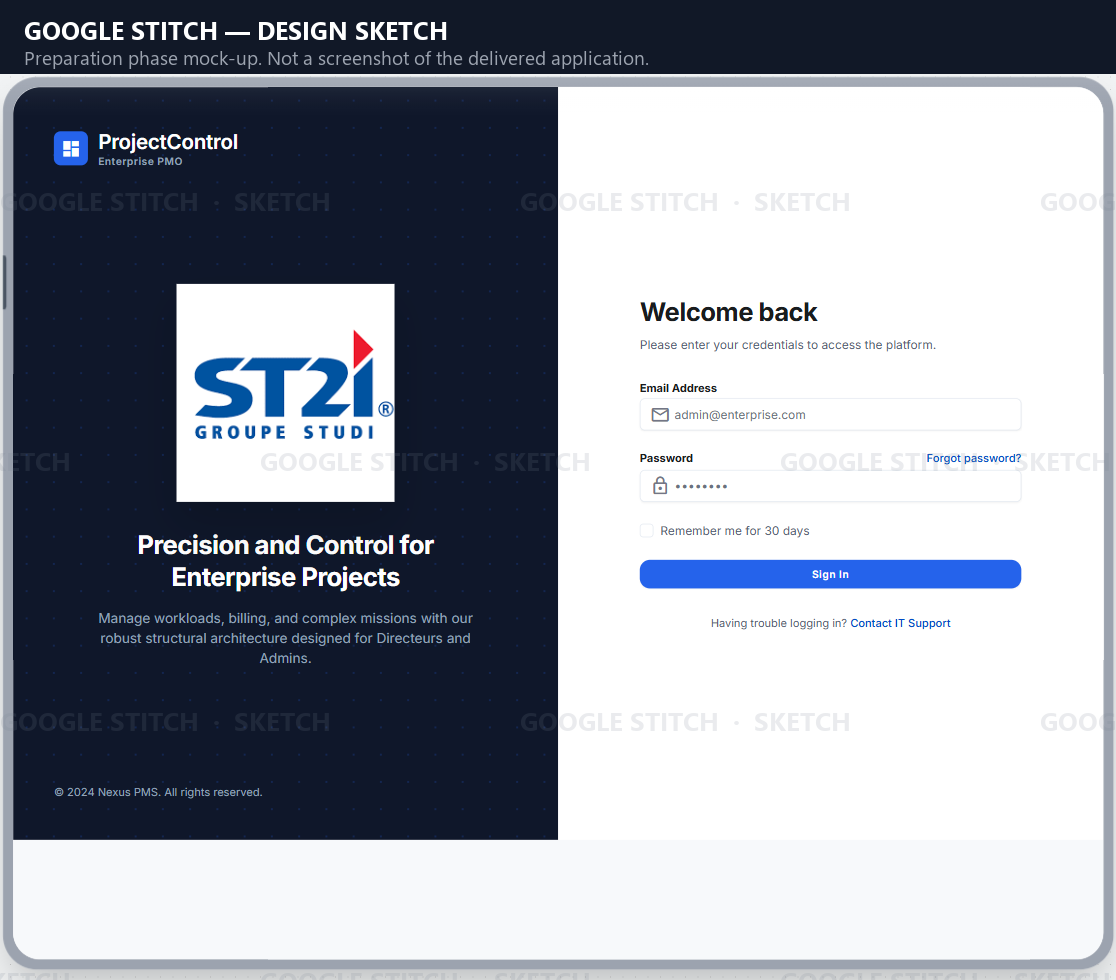
\includegraphics[width=0.88\columnwidth]{img/mk_login.png}
  \caption{Interface model --- sign-in screen}
  \label{fig:mk-login}
\end{figure}

\subsubsection{Steering screens}
The director reads the portfolio; the project manager reads one project in depth. The models
separated those two readings from the start, which is what later became the portfolio dashboard and
the per-project indicator board of Sprint~8.

\begin{figure}[H]
  \centering
  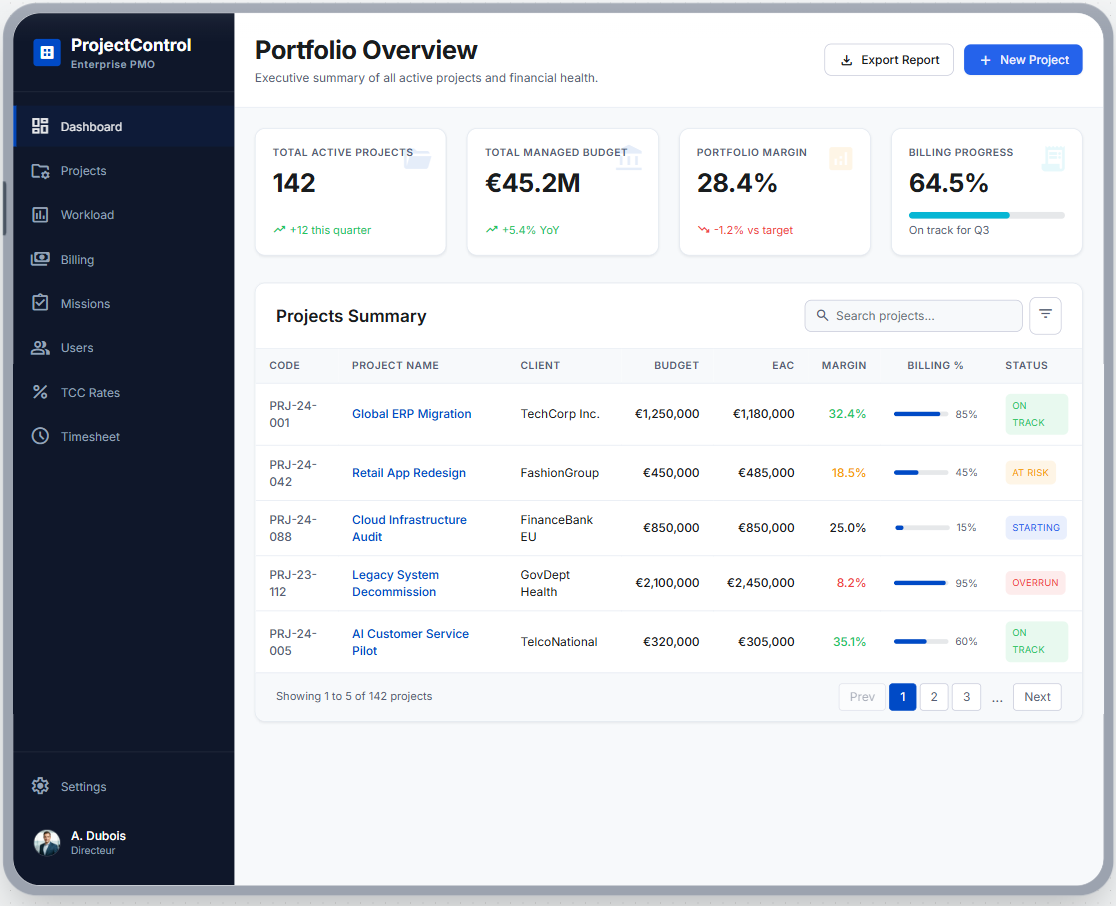
\includegraphics[width=0.88\columnwidth]{img/mk_portfolio.png}
  \caption{Interface model --- portfolio overview for the director}
  \label{fig:mk-portfolio}
\end{figure}

\begin{figure}[H]
  \centering
  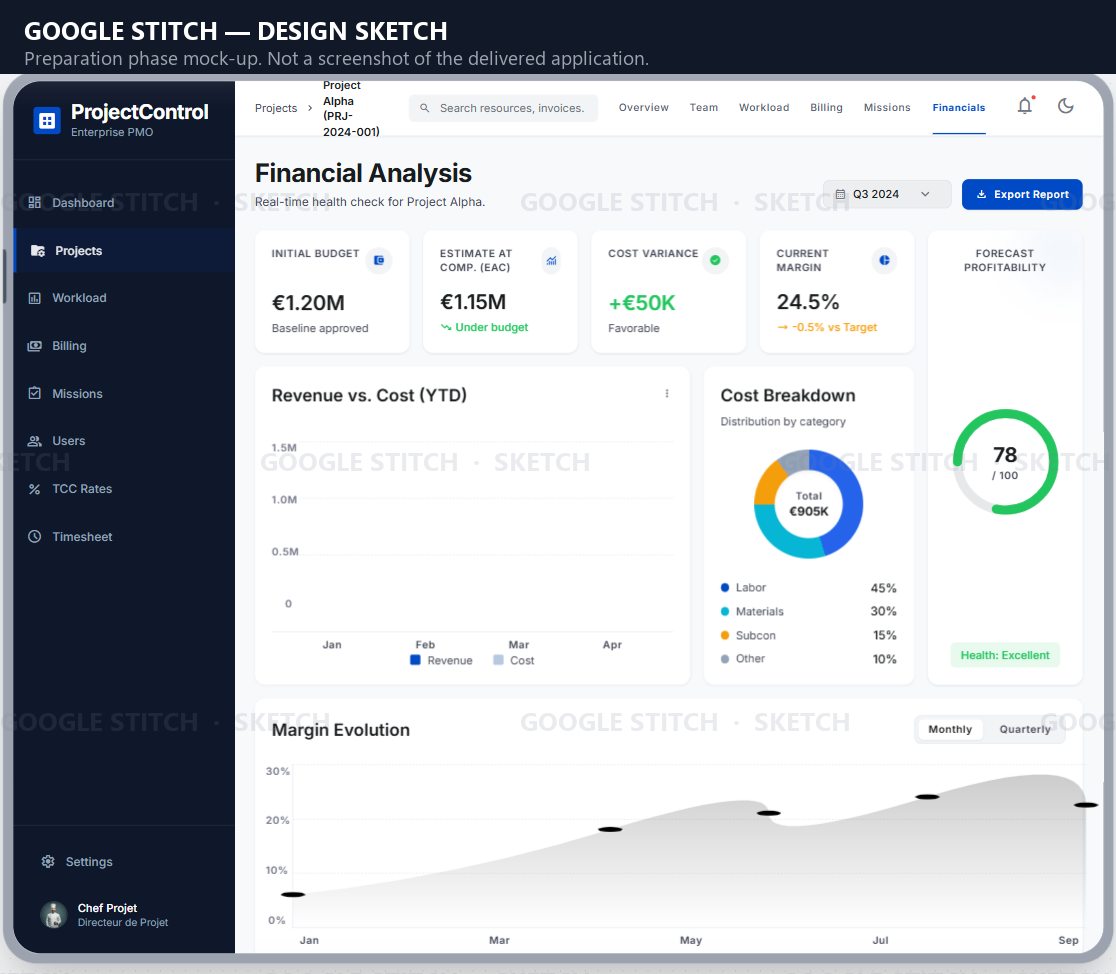
\includegraphics[width=0.88\columnwidth]{img/mk_financial.png}
  \caption{Interface model --- financial analysis of a single project}
  \label{fig:mk-financial}
\end{figure}

\subsubsection{Operational screens}
The workload matrix and the billing timeline are the two screens that carry the most business
logic, and both were modelled before being built.

\begin{figure}[H]
  \centering
  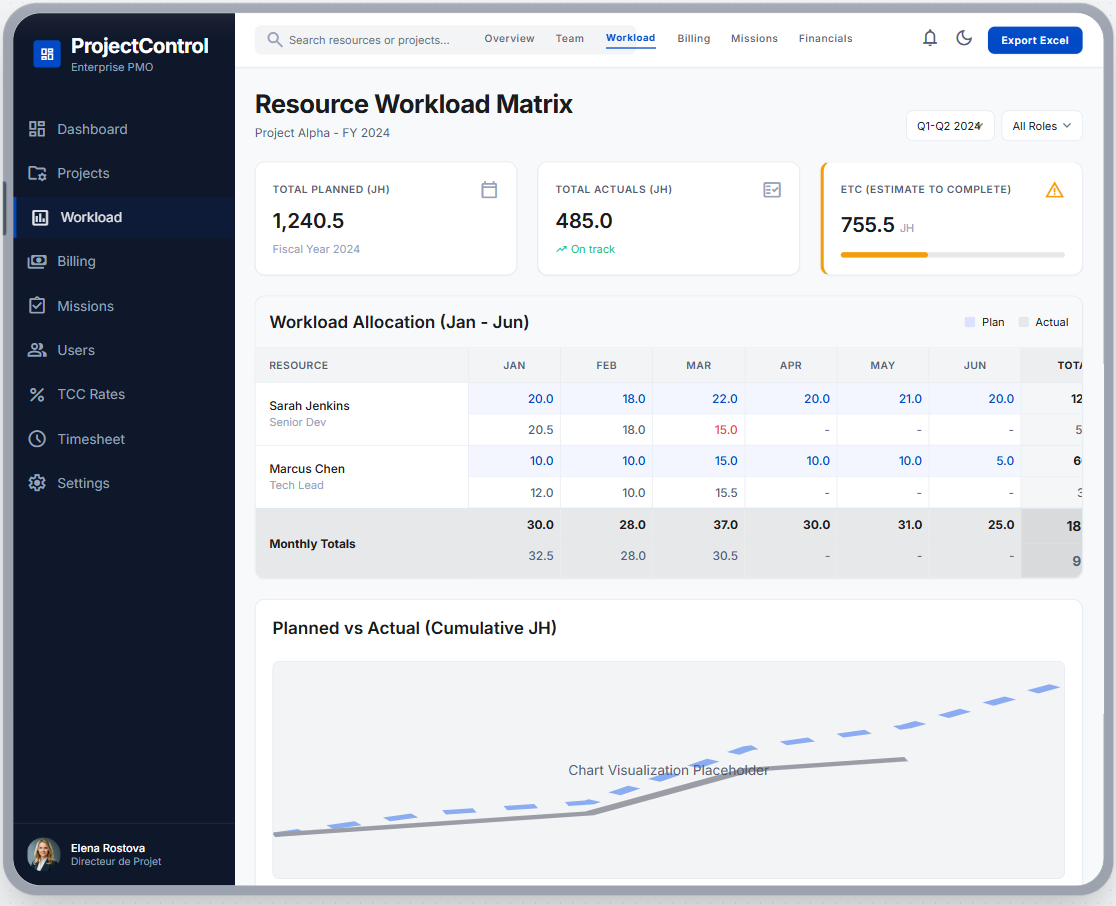
\includegraphics[width=0.88\columnwidth]{img/mk_workload.png}
  \caption{Interface model --- resource workload matrix, planned against actual}
  \label{fig:mk-workload}
\end{figure}

\begin{figure}[H]
  \centering
  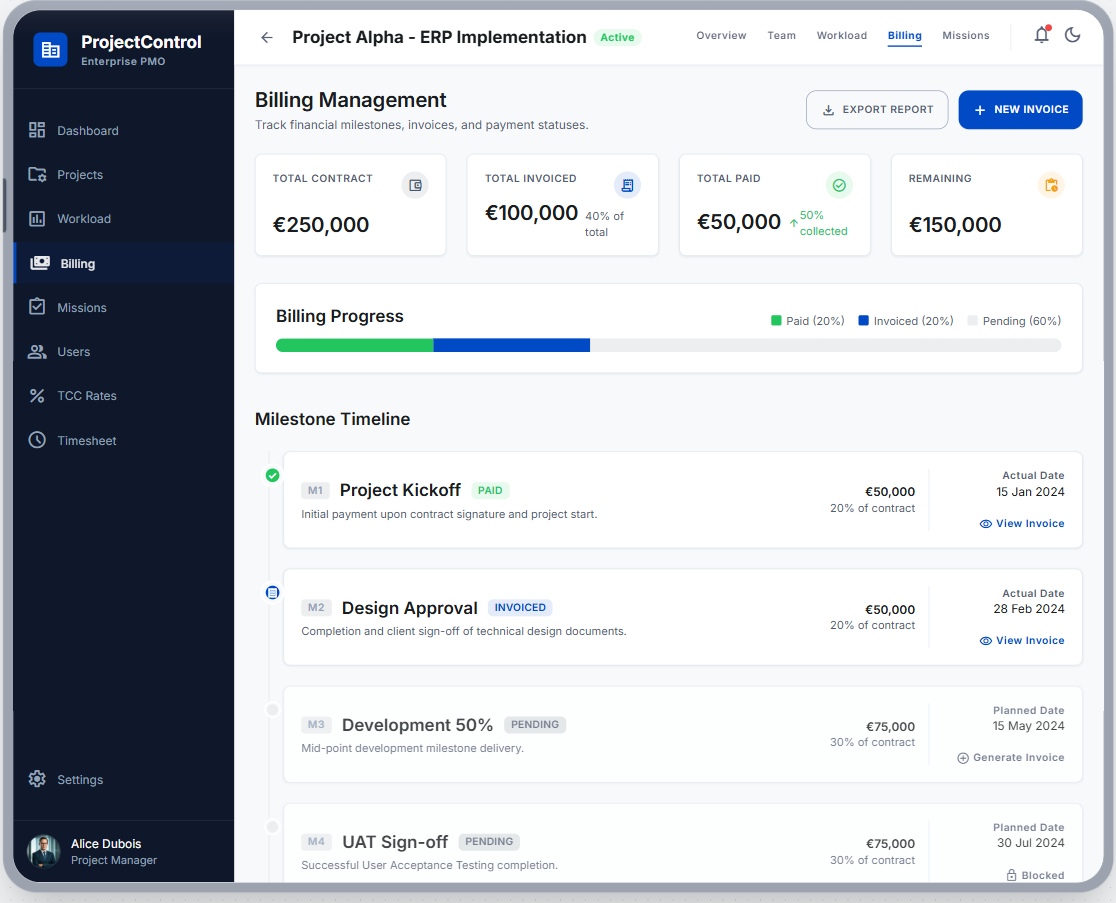
\includegraphics[width=0.88\columnwidth]{img/mk_billing.png}
  \caption{Interface model --- billing milestones and their progress}
  \label{fig:mk-billing}
\end{figure}

\subsubsection{Screens of the restricted roles}
Modelling the developer and administrator views early was what made the consequence of the
authorization model visible before it was implemented: a role that holds few permissions does not
get a reduced version of the same screen, it gets a different and much shorter menu.

\begin{figure}[H]
  \centering
  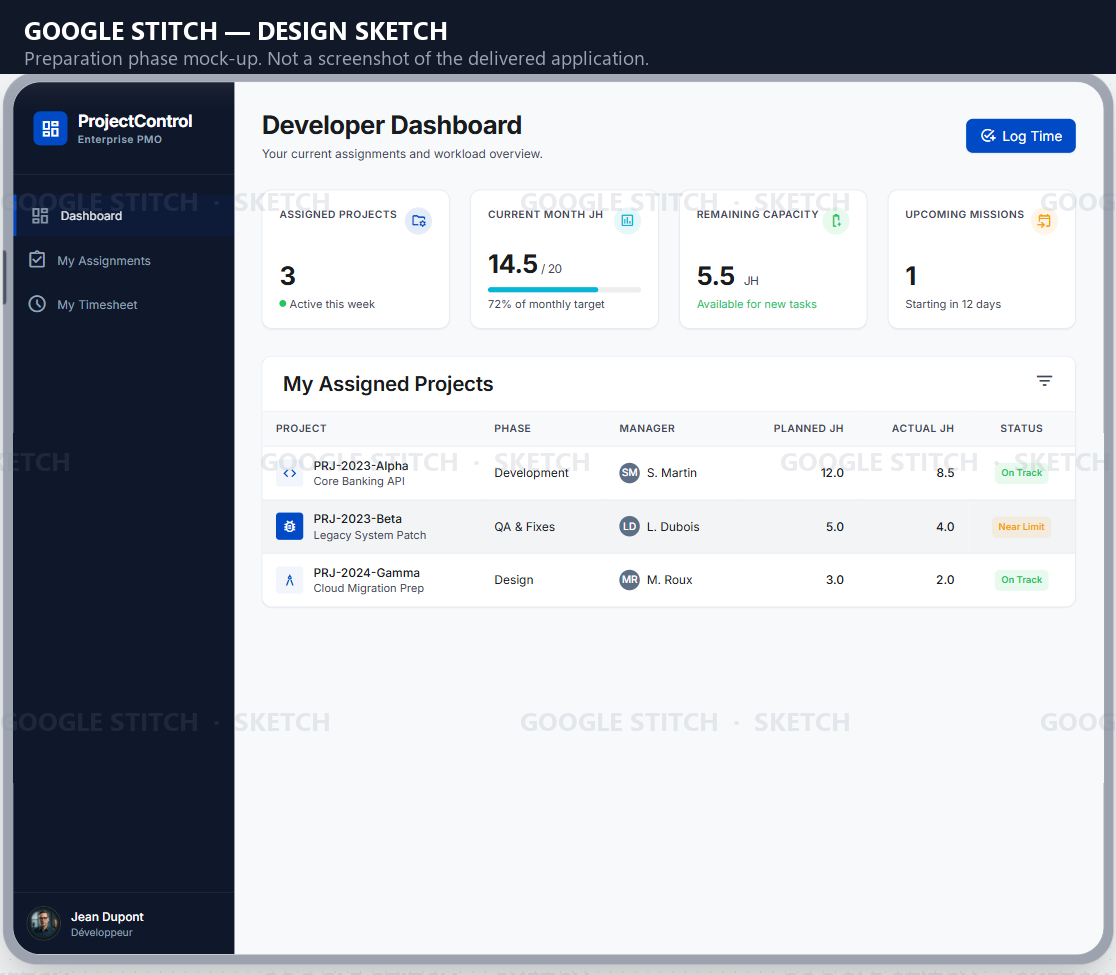
\includegraphics[width=0.88\columnwidth]{img/mk_developer.png}
  \caption{Interface model --- developer workspace, reduced to assignments and time entry}
  \label{fig:mk-developer}
\end{figure}

\begin{figure}[H]
  \centering
  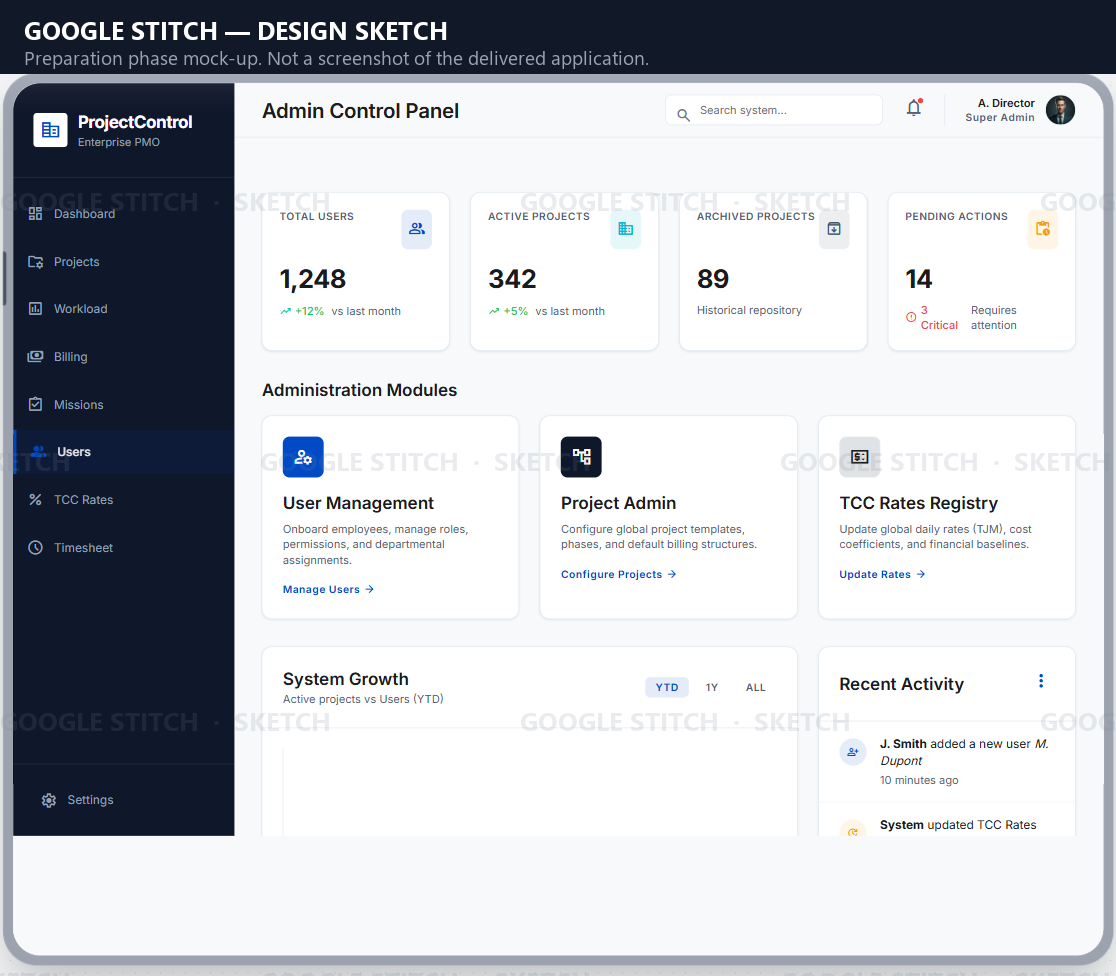
\includegraphics[width=0.88\columnwidth]{img/mk_admin.png}
  \caption{Interface model --- administration panel}
  \label{fig:mk-admin}
\end{figure}

\subsection{From the models to the delivered interface}
Table~\ref{tab:model-traceability} follows each model through to the screen that was actually
delivered, and records where the two diverge. The divergences are the useful part: they are the
places where implementation taught something the model could not.

\begin{longtable}{|m{3.5cm}|m{3.4cm}|m{7.0cm}|}
\hline
\textbf{Model} & \textbf{Delivered screen} & \textbf{What changed, and why} \\
\hline
\endhead
\endfoot
\endlastfoot
\hline
Sign-in (Fig.~\ref{fig:mk-login}) & Fig.~\ref{fig:ui-login} & Kept almost unchanged. The forced
password change on first login was added, because it comes from a security requirement the model
did not express. \\
\hline
Portfolio overview (Fig.~\ref{fig:mk-portfolio}) & Fig.~\ref{fig:ui-portfolio} & The summary tiles
survived. The flat project table became a ranking by margin with a portfolio health bar, because
a director scanning eighty projects needs the worst ones first, not the newest. \\
\hline
Financial analysis (Fig.~\ref{fig:mk-financial}) & Fig.~\ref{fig:ui-kpi} & The indicator set was
replaced by the one the workbook actually defines: EAC, ETC, accrued income and drift in man-days,
rather than the generic cost breakdown the model proposed. \\
\hline
Workload matrix (Fig.~\ref{fig:mk-workload}) & Fig.~\ref{fig:ui-workload} & Confirmed. The
planned-against-actual matrix by resource and by month is the arrangement the workbook already
used, and the model made it visible early enough to build it once. \\
\hline
Billing (Fig.~\ref{fig:mk-billing}) & Fig.~\ref{fig:ui-billing} & The vertical timeline became a
table. A milestone is compared with its neighbours far more often than it is read on its own, and a
table compares better than a timeline. \\
\hline
Developer workspace (Fig.~\ref{fig:mk-developer}) & Fig.~\ref{fig:ui-dev-dashboard} & Confirmed in
shape, and made a consequence of the permission model rather than a separate screen: the menu is
built from the permissions the account holds. \\
\hline
Administration (Fig.~\ref{fig:mk-admin}) & Figs.~\ref{fig:ui-users} and~\ref{fig:ui-perm-catalogue}
& Split in two. The single panel of the model hid the distinction the platform rests on, between
managing accounts and editing the authorization policy. \\
\hline
\caption{From the interface models to the delivered screens}
\label{tab:model-traceability}
\end{longtable}

The phase closed with the development environment in place: the repository, the database, the
migration tool and the build, so that the first sprint began with a running, empty application
rather than with its installation.

% =====================================================================
\section{Sprint 1 --- Authentication and technical foundation}

\subsection{Sprint 1 use case diagram}
The sprint covers the three use cases that every user must traverse before reaching a business
screen: authenticating, changing an imposed password, and terminating a session. Every other use
case of the platform includes authentication, which is why this sprint precedes all the others.

\begin{figure}[H]
  \centering
  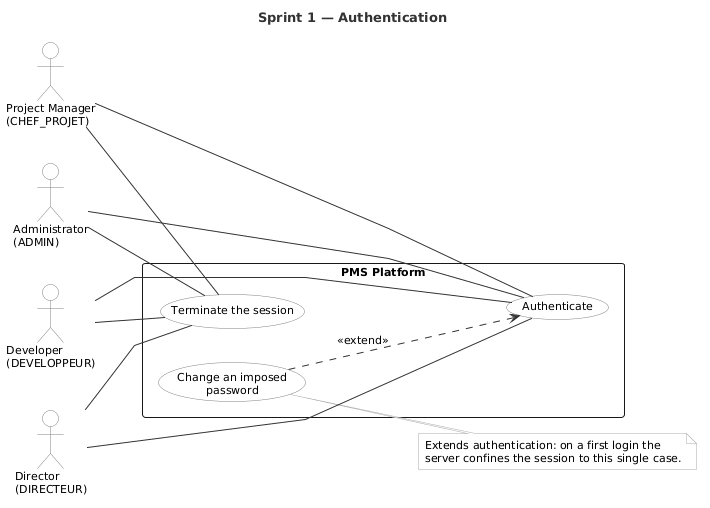
\includegraphics[width=0.75\columnwidth]{img/uc_sprint1.png}
  \caption{Use case diagram of sprint 1}
  \label{fig:uc-s1}
\end{figure}

\subsection{Sprint 1 analysis and design}

\subsubsection{Sequence of the ``Authenticate'' use case}
The nominal scenario involves the browser, the authentication controller, the authentication
service, the token service and the user repository. It shows where the password is verified, where
the two tokens are produced, and why only one of them is written to a cookie.

\begin{figure}[H]
  \centering
  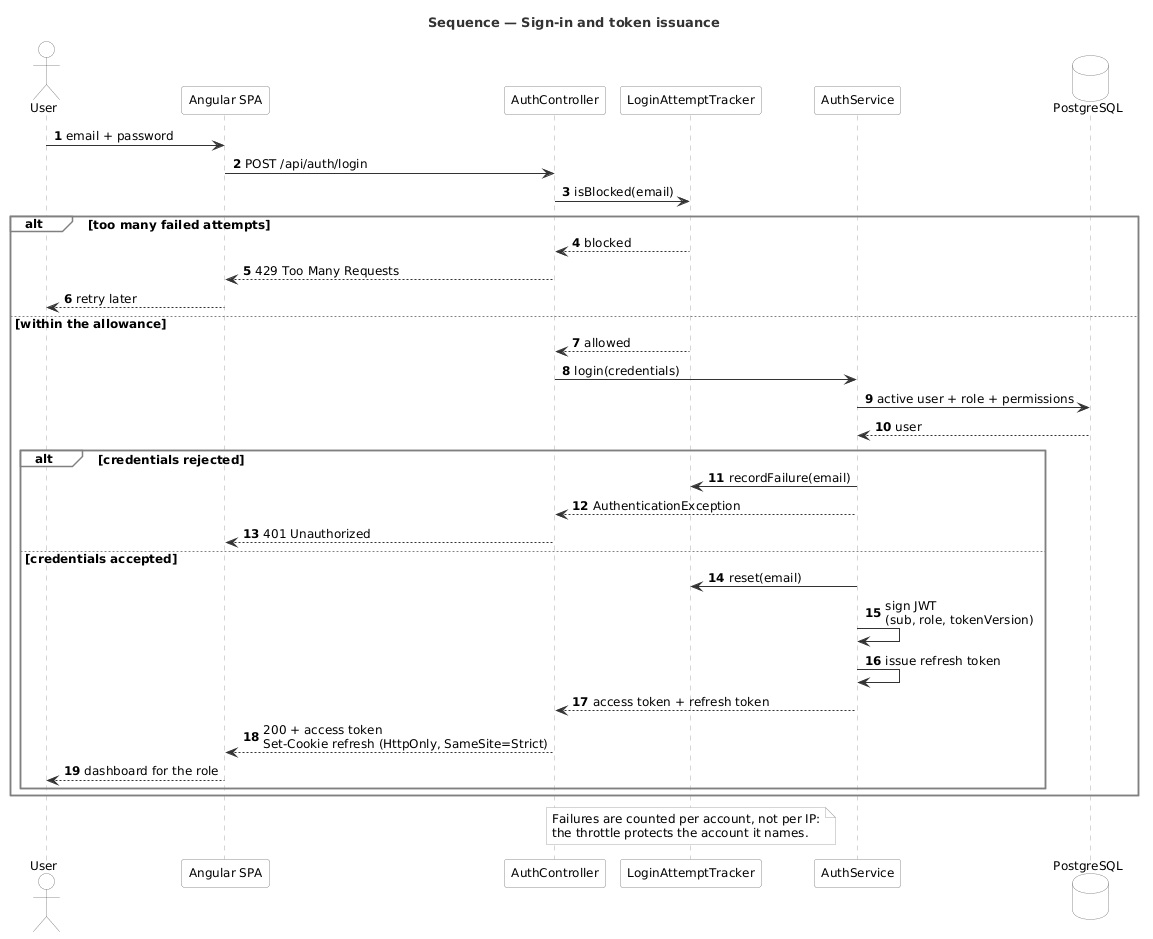
\includegraphics[width=0.95\columnwidth]{img/seq_s1_login.png}
  \caption{Sequence diagram of the ``Authenticate'' use case}
  \label{fig:seq-s1-login}
\end{figure}

\subsubsection{Sequence of the ``Change the password on first login'' use case}
An account created by the administrator carries a temporary password. The scenario shows how the
token issued at the first connection is restricted, how any business call is refused while the flag
remains set, and how a full token is issued once the password has been changed.

\begin{figure}[H]
  \centering
  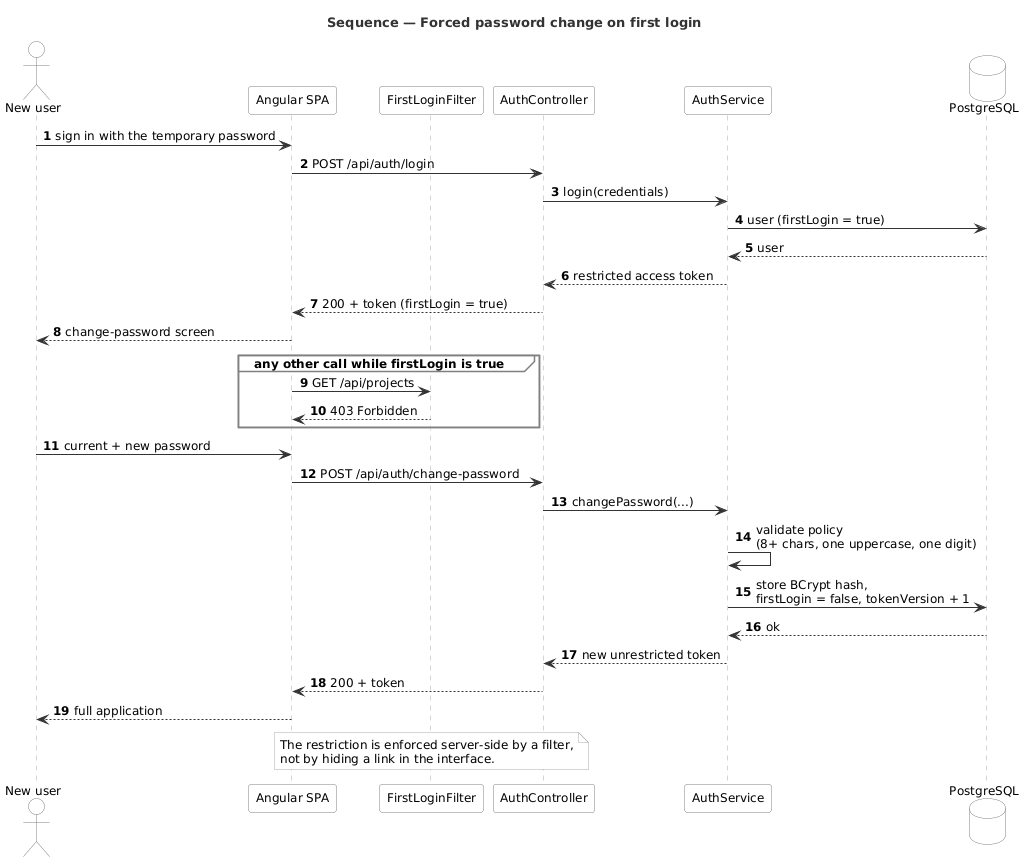
\includegraphics[width=0.95\columnwidth]{img/seq_s1_first_login.png}
  \caption{Sequence diagram of the ``Change the password on first login'' use case}
  \label{fig:seq-s1-first}
\end{figure}

\subsubsection{Sequence of the ``Revoke a session'' use case}
Revocation is the scenario that justifies the design of the token. It shows the increment of the
version, the invalidation of the cache entry, and the rejection of a request presenting a token
issued before the increment.

\begin{figure}[H]
  \centering
  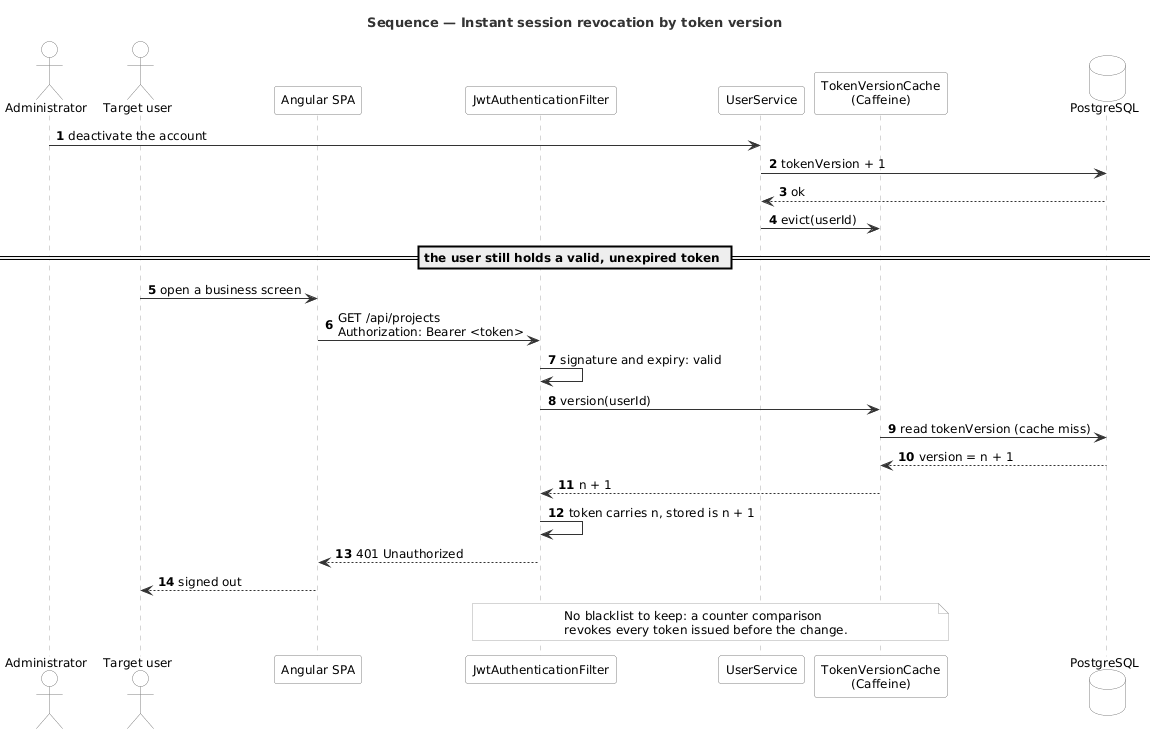
\includegraphics[width=0.95\columnwidth]{img/seq_s1_revoke.png}
  \caption{Sequence diagram of the ``Revoke a session'' use case}
  \label{fig:seq-s1-revoke}
\end{figure}

\subsubsection{Design decisions}
Three decisions taken in this sprint constrain the whole platform and are therefore justified here
rather than in the realisation.

\textbf{A modular monolith rather than services.} The code is organised into independent functional
packages, each with its own Controller $\rightarrow$ Service $\rightarrow$ Repository $\rightarrow$
Domain layering. A single deployable artefact keeps transactions local and avoids distributed
consistency, which matters because the financial computations of release~3 read from several
modules within one transaction. The package boundaries preserve the option of extraction later.

\textbf{Two tokens rather than one.} A short-lived access token held in memory is paired with a
refresh token confined to an \texttt{HttpOnly} cookie. A single long-lived token stored in the
browser would be readable by any injected script; splitting them means the credential able to mint
new sessions is never reachable from JavaScript. The refresh token is additionally rotated on every
use, so a stolen cookie stops working as soon as the legitimate holder refreshes.

\textbf{Revocation by version rather than by blacklist.} A JWT is self-contained and cannot be
withdrawn once issued. A server-side blacklist would reintroduce the shared state that the stateless
design avoids. Storing a single integer per user and embedding it in each token achieves the same
result: incrementing it invalidates every session of that identity at once, at the cost of one
integer comparison per request.

\subsection{Sprint 1 realization}

\subsubsection{Modular monolith structure}
The modules are \texttt{auth}, \texttt{user}, \texttt{project}, \texttt{team}, \texttt{workload},
\texttt{agile}, \texttt{kpi}, \texttt{billing}, \texttt{mission}, \texttt{governance} and
\texttt{shared}. Each subsequent sprint adds its module without modifying the previous ones.

\subsubsection{Base entity and automatic auditing}
All business entities inherit from \texttt{BaseEntity}, which centralises the auto-generated primary
key, the \texttt{createdAt} and \texttt{updatedAt} timestamps managed by \texttt{@PrePersist} and
\texttt{@PreUpdate}, and the \texttt{deleted} marker implementing logical deletion. No data is ever
physically erased, and every repository implicitly filters on \texttt{deleted = false}. This
satisfies the auditability requirement (NFR-008).

\subsubsection{Schema management through Flyway}
The database structure is managed exclusively by Flyway. Hibernate never emits implicit DDL: the
property \texttt{spring.jpa.\allowbreak hibernate.\allowbreak ddl-auto} is set to \texttt{validate},
so a divergence between the entities and the schema stops the application at startup rather than
corrupting data at runtime. The versioned migrations are idempotent and constitute the living
documentation of the schema.

\subsubsection{Token issuance and rotation}
On \texttt{POST /api/auth/login} the authentication service verifies the e-mail, compares the
supplied password with the BCrypt hash, checks that the account is active, then issues a short-lived
JWT access token signed with \texttt{HMAC-SHA512} carrying the e-mail, the token version and the
list of permission codes, together with a refresh token placed in the protected cookie.

\texttt{POST /api/auth/refresh} exchanges a valid cookie for a new access token and a new refresh
cookie; the previous one is rejected from that moment on.

\subsubsection{Immediate revocation by token version}
Revocation rests on a \texttt{token\_version} field persisted in the \texttt{users} table and
embedded in every issued token. On each request the \texttt{JwtAuthenticationFilter} compares the
version carried by the token with the value read from an in-memory cache; if they differ the request
is rejected with \texttt{401 Unauthorized}. Incrementing the field therefore closes every active
session of that identity instantly, which is what happens on logout and on password change, the
latter also terminating sessions opened on other devices.

\subsubsection{Protection against repeated failures}
\texttt{LoginAttemptTracker} counts consecutive failures per identity and temporarily refuses
further attempts, answering \texttt{429 Too Many Requests}. Password guessing is therefore bounded
without locking a legitimate account permanently.

\subsubsection{Forced password change on first login}
When an account is created the administrator sets a temporary password and \texttt{first\_login} is
set to \texttt{true}. The token issued at the first connection carries a restricted right enforced
by \texttt{FirstLoginFilter}: only \texttt{POST /api/\allowbreak auth/\allowbreak change-password}
is authorised. Once the password is changed, \texttt{first\_login} becomes \texttt{false} and an
unrestricted token is issued.

\begin{figure}[H]
  \centering
  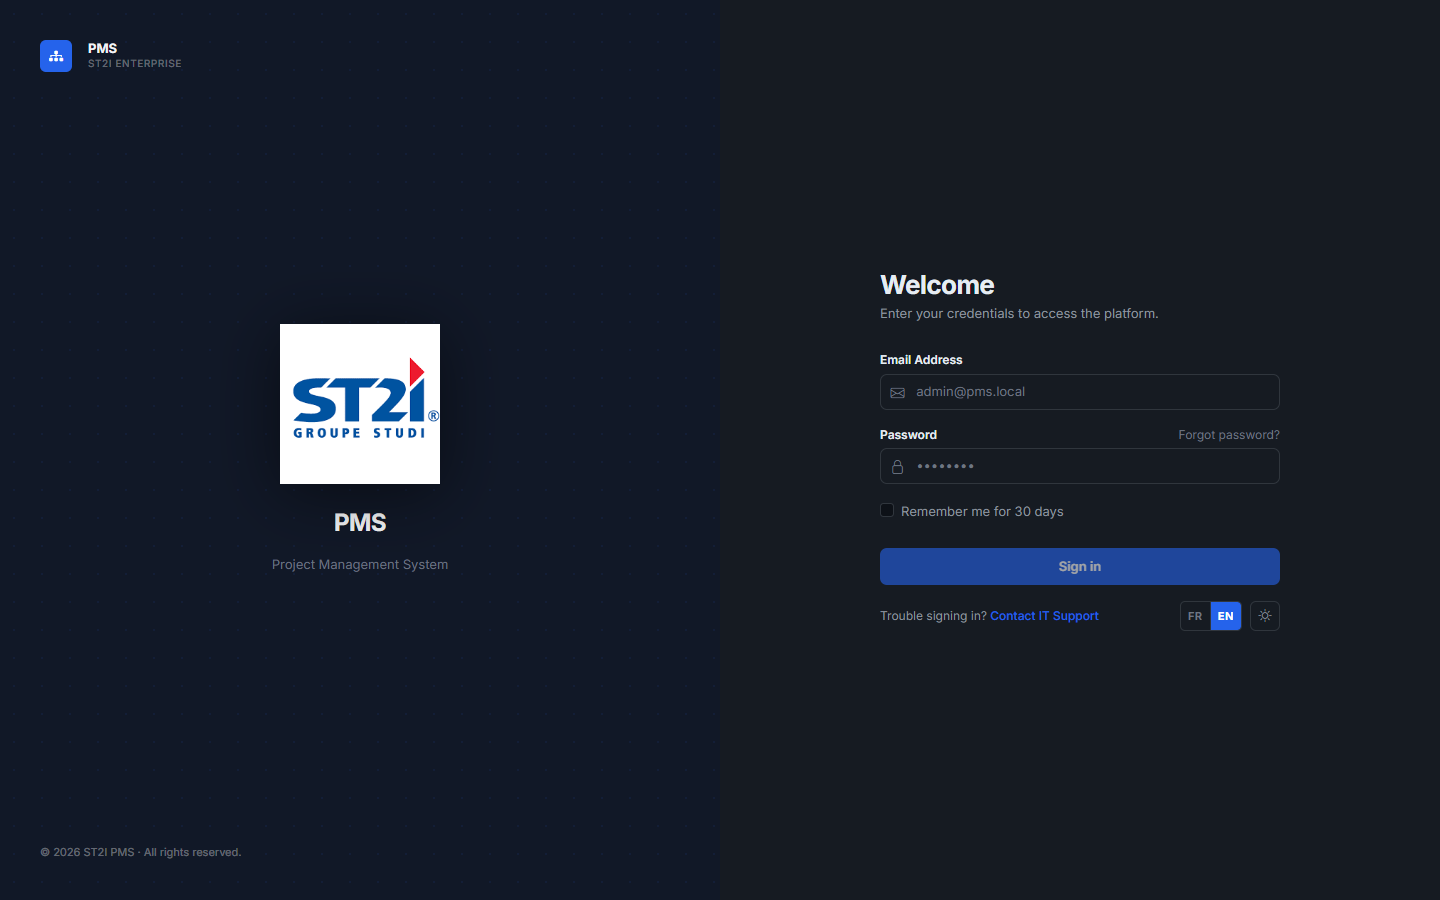
\includegraphics[width=0.8\columnwidth]{img/ui_login.png}
  \caption{Login interface}
  \label{fig:ui-login}
\end{figure}

\emph{\small Note on the screenshots. Every screen reproduced in this chapter and the following
ones was captured against a demonstration dataset generated for the purpose. The project codes,
client names, staff names and amounts they show are fictitious and correspond to no real engagement
of the host organization. No production data appears in this document.}

\begin{figure}[H]
  \centering
  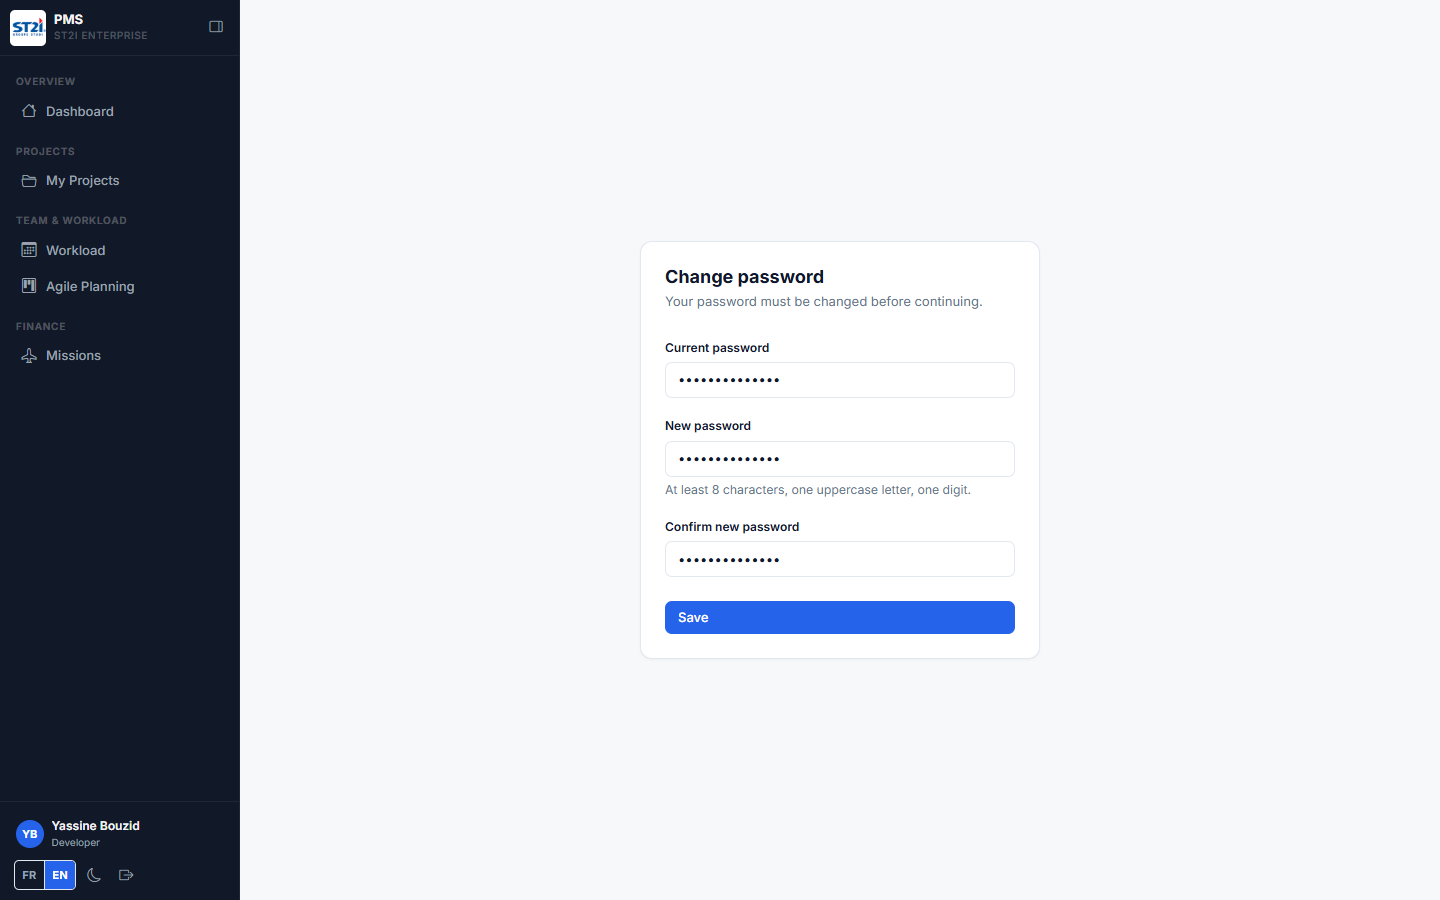
\includegraphics[width=0.8\columnwidth]{img/ui_change_password.png}
  \caption{Forced password change interface}
  \label{fig:ui-change-password}
\end{figure}

% =====================================================================
\section{Sprint 2 --- Dynamic access control, users and resources}

\subsection{Sprint 2 use case diagram}
The sprint covers the administration use cases: assigning permissions to a role, managing user
accounts, and recording resources with their yearly cost rate. All of them are reserved to the
administrator, and all of them include the authentication delivered by sprint~1.

\begin{figure}[H]
  \centering
  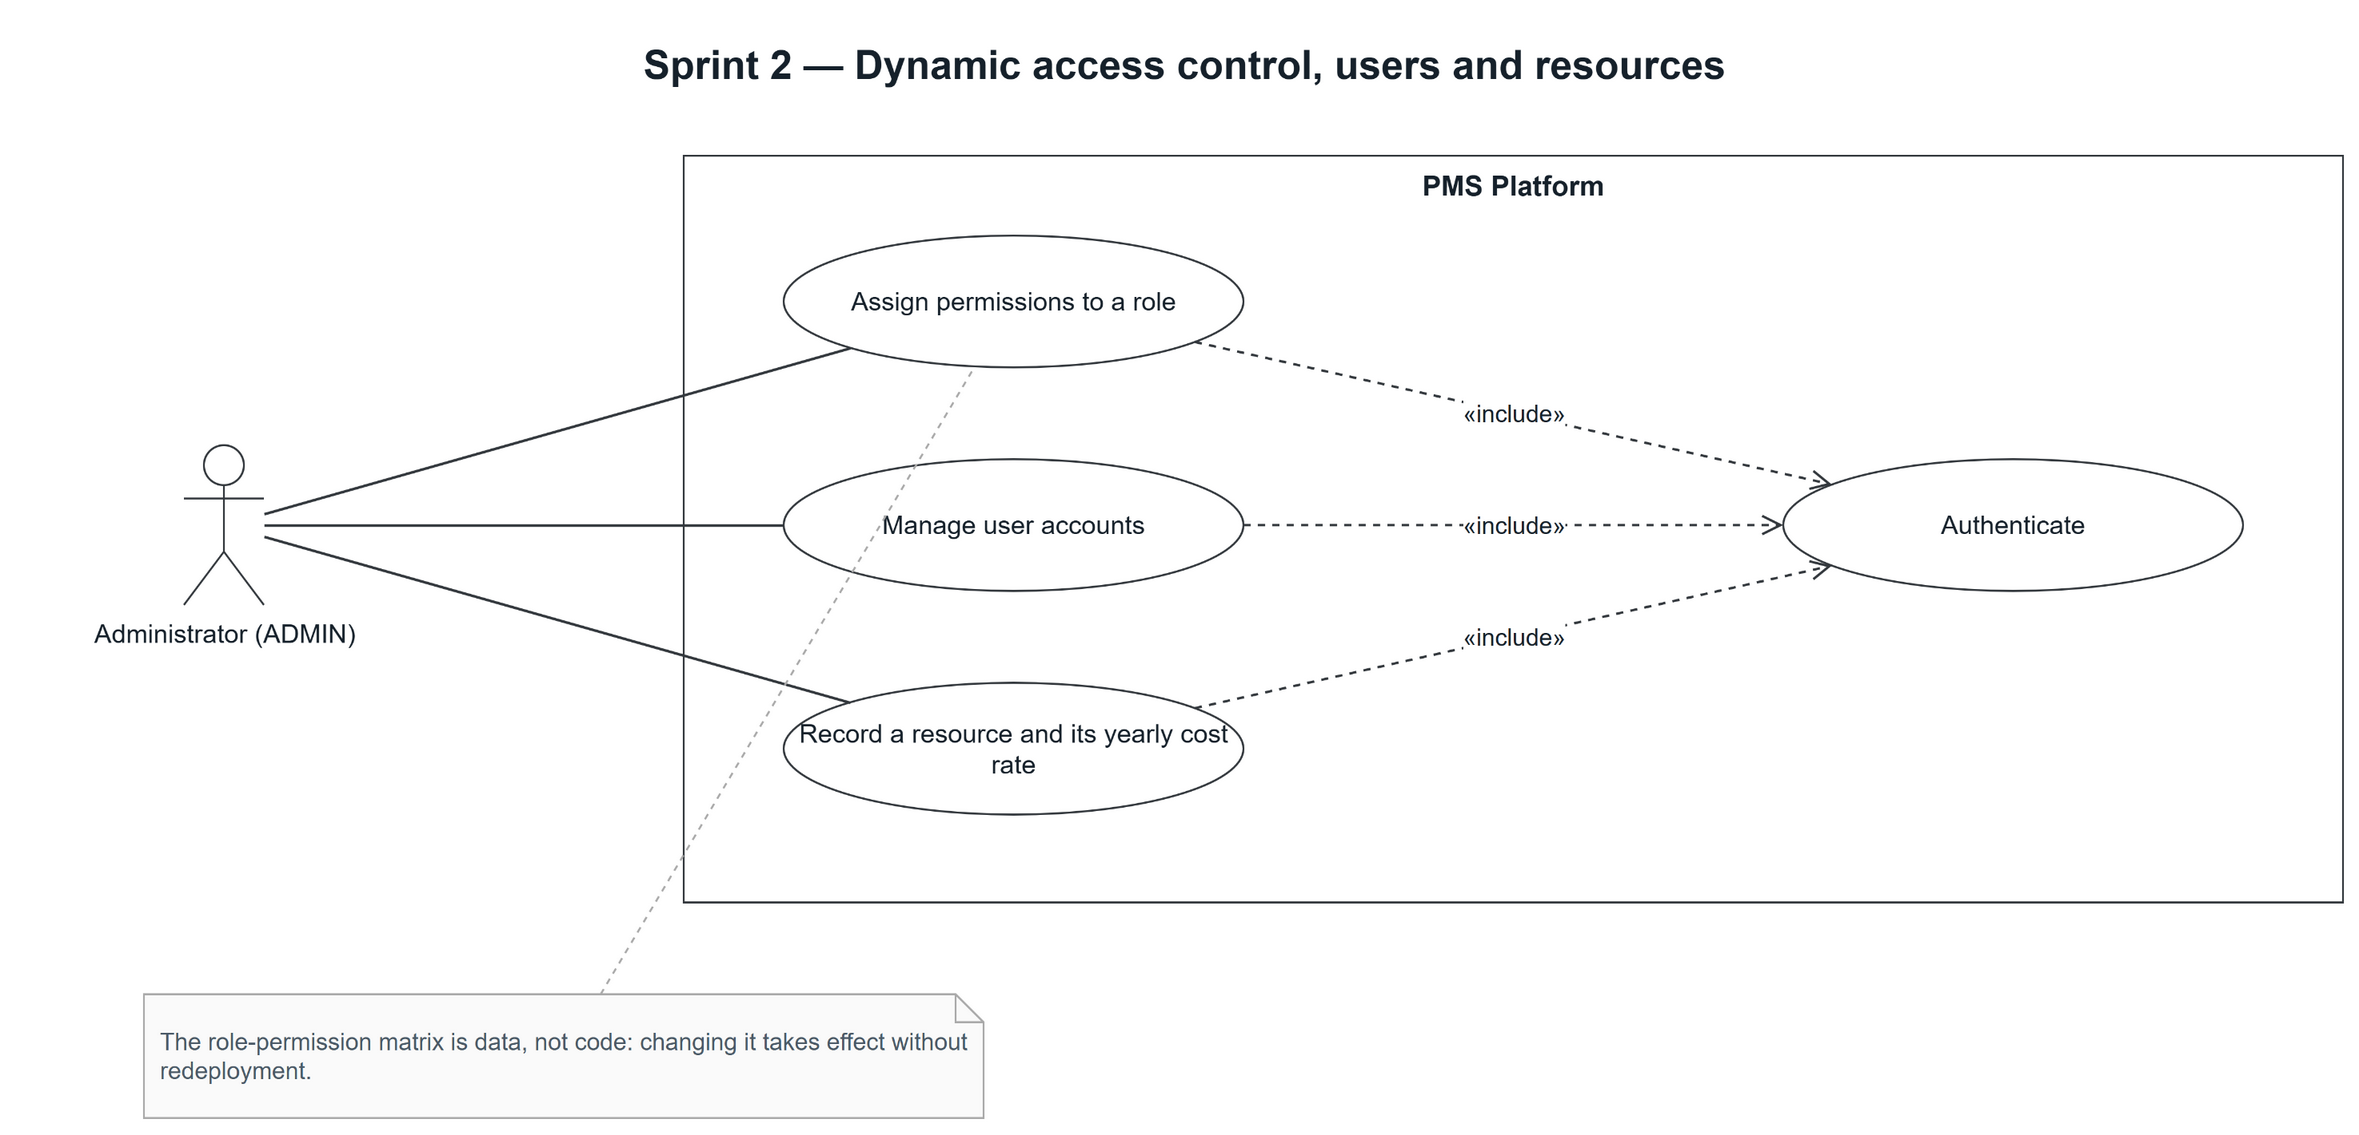
\includegraphics[width=0.75\columnwidth]{img/uc_sprint2.png}
  \caption{Use case diagram of sprint 2}
  \label{fig:uc-s2}
\end{figure}

\subsection{Sprint 2 analysis and design}

\subsubsection{Model of the authorization policy}
The authorization model is the structuring design of the platform and deserves its own class
diagram. A role aggregates permissions, a permission belongs to a functional module, and a user
holds one active role. Nothing in this model is compiled into the application: the association
between a role and its permissions is a table, so the policy is data.

\begin{figure}[H]
  \centering
  
\includegraphics[width=0.85\columnwidth]{img/class_rbac.png}
  \caption{Class diagram of the authorization model}
  \label{fig:class-rbac}
\end{figure}

\subsubsection{Sequence of the ``Grant a permission to a role'' use case}
This scenario is the proof that the policy is configurable. It shows the administrator adding a
permission to a role, the association being persisted, and the affected users obtaining the new
right on their next token without any redeployment.

\begin{figure}[H]
  \centering
  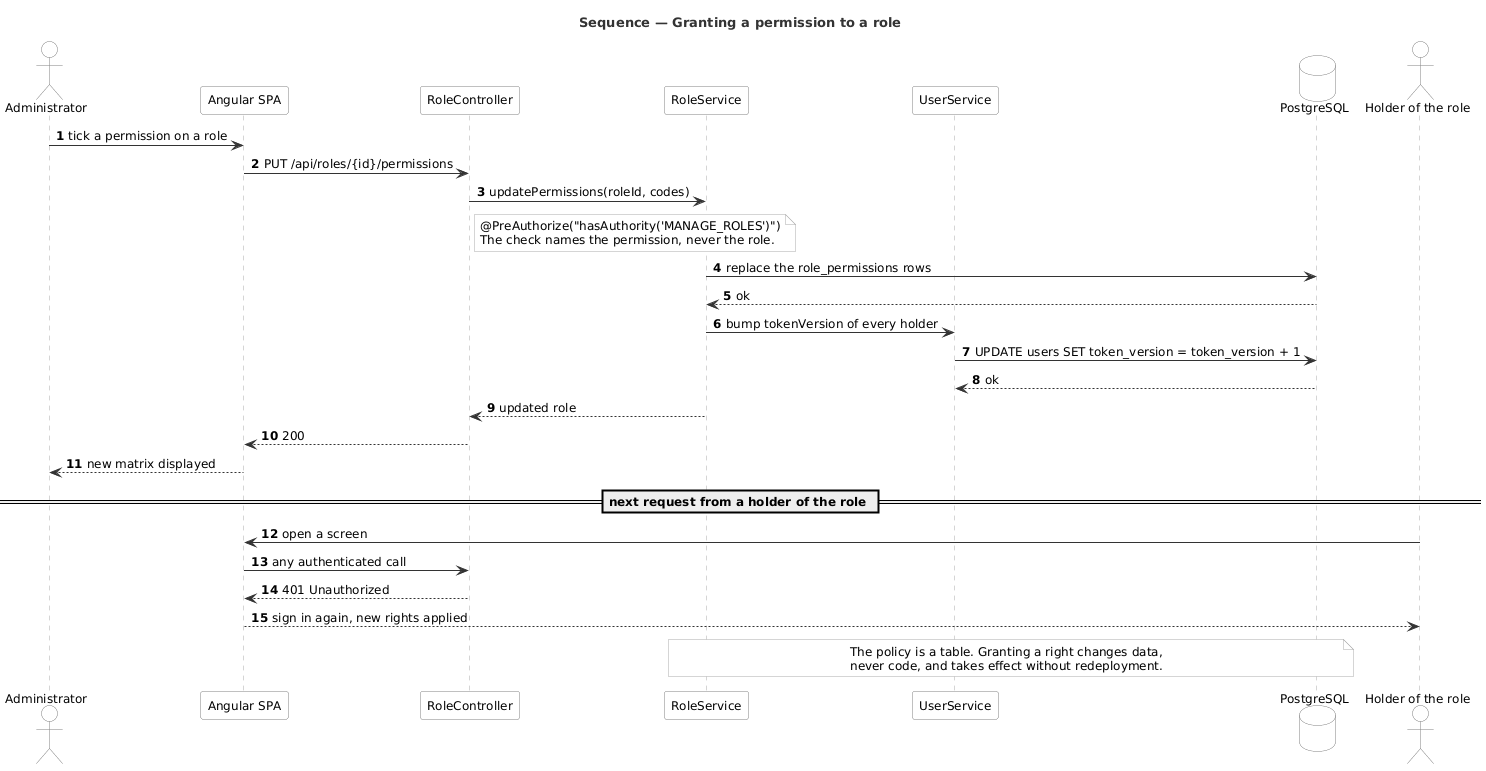
\includegraphics[width=0.95\columnwidth]{img/seq_s2_grant_permission.png}
  \caption{Sequence diagram of the ``Grant a permission to a role'' use case}
  \label{fig:seq-s2-grant}
\end{figure}

\subsubsection{Design decisions}
\textbf{Permissions rather than roles in the code.} No role name is ever tested in the application.
Only permission codes are, through annotations of the form
\texttt{@PreAuthorize("hasAuthority('CREATE\_PROJECT')")}. Testing a role would hard-code the policy
into the source and make every change a release; testing a permission leaves the policy in the
database.

\textbf{A resource is not an account.} A resource represents a cost-bearing capacity and may exist
without a platform account, since the workbook records people who never connect to any system.
Merging the two notions would have made it impossible to cost a contributor who has no login.

\textbf{A cost rate per year, not per resource.} The loaded cost rate is recorded per resource
\emph{and per year}, so that the cost of a man-day uses the rate of the year in which the effort was
booked. This requirement comes directly from the workbook, where the 2024 and 2025 rates of the same
person differ.

\subsection{Sprint 2 realization}

\subsubsection{Permission, role and user model}
The \texttt{role\_permissions} table associates a set of permissions with a role. A user holds a
single active role, but that role can be reconfigured at any time by the administrator without
redeployment. A dedicated migration initialises the four default roles, Administrator, Director,
Project Manager and Developer, with eighteen permission codes spread over seven functional modules.

\subsubsection{Propagation to Spring Security}
The \texttt{JwtAuthenticationFilter} reads the permission codes from the token and converts them
into \texttt{SimpleGrantedAuthority} objects, after which every REST entry point is protected by its
\texttt{@PreAuthorize} annotation.

\subsubsection{Dynamic menu}
The context endpoint returns, for the authenticated user, the list of their permissions together
with their profile information. The Angular frontend builds the navigation menu from that response:
an item is displayed only if the user holds the required permission code. The interface therefore
reflects the authorization policy automatically, with no duplicated rule on the client side.

Figures~\ref{fig:ui-perm-catalogue} to~\ref{fig:ui-dev-dashboard} show the effect on the same
build of the application, signed in as three different roles. The permission catalogue states the
policy; the two dashboards show what it produces.

\begin{figure}[H]
  \centering
  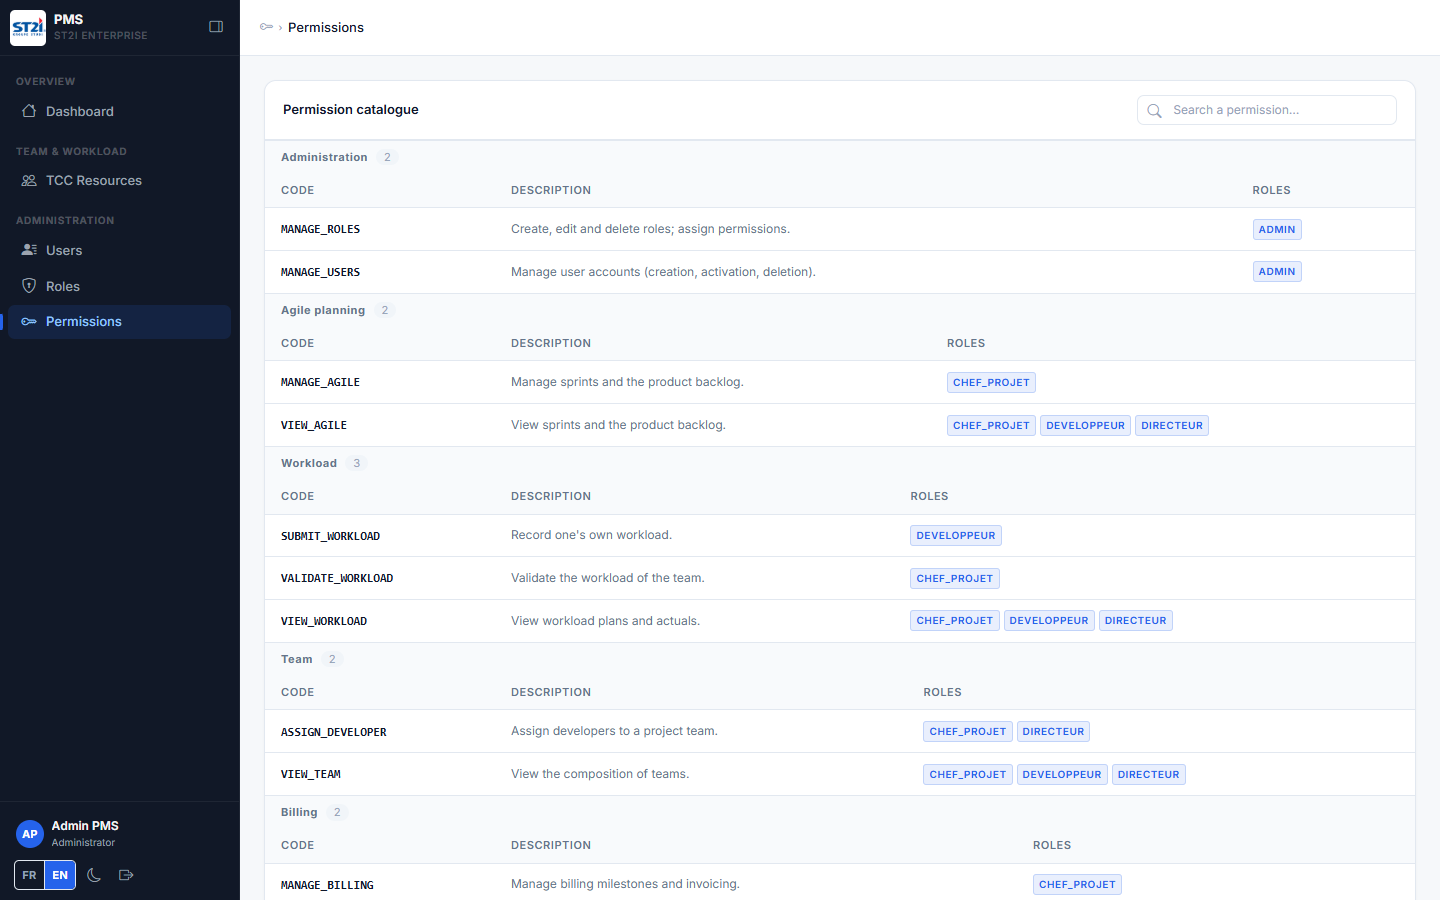
\includegraphics[width=0.92\columnwidth]{img/ui_permissions.png}
  \caption{Permission catalogue: the policy as the administrator reads it, grouped by functional
           module, with the roles that hold each code}
  \label{fig:ui-perm-catalogue}
\end{figure}

\begin{figure}[H]
  \centering
  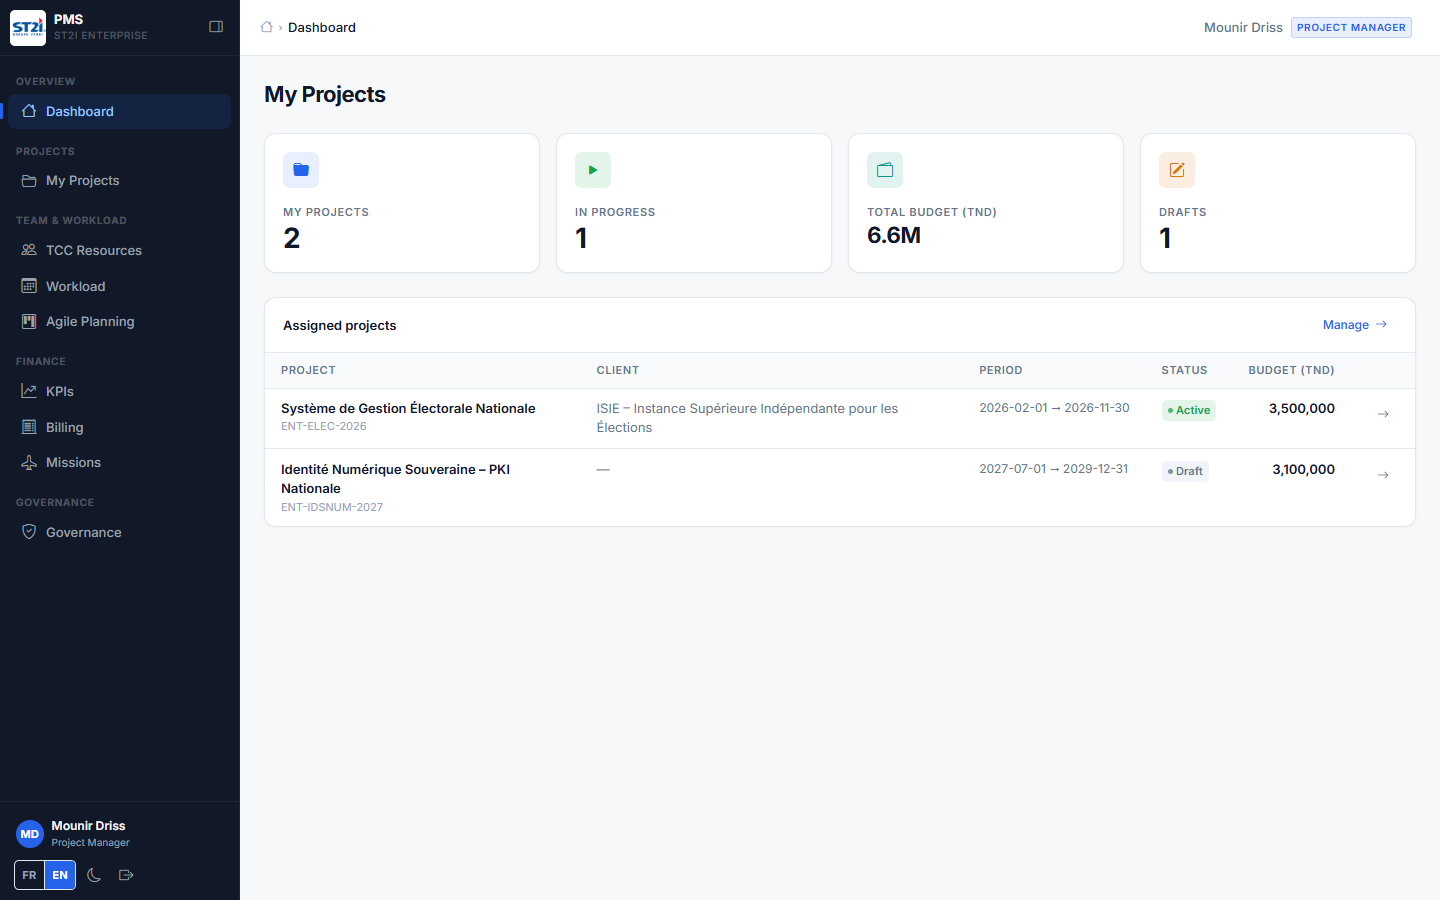
\includegraphics[width=0.92\columnwidth]{img/ui_pm_dashboard.png}
  \caption{Project manager view: the menu carries the finance and governance sections, and the
           workspace is limited to the projects the user manages}
  \label{fig:ui-pm-dashboard}
\end{figure}

\begin{figure}[H]
  \centering
  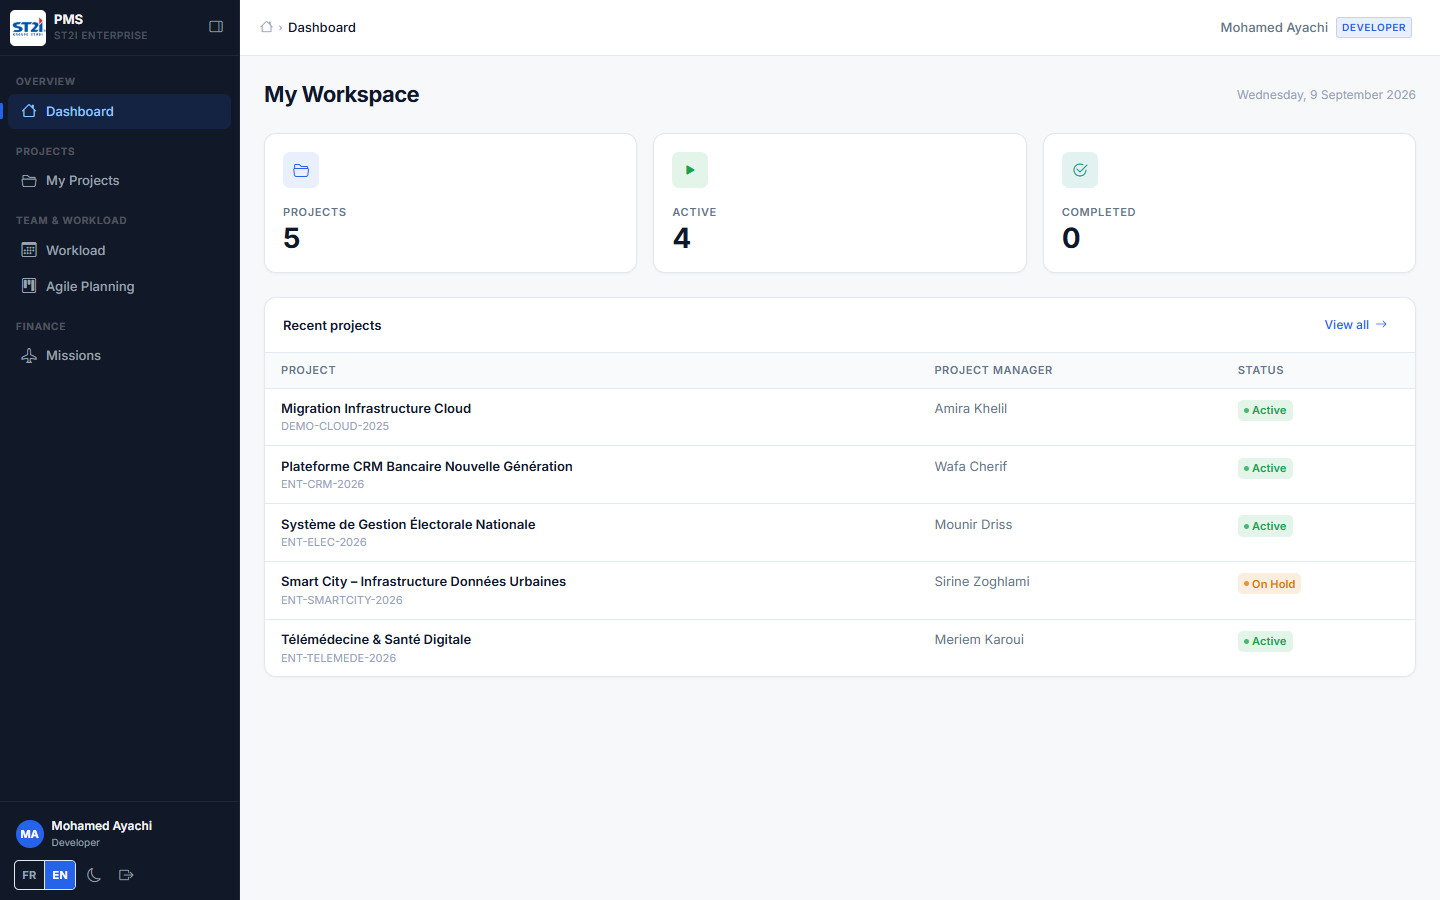
\includegraphics[width=0.92\columnwidth]{img/ui_dev_dashboard.png}
  \caption{Developer view of the same application: no cost rates, no indicators, no billing and no
           governance, because the role holds none of those permission codes}
  \label{fig:ui-dev-dashboard}
\end{figure}

The comparison is the point of the sprint. Nothing distinguishes these two sessions except the
row that links their account to a role, and the rows that link that role to permissions. No branch
in the code names a role, and no menu is hidden by a hard-coded condition: removing
\texttt{VIEW\_KPI} from the developer role removes the entry, and granting it back restores it, in
both cases without recompiling anything. The requirement that a developer must never see the margin
of the project they work on is met by the absence of a row, not by an \texttt{if}.

\subsubsection{Users and resources}
The \texttt{user} module manages accounts, that is creation by the administrator with a temporary
password, modification, activation and deactivation, and role assignment, together with the human
resources and their daily and loaded cost rates. Conversions between entities and data transfer
objects are handled by MapStruct mappers.

\begin{figure}[H]
  \centering
  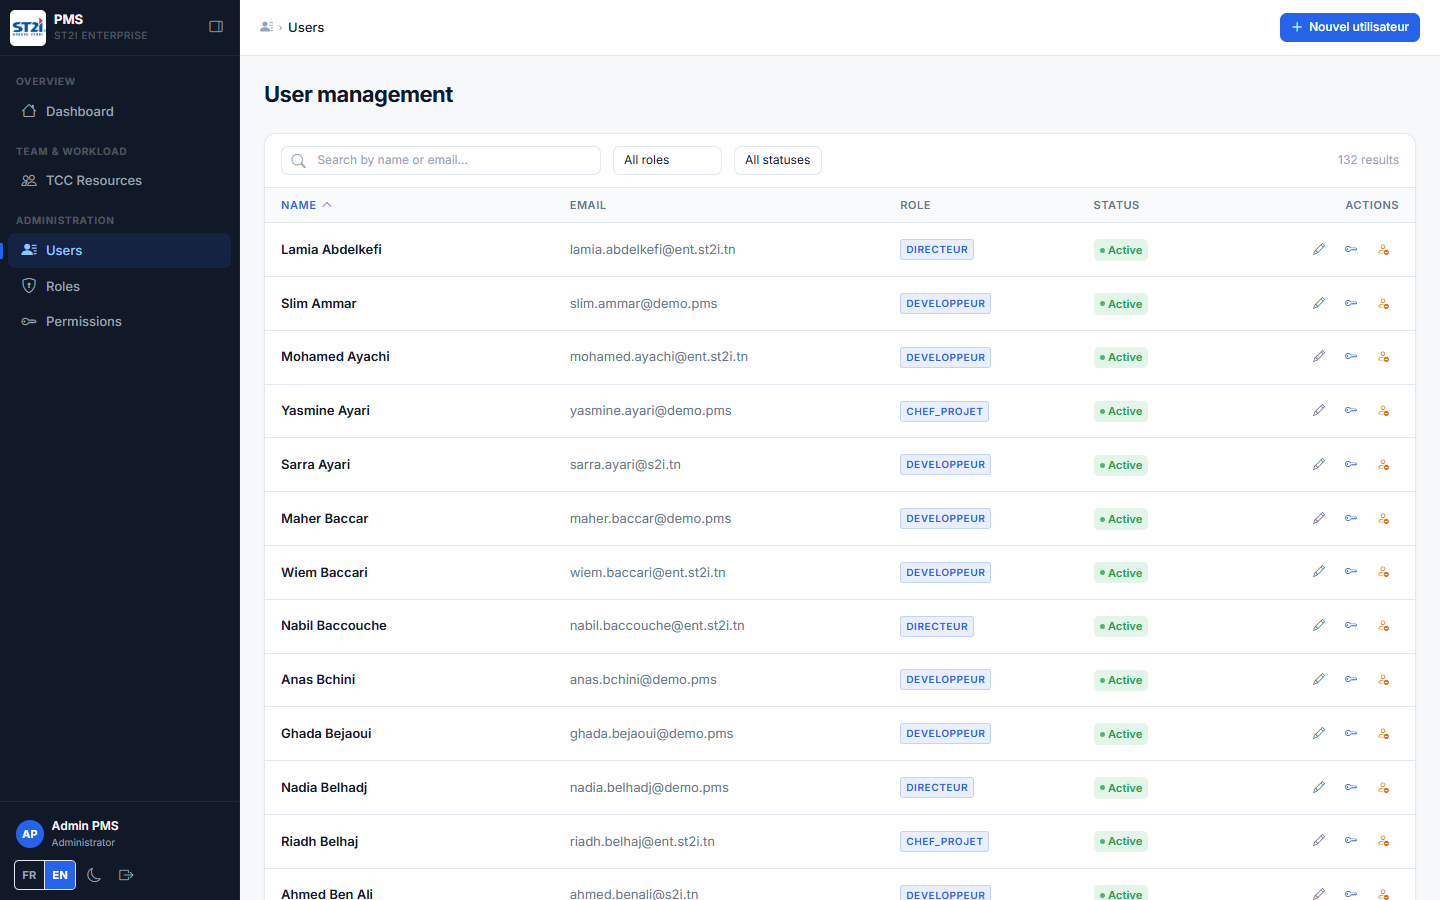
\includegraphics[width=0.9\columnwidth]{img/ui_users.png}
  \caption{User management interface}
  \label{fig:ui-users}
\end{figure}

\begin{figure}[H]
  \centering
  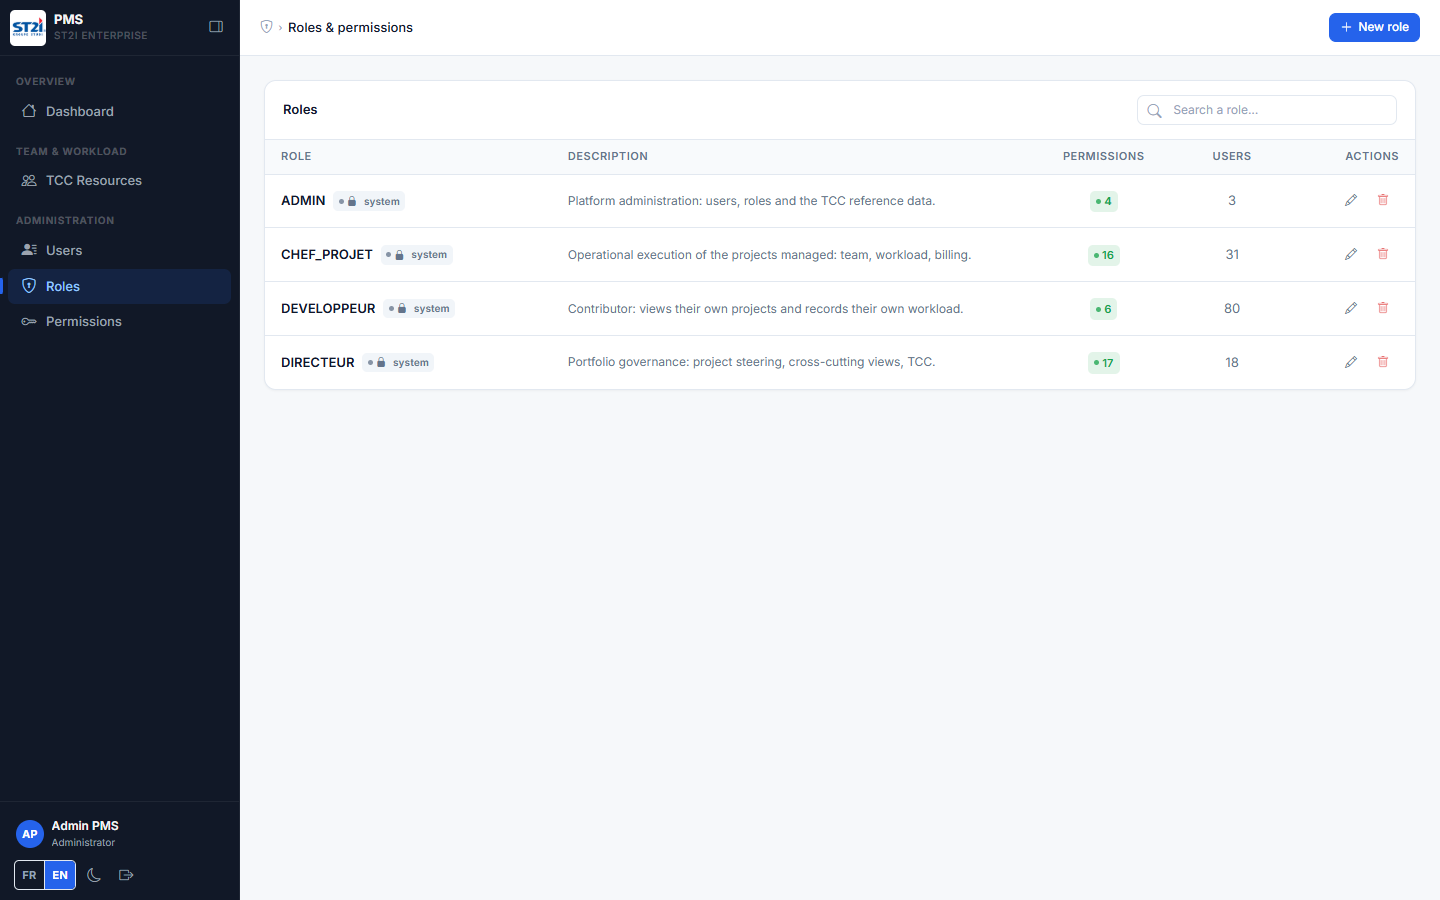
\includegraphics[width=0.9\columnwidth]{img/ui_roles.png}
  \caption{Role and permission management interface}
  \label{fig:ui-roles}
\end{figure}

\begin{figure}[H]
  \centering
  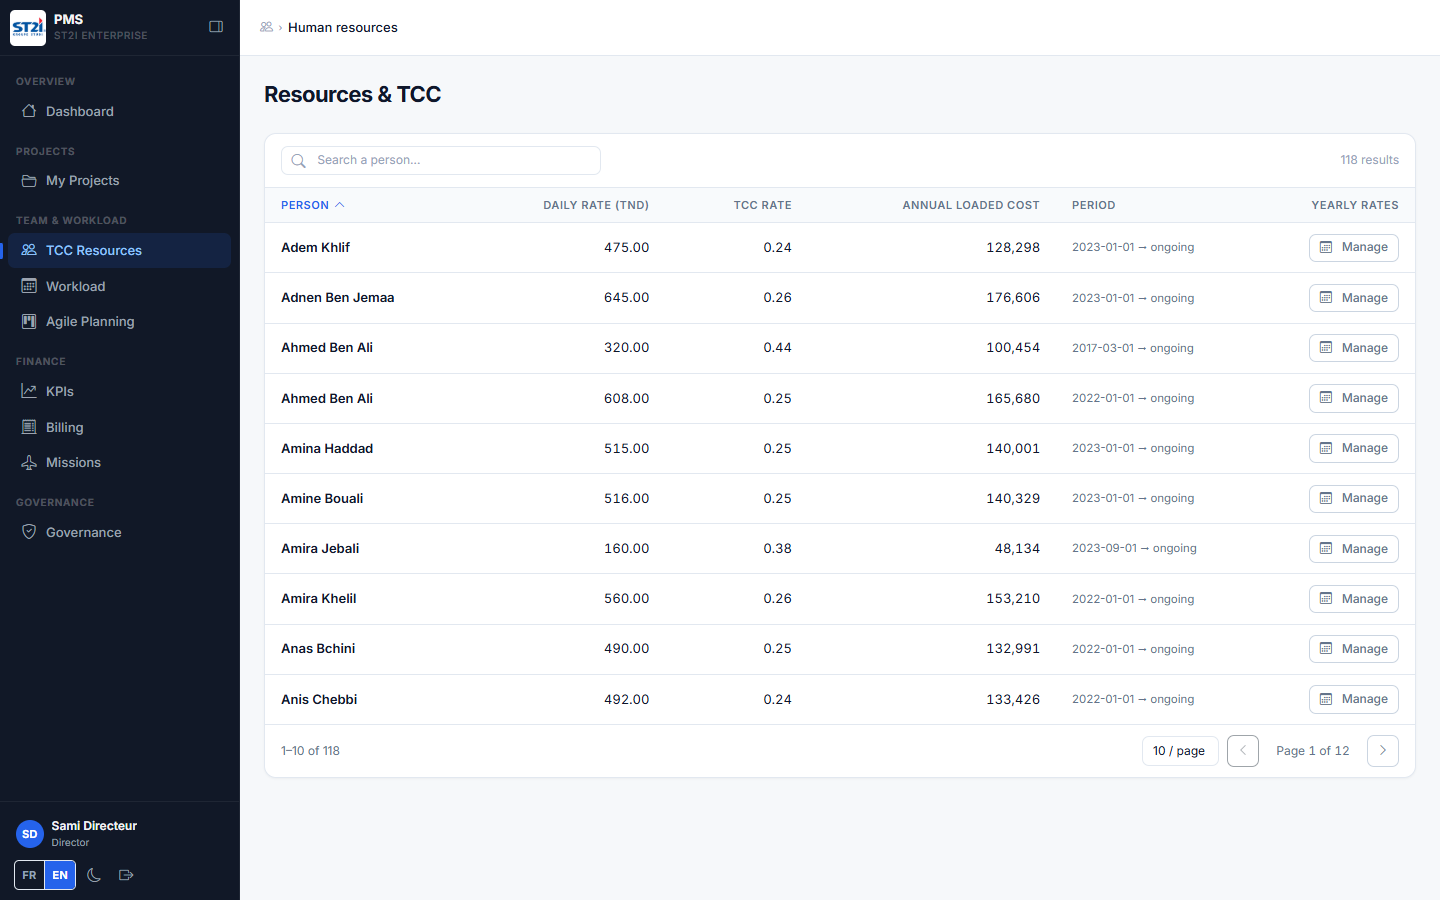
\includegraphics[width=0.9\columnwidth]{img/ui_resources.png}
  \caption{Resource and yearly cost rate interface}
  \label{fig:ui-resources}
\end{figure}

\section*{Conclusion}
Release~1 established the foundations on which the entire platform rests: a modular application
skeleton with auditing and controlled migrations, a robust authentication chain, and above all a
dynamic authorization model that makes the security policy configurable data rather than compiled
code. The platform now knows not only who the user is but what that user may do, and it holds the
reference data the business modules consume. The next release exploits this foundation to deliver
the operational management of projects and workload.

        \clearpage

        \chapter{Release 2 --- Project and Operational Management}

\section*{Introduction}
Release~1 delivered a secured and administrable platform, but one that managed no project. This
release opens operational steering. Sprint~3 introduces the central entity of the whole domain ---
the project, with its controlled lifecycle and its budget; Sprint~4 populates it with a team and
with the workload data on which every later indicator depends.

At the end of this release, a project can be created, staffed, planned, and its actual consumption
recorded: everything the financial engine of Release~3 will need as input.

% =====================================================================
\section{Sprint 3 --- Project Management and Lifecycle}

\subsection{Sprint Objective}
Deliver the management of projects: creation with their contractual and financial identity,
assignment of a project manager, and a lifecycle that the application enforces rather than merely
documents.

\subsection{Functional Scope}
This sprint covers user stories US-08 to US-10: creating and configuring a project, controlling its
status transitions, and assigning its project manager.

\subsection{Features Implemented}
\begin{itemize}
  \item Project creation with code, client, funder, engagement type, currency and budget.
  \item Controlled status lifecycle with server-side enforcement.
  \item Effective budget derived from the initial budget and its amendments.
  \item Project manager assignment, with a single active assignment at a time.
  \item Project archiving, distinct from closure.
\end{itemize}

\subsection{Technical Realisation}

\subsubsection{Project identity}
The \texttt{project} module reproduces the identification sheet of the reference workbook: project
code, client, funder, business model, engagement type (fixed price or time~\&~material), project
currency with its contractual exchange rate, initial budget, sold workload and provisions. The
class model of the module is given in Figure~\ref{fig:class-proj}.

\begin{figure}[H]
  \centering
  
\includegraphics[width=0.85\columnwidth]{img/class_project_team.png}
  \caption{Class diagram --- projects and teams}
  \label{fig:class-proj}
\end{figure}

\subsubsection{A lifecycle enforced by the domain}
A project moves through five states: \texttt{DRAFT}, \texttt{ACTIVE}, \texttt{ON\_HOLD},
\texttt{COMPLETED} and \texttt{CANCELLED}. Not every transition is legal: a completed project
cannot return to draft, a cancelled project is terminal.

The rule is carried by the enumeration itself, through a \texttt{canTransitionTo} operation that
each status answers for its own legal successors. The service layer consults it before any status
change and rejects an illegal transition with \texttt{HTTP 422 Unprocessable Entity}. Placing the
rule in the domain rather than in the controller guarantees that no future entry point can bypass
it.

\begin{figure}[H]
  \centering
  
\includegraphics[width=0.7\columnwidth]{img/state_project.png}
  \caption{State diagram --- project lifecycle}
  \label{fig:state}
\end{figure}

Archiving is deliberately \textbf{not} a state but a flag on a completed project: an archived
project leaves the active lists while remaining restorable, which a terminal state would not allow.

\subsubsection{Effective budget}
A project carries an initial budget and, once amendments exist, a revised budget. Every computation
uses the \textbf{effective budget}: the revised budget when it is defined, the initial budget
otherwise. This value has a \textbf{single writer}, the amendment, which prevents the two
figures from drifting apart, a failure mode observed in the original workbook where the budget was
edited in several places.

\subsubsection{Project manager assignment}
A project has exactly one active project manager at any time, but keeps the history of previous
assignments. Assigning a new manager therefore closes the current assignment rather than
overwriting it, preserving the traceability required for auditing.

% TODO: capture as img/ui_projects.png and img/ui_project_detail.png, then uncomment.
% \begin{figure}[H]
%   \centering
%   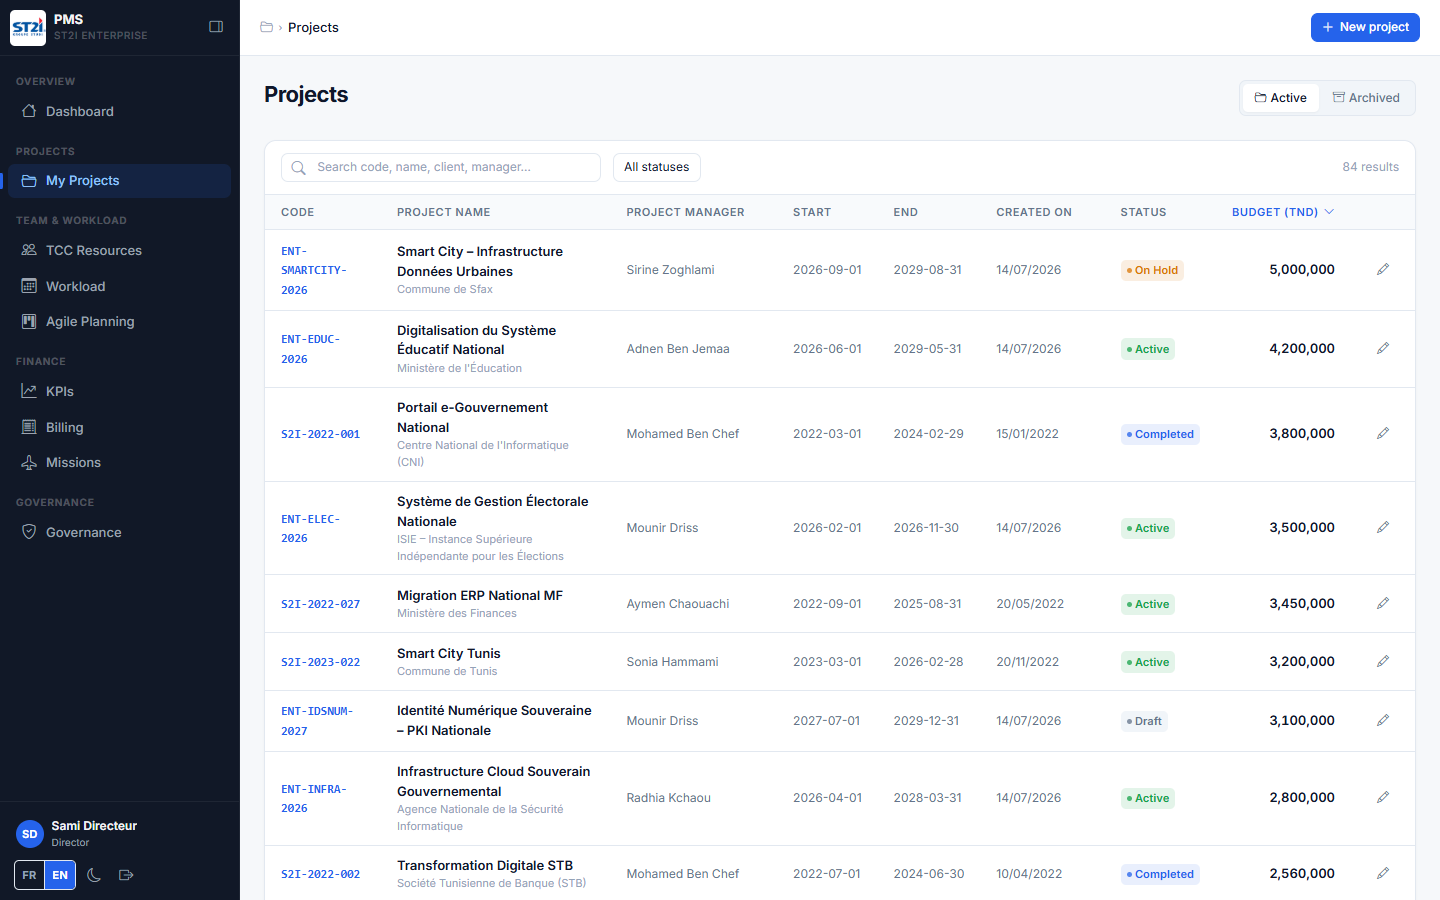
\includegraphics[width=0.95\columnwidth]{img/ui_projects.png}
%   \caption{Project list interface}
%   \label{fig:ui-projects}
% \end{figure}

\subsection{Tests and Validation}
Validation focuses on the lifecycle, since it is the rule most likely to be violated by a client
application.

\begin{longtable}{|m{4.2cm}|m{5.4cm}|m{4.8cm}|}
\hline
\textbf{Test case} & \textbf{Steps} & \textbf{Expected result} \\
\hline
\endhead
\endfoot
\endlastfoot
\hline
Legal transition & Move a project from \texttt{DRAFT} to \texttt{ACTIVE} & HTTP 200, status updated
\\
\hline
Illegal transition & Move a project from \texttt{COMPLETED} back to \texttt{DRAFT} & HTTP 422,
status unchanged \\
\hline
Terminal state & Attempt any transition out of \texttt{CANCELLED} & HTTP 422 \\
\hline
Effective budget & Add an amendment then read the project & Computations use the revised budget \\
\hline
Manager assignment & Assign a second project manager & Previous assignment closed, one active
manager remains \\
\hline
\caption{Test cases --- Sprint 3}
\label{tab:tests-s3}
\end{longtable}

\subsection{Sprint Outcome}
Projects exist, carry their contractual and financial identity, and follow a lifecycle the
application enforces. The invalid states that a spreadsheet cannot prevent are now structurally
impossible.

\subsection{Transition to the Next Sprint}
A project without a team consumes nothing and produces no indicator. Sprint~4 therefore staffs the
project and captures the effort planned and consumed, the raw material of the whole financial
model.

% =====================================================================
\section{Sprint 4 --- Teams and Workload Management}

\subsection{Sprint Objective}
Allow a project manager to build the project team, plan the monthly workload, and let developers
record the effort actually consumed, with the guarantees of integrity the indicators will depend
on.

\subsection{Functional Scope}
This sprint covers user stories US-11 to US-14: building the team, planning the workload,
submitting actual workload, and validating it.

\subsection{Features Implemented}
\begin{itemize}
  \item Assignment and removal of team members, with preserved history.
  \item Monthly workload planning per resource.
  \item Submission of actual workload, restricted to assigned projects.
  \item Validation of submitted workload by the project manager.
  \item Immutability of a validated period.
\end{itemize}

\subsection{Technical Realisation}

\subsubsection{Team assignment}
A team assignment links a user to a project with a role in the team and a validity period. A
developer may belong to several projects simultaneously. Removing a member closes the assignment
rather than deleting it, so that past workload remains attributable.

Assignment is protected by \textbf{two distinct checks}, illustrated in
Figure~\ref{fig:seq-assign}: the caller must hold the \texttt{ASSIGN\_DEVELOPER} permission
\emph{and} the target project must fall within their scope. The permission answers ``what may I
do''; the scope answers ``on which projects''. Conflating the two would let a project manager act
on a project that is not theirs.

\begin{figure}[H]
  \centering
  
\includegraphics[width=0.95\columnwidth]{img/seq_assign_developer.png}
  \caption{Sequence --- assigning a developer, permission and scope}
  \label{fig:seq-assign}
\end{figure}

\subsubsection{Two kinds of workload}
The model distinguishes the \textbf{workload plan} (what is forecast) from the \textbf{actual
workload} (what was consumed). Both are stored as a monthly time series, one row per project,
resource and month, rather than as a wide grid of month columns.

\subsubsection{Period normalisation and uniqueness}
A month is stored as the first day of that month. This normalisation is what makes uniqueness
enforceable: without it, two entries for the same month recorded on different days would coexist
silently. A unique partial index guarantees a single retained value per cell, and it is that value
which feeds the indicator engine.

\subsubsection{Validation and immutability}
A developer submits their own workload, on assigned projects only. The project manager then
validates it. Once a period is validated it becomes \textbf{immutable}: a later correction cannot
silently rewrite a month on which a monthly review has already been based. This constraint is the
direct answer to the traceability weakness identified in the Excel process.

% TODO: capture as img/ui_workload.png, then uncomment.
% \begin{figure}[H]
%   \centering
%   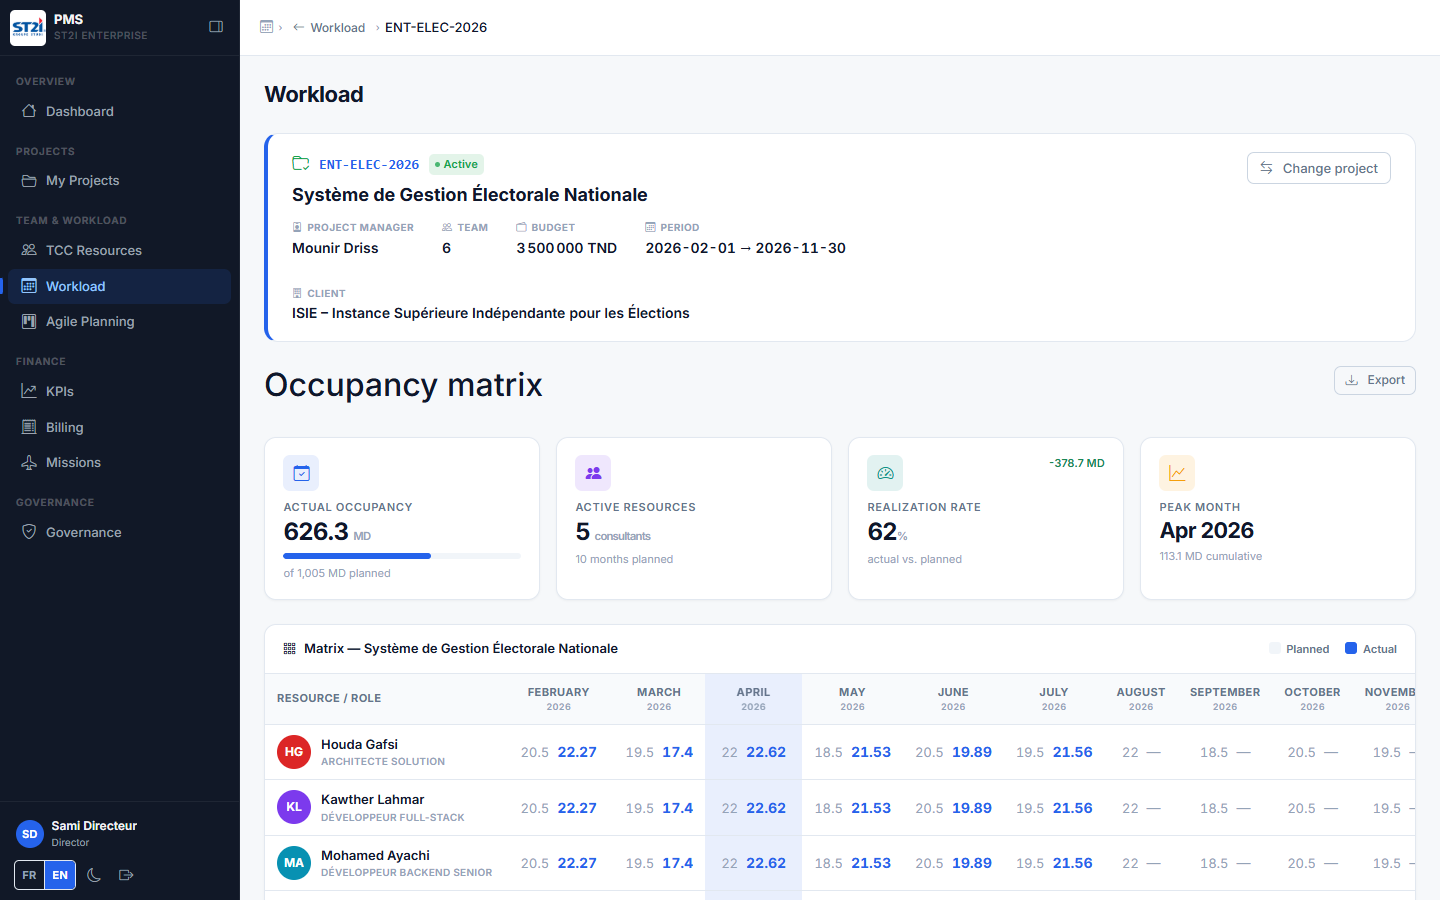
\includegraphics[width=0.95\columnwidth]{img/ui_workload.png}
%   \caption{Workload matrix interface}
%   \label{fig:ui-workload}
% \end{figure}

\subsection{Tests and Validation}

\begin{longtable}{|m{4.2cm}|m{5.4cm}|m{4.8cm}|}
\hline
\textbf{Test case} & \textbf{Steps} & \textbf{Expected result} \\
\hline
\endhead
\endfoot
\endlastfoot
\hline
Authorised assignment & Assign a developer with the permission, on a project in scope & HTTP 201,
assignment recorded \\
\hline
Out-of-scope assignment & Assign on a project outside the caller's scope & HTTP 403 \\
\hline
Submission on an unassigned project & Submit workload on a project the developer is not assigned to
& Refused \\
\hline
Duplicate month & Submit twice for the same project, resource and month & A single retained value
\\
\hline
Validated period & Modify a period already validated & Refused, period immutable \\
\hline
\caption{Test cases --- Sprint 4}
\label{tab:tests-s4}
\end{longtable}

\subsection{Sprint Outcome}
Projects now carry a team, a forecast and a measured consumption, all captured under integrity
constraints that a spreadsheet cannot express: no duplicate month, no entry on an unassigned
project, no silent rewriting of a validated period.

\subsection{Transition to the Next Sprint}
The cost side of the project is now measurable. The revenue side is not: nothing yet records what
is invoiced, nor the expenses that weigh on the margin. Release~3 delivers the financial and
governance value of the platform, starting with billing and missions.

\section*{Conclusion}
Release~2 turned a secured shell into an operational tool: projects with an enforced lifecycle,
teams with traceable assignments, and workload captured as a reliable monthly time series. The data
required by the financial engine is now available and trustworthy, which is the precondition for
the indicators built in the next release.

        \clearpage

        \chapter{Release 3: Financial Management and Governance}

\section*{Introduction}
\addcontentsline{toc}{section}{Introduction}
This release delivers what the platform was commissioned for: replacing the financial logic of the
Excel workbook. Sprint~6 records the revenue side, that is billing milestones, payments and
amendments, together with the mission expenses that eat into the margin. Sprint~7 adds the
governance registers, which document the life of a project. Sprint~8 closes the loop with the
internal quote and the indicator engine. That engine reads everything built since Release~1.
\section{Sprint 6 --- Billing and missions}

\subsection{Sprint objectives}
Sprint~6 ran from 25~May to 12~June, three weeks (Table~\ref{tab:schedule}). Its objective is to
open the financial side. Milestones carry the invoicing, payments track what has been collected,
amendments move the budget, and missions bring travel cost into the project.

\subsection{Sprint backlog}
The sprint commits the following items of the product backlog (Table~\ref{tab:backlog}).

\begin{longtable}{|m{1.6cm}|m{12.4cm}|}
\caption{Sprint 6 backlog}\label{tab:sb6}\\
\hline
\textbf{Story} & \textbf{User story} \\
\hline
\endfirsthead
\hline
\textbf{Story} & \textbf{User story} \\
\hline
\endhead
\endfoot
\endlastfoot
\hline
US-20 & As a project manager, I want to define billing milestones following contractual progress \\
\hline
US-21 & As a project manager, I want to record payments received against a milestone \\
\hline
US-22 & As a project manager, I want to record amendments so the revised budget reflects contractual change \\
\hline
US-23 & As a project manager, I want to include travel costs in the project cost \\
\hline
\end{longtable}

\subsection{Task planning}
The author being the sole developer, each item was expanded directly into the technical work it
required rather than distributed across a team.

\begin{longtable}{|m{1.6cm}|m{12.4cm}|}
\caption{Sprint 6 task planning}\label{tab:tp6}\\
\hline
\textbf{Story} & \textbf{Technical work} \\
\hline
\endfirsthead
\hline
\textbf{Story} & \textbf{Technical work} \\
\hline
\endhead
\endfoot
\endlastfoot
\hline
US-20 & Milestone as a percentage of the effective budget, sum capped at 100\% in the service layer \\
\hline
US-21 & Payments kept as individual rows so partial settlements stay visible \\
\hline
US-22 & Amendment as the single writer of the revised budget \\
\hline
US-23 & Mission with typed components, each converted at the mission date before summation \\
\hline
\end{longtable}

\subsection{Design}
The sprint covers the use cases through which a project earns and spends outside labour: defining a
billing milestone, invoicing it, recording a payment against it, recording a contractual amendment,
and recording a mission with its expenses. All are reserved to the project manager, except the
amendment, which the director records because it changes the contract.

\begin{figure}[H]
  \centering
  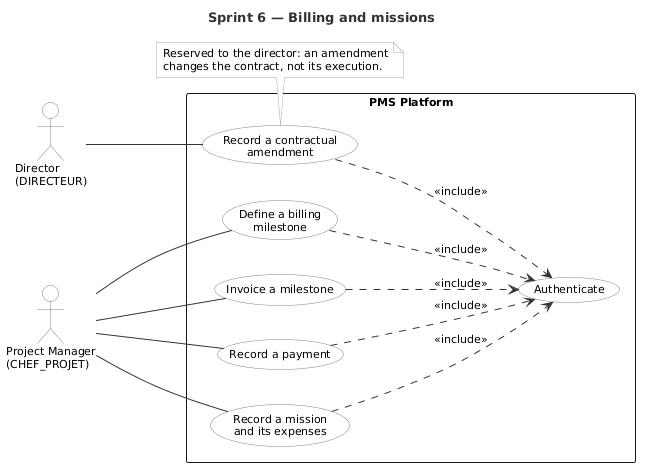
\includegraphics[width=0.75\columnwidth]{img/uc_sprint6.png}
  \caption{Use case diagram of sprint 6}
  \label{fig:uc-s6}
\end{figure}

\runin{Model of billing and missions}
A milestone belongs to one project and carries a label, a percentage of the contract, an amount, a
due date and a status. A mission belongs to a project and an employee, and decomposes into typed
cost components.

\begin{figure}[H]
  \centering
  
\includegraphics[width=0.95\columnwidth]{img/class_financial.png}
  \caption{Class diagram --- financial management}
  \label{fig:class-fin}
\end{figure}

\runin{Design decisions}
\textbf{The milestone amount is derived, not stored.} It follows from the effective budget and the
percentage, so an amendment propagates automatically to every milestone not yet invoiced. Storing
the amount would have required updating each milestone on every amendment, and any missed update
would have gone unnoticed.

\textbf{The sum of percentages may not exceed 100\%.} This rule is inherited from the workbook,
where it was a convention the spreadsheet could not enforce. Here it is checked in the service
layer, and an attempt to exceed it is rejected rather than silently accepted.

\textbf{Payments are rows, not a settled total.} Keeping a single settled amount would lose the
history of partial settlements, which is precisely what a project manager chasing collection needs
to see.

\textbf{Conversion happens before summation, never after.} A mission may be incurred in a currency
different from the reporting one. Each component is converted at the rate of the mission date and
only then summed. Summing first would add amounts expressed in different currencies, and the total
would be meaningless while still looking plausible.

\subsection{Implementation}
The module opens on the milestone, which carries the invoicing, and the amendment, which is the
only thing allowed to move the budget.


\runin{Milestone lifecycle}
A milestone moves through three states: planned, invoiced and paid. Invoicing records the invoice
date; a payment recorded against an invoiced milestone moves it to paid.

\runin{Amendments}
An amendment carries a reference, an amount and an impact on the sold workload. It is the single
writer of the revised budget introduced in Sprint~3, which is what keeps the contractual and
financial history coherent.

\begin{figure}[H]
  \centering
  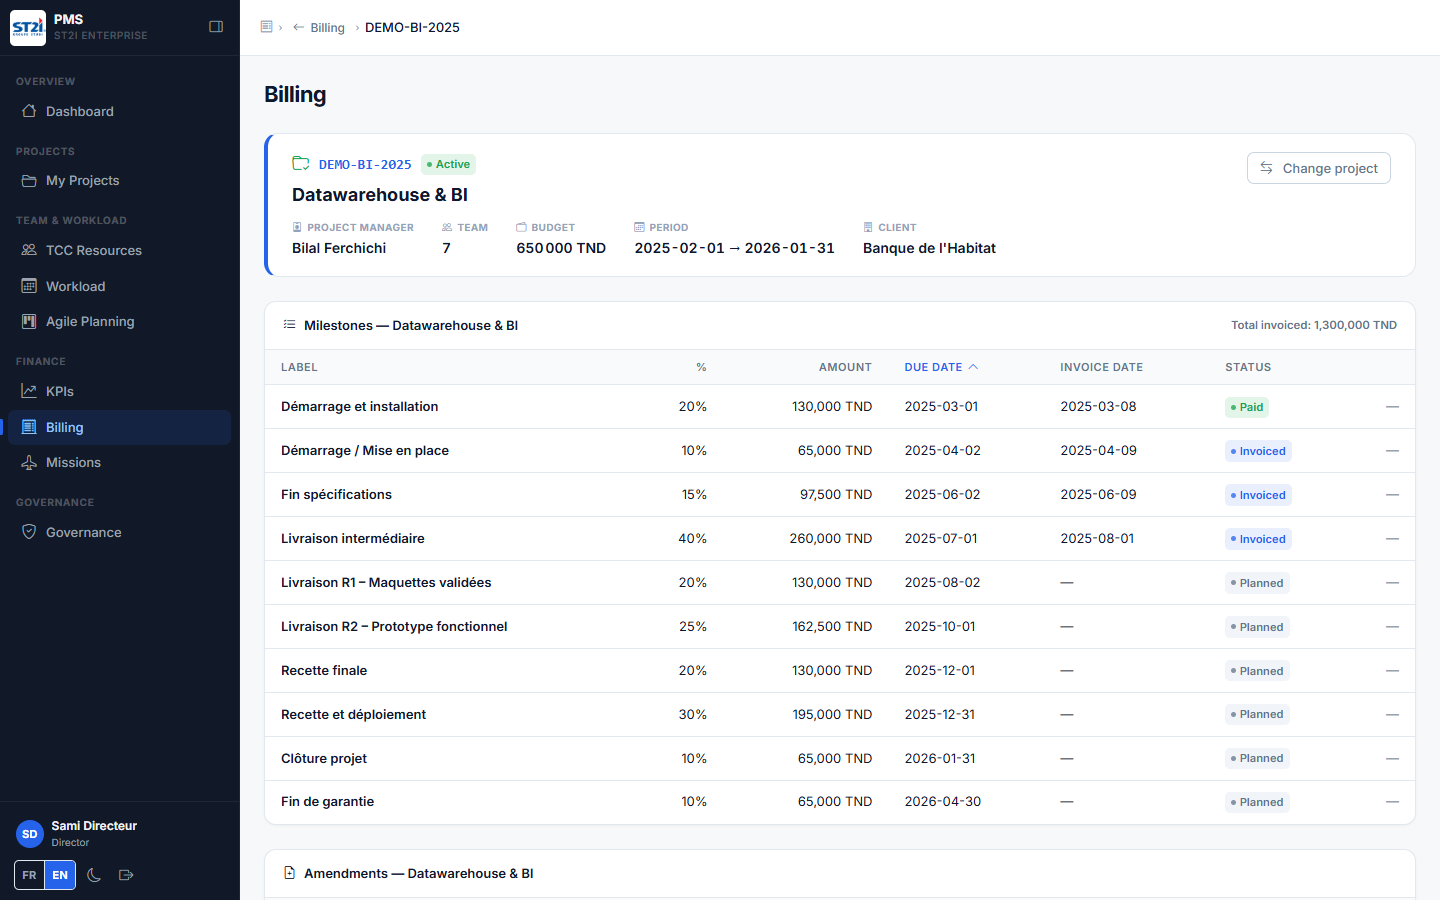
\includegraphics[width=0.95\columnwidth]{img/ui_billing.png}
  \caption{Billing milestones interface}
  \label{fig:ui-billing}
\end{figure}

Missions are recorded on their own screen, each one decomposed into the typed cost components
the workbook already used: per diem, ticket, transport, accommodation and stamp duty.

\begin{figure}[H]
  \centering
  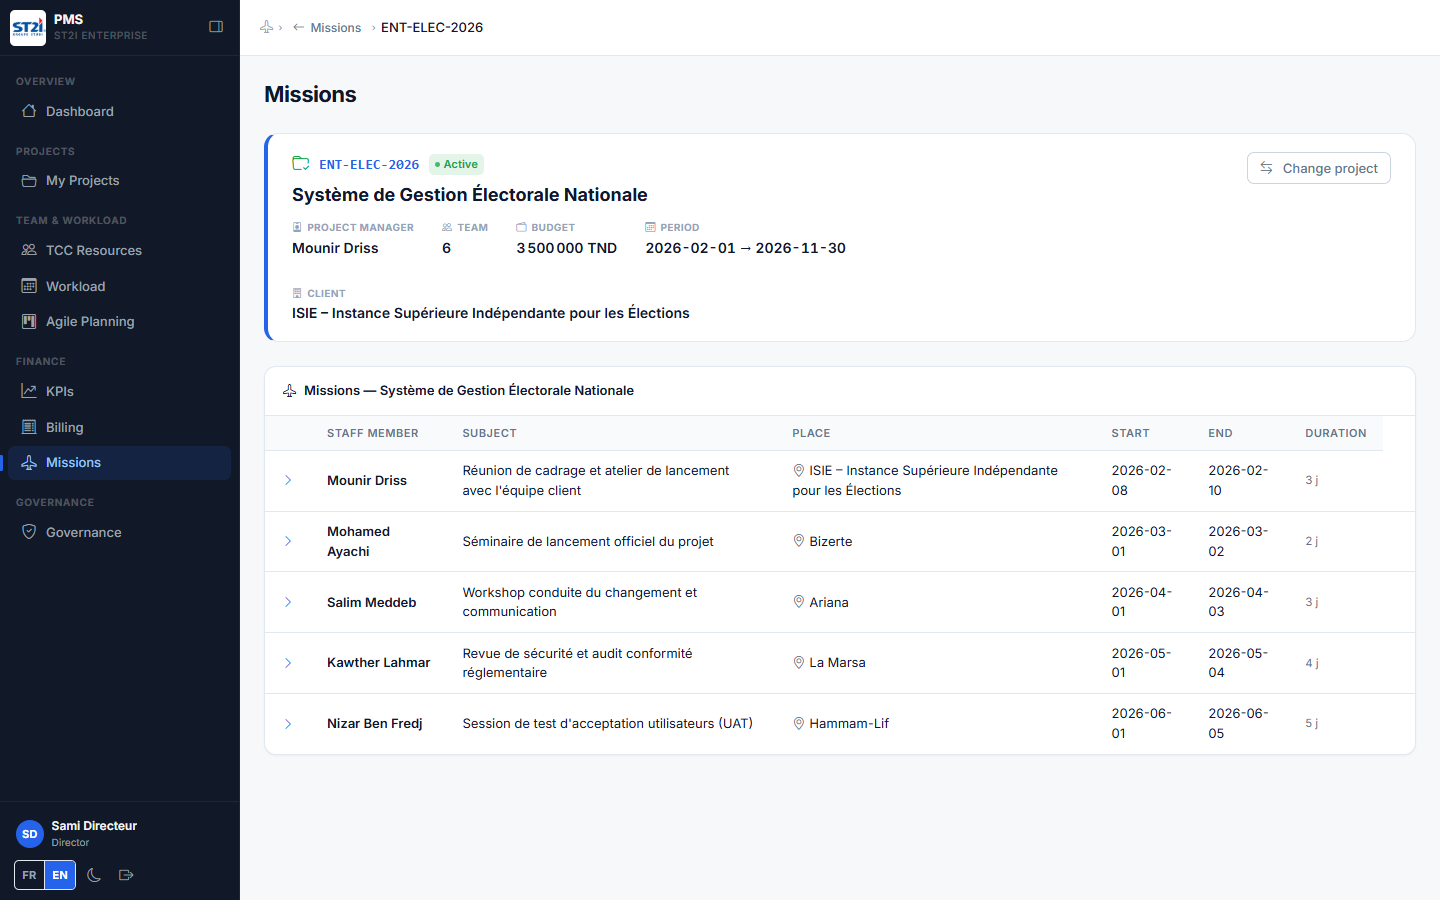
\includegraphics[width=0.95\columnwidth]{img/ui_missions.png}
  \caption{Missions interface, with the cost components of a mission expanded}
  \label{fig:ui-missions}
\end{figure}

\subsection{Testing}
The tests for this sprint sit with the module they check, and they run together with all the
others. They were run again for this report, and the counts below come from that run.

\textbf{\texttt{JalonServiceTest} (10 tests).} It checks the billing limit. A set of milestones
adding up to more than 100\% is refused, and one that adds up to exactly 100\% is accepted. It
then checks that a milestone already invoiced or paid cannot be invoiced again and cannot be
deleted. Last, it checks that the status is recomputed after a partial payment and after a full
one.

\textbf{\texttt{AvenantServiceTest} (5 tests).} It checks that the revised budget changes through
an amendment and in no other way.

\textbf{\texttt{BillingControllerTest} (8 tests).} It calls every endpoint of the module and
checks the permission each one requires.

That is 23 tests for this sprint, and all of them pass.

\subsection{Sprint review}
This review was the most literal of them all. The billing progress sheet of the workbook was
entered again, milestone by milestone, and the invoiced totals were compared line by line. The
limit on the sum of the percentages was checked first. The spreadsheet states that limit, but only
the platform enforces it.

% =====================================================================
\section{Sprint 7 --- Project governance}

\subsection{Sprint objectives}
Sprint~7 ran from 15~June to 3~July, three weeks (Table~\ref{tab:schedule}). Its objective is to
carry over the registers the workbook keeps beside the figures: risks, deliverables, stakeholders
and change requests. They are what makes a review a review rather than a balance sheet.

\subsection{Sprint backlog}
The sprint commits the following items of the product backlog (Table~\ref{tab:backlog}).

\begin{longtable}{|m{1.6cm}|m{12.4cm}|}
\caption{Sprint 7 backlog}\label{tab:sb7}\\
\hline
\textbf{Story} & \textbf{User story} \\
\hline
\endfirsthead
\hline
\textbf{Story} & \textbf{User story} \\
\hline
\endhead
\endfoot
\endlastfoot
\hline
US-24 & As a project manager, I want to keep a risk register \\
\hline
US-25 & As a project manager, I want to track deliverables and measure delivery progress \\
\hline
US-26 & As a project manager, I want to document the project stakeholders \\
\hline
US-27 & As a project manager, I want to record change requests \\
\hline
\end{longtable}

\subsection{Task planning}
The author being the sole developer, each item was expanded directly into the technical work it
required rather than distributed across a team.

\begin{longtable}{|m{1.6cm}|m{12.4cm}|}
\caption{Sprint 7 task planning}\label{tab:tp7}\\
\hline
\textbf{Story} & \textbf{Technical work} \\
\hline
\endfirsthead
\hline
\textbf{Story} & \textbf{Technical work} \\
\hline
\endhead
\endfoot
\endlastfoot
\hline
US-24 & Risk with probability, impact, status and mitigation plan \\
\hline
US-25 & Deliverable with a controlled status, feeding the delivery rate of the indicator engine \\
\hline
US-26 & Stakeholder register composed by the project, edited by the project manager \\
\hline
US-27 & Change request register composed by the project, each carrying a priority, a status and a decision date \\
\hline
\end{longtable}

\subsection{Design}
The sprint covers the four registers that document the qualitative life of a project: risks,
deliverables, stakeholders and change requests. The project manager maintains them; the director
consults them.

\begin{figure}[H]
  \centering
  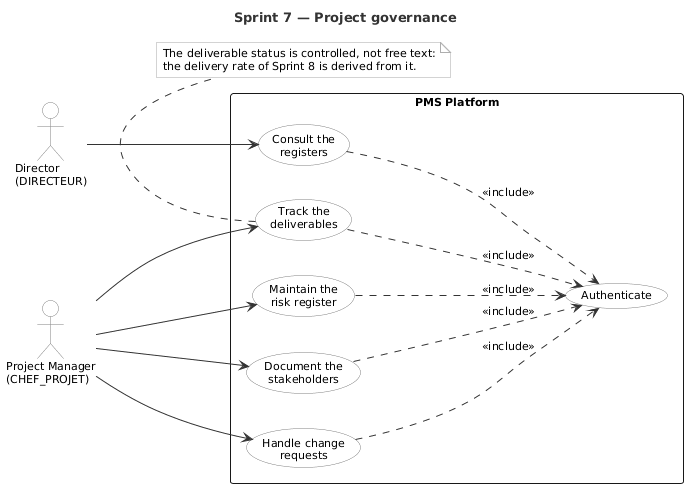
\includegraphics[width=0.75\columnwidth]{img/uc_sprint7.png}
  \caption{Use case diagram of sprint 7}
  \label{fig:uc-s7}
\end{figure}

\runin{Model of the governance registers}
The four registers share the same shape: each is composed by the project and governed by a small
business enumeration.

\begin{figure}[H]
  \centering
  
\includegraphics[width=0.95\columnwidth]{img/class_governance.png}
  \caption{Class diagram --- project governance}
  \label{fig:class-gov}
\end{figure}

\runin{Design decisions}
\textbf{The registers are attached to the project, not kept beside it.} Their value lies less in
their individual complexity than in belonging to the project itself, which the spreadsheet process
could not guarantee: risks and deliverables lived in separate documents that drifted from the
workbook.

\textbf{A deliverable carries a controlled status, not free text.} This is not documentation
tidiness. The delivery rate consumed by the indicator engine of Sprint~8 is derived from this
register, as the ratio of delivered and validated deliverables to planned ones. A free-text status
could not be counted, and the indicator would have had no input.

\textbf{Deletion is logical.} Removing an entry deactivates it and preserves the history, so that a
risk closed months ago remains visible in the record of how the project was steered.

\subsection{Implementation}
Each register exposes the same nested-resource shape under a project, with authorization carried by
the service layer and a dedicated pair of permissions separating consultation from modification.

\begin{figure}[H]
  \centering
  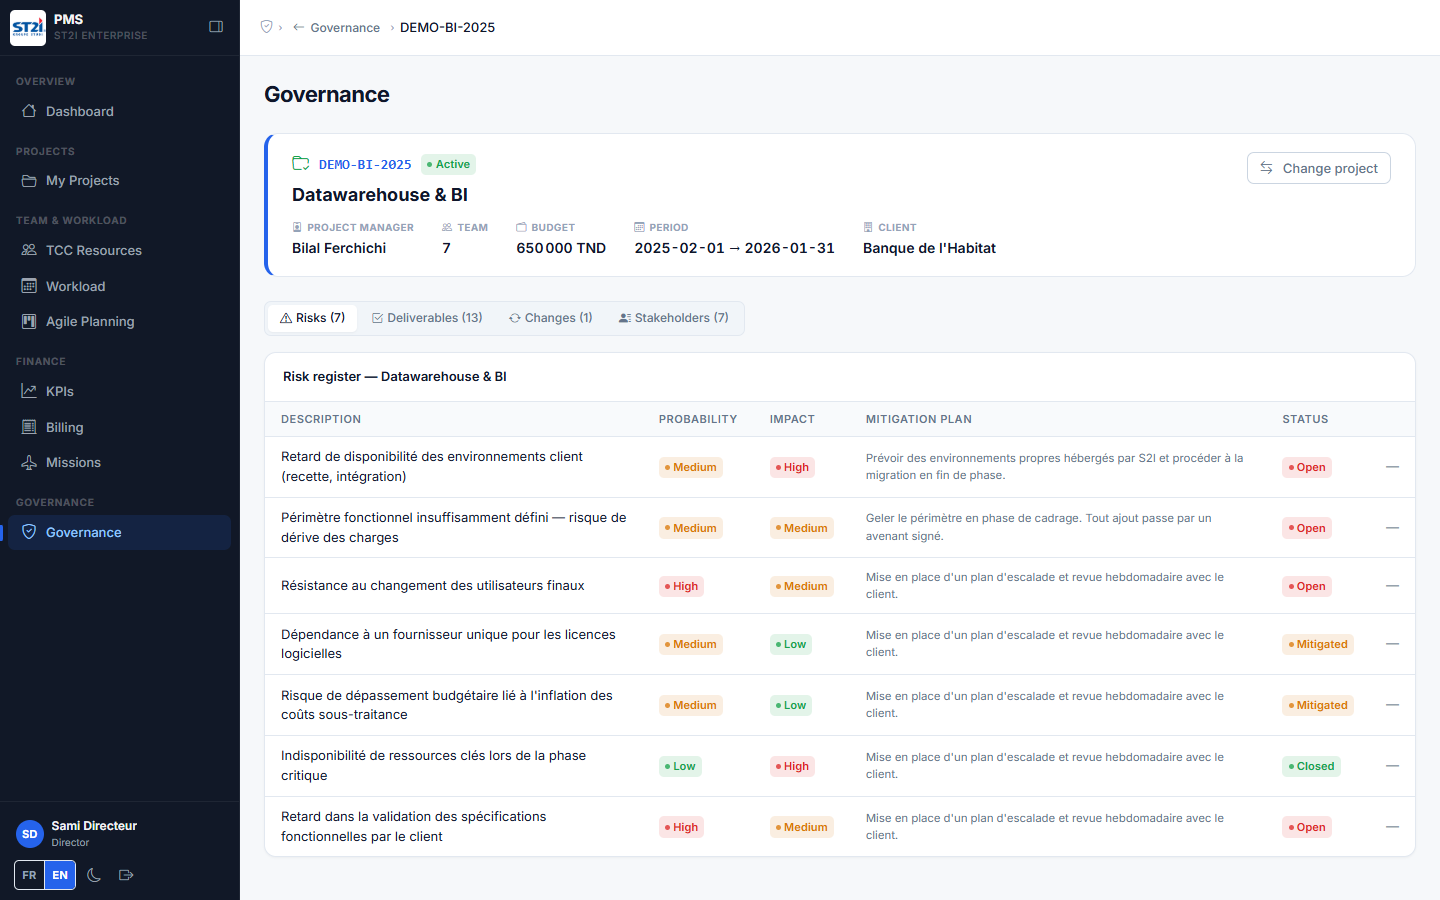
\includegraphics[width=0.95\columnwidth]{img/ui_governance.png}
  \caption{Governance interface}
  \label{fig:ui-gov}
\end{figure}

\subsection{Testing}
The tests for this sprint sit with the module they check, and they run together with all the
others. They were run again for this report, and the counts below come from that run.

\textbf{\texttt{GovernanceControllerTest} (8 tests).} It writes to each of the four registers and
reads them back, and checks the permission every endpoint requires.

All 8 of them pass.

\subsection{Sprint review}
The four registers were compared with the matching sheets of the workbook, field by field. One
point mattered more than the others. The status of a deliverable is chosen from a fixed list and
is not typed freely. The delivery rate of the next sprint reads that status, and free text would
have made the indicator impossible to compute.

% =====================================================================
\section{Sprint 8 --- Internal quote and indicator engine}

\subsection{Sprint objectives}
Sprint~8 ran from 6 to 24~July, three weeks (Table~\ref{tab:schedule}). Its objective is to close
the business scope with the part the whole project exists for: the economic baseline, and the
earned-value indicators the workbook computes by hand.

\subsection{Sprint backlog}
The sprint commits the following items of the product backlog (Table~\ref{tab:backlog}).

\begin{longtable}{|m{1.6cm}|m{12.4cm}|}
\caption{Sprint 8 backlog}\label{tab:sb8}\\
\hline
\textbf{Story} & \textbf{User story} \\
\hline
\endfirsthead
\hline
\textbf{Story} & \textbf{User story} \\
\hline
\endhead
\endfoot
\endlastfoot
\hline
US-28 & As a director, I want to give the project an economic baseline \\
\hline
US-29 & As a project manager, I want the financial indicators computed automatically \\
\hline
US-30 & As a project manager, I want to freeze a monthly review as history \\
\hline
US-31 & As a director, I want to supervise the whole portfolio \\
\hline
\end{longtable}

\subsection{Task planning}
The author being the sole developer, each item was expanded directly into the technical work it
required rather than distributed across a team.

\begin{longtable}{|m{1.6cm}|m{12.4cm}|}
\caption{Sprint 8 task planning}\label{tab:tp8}\\
\hline
\textbf{Story} & \textbf{Technical work} \\
\hline
\endfirsthead
\hline
\textbf{Story} & \textbf{Technical work} \\
\hline
\endhead
\endfoot
\endlastfoot
\hline
US-28 & Internal quote structured by section, gated by a dedicated permission \\
\hline
US-29 & Recompute-on-read engine valuing effort at the cost rate of its own year \\
\hline
US-30 & Immutable snapshot storing the indicators and the earned value entered by the manager \\
\hline
US-31 & Per-project and portfolio dashboards derived from the same engine \\
\hline
\end{longtable}

\subsection{Design}
The sprint covers the use cases that produce the figures the platform exists for: defining the
internal quote, consulting the computed indicators, freezing a monthly review, and consulting the
portfolio dashboard. The internal quote is reserved to the director alone.

\begin{figure}[H]
  \centering
  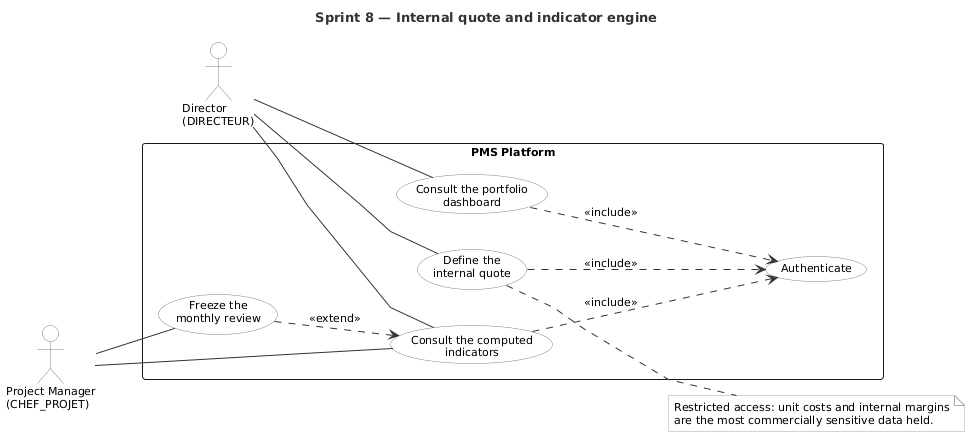
\includegraphics[width=0.75\columnwidth]{img/uc_sprint8.png}
  \caption{Use case diagram of sprint 8}
  \label{fig:uc-s8}
\end{figure}

\runin{Model of the indicator engine}
The engine reads from every module built since Release~1: workload for consumed and remaining
effort, cost rates for valuation, billing for invoiced revenue, and the deliverable register for
delivery progress.

\begin{figure}[H]
  \centering
  
\includegraphics[width=0.95\columnwidth]{img/class_kpi.png}
  \caption{Class diagram --- workload and indicator engine}
  \label{fig:class-kpi}
\end{figure}

\runin{Sequence from workload entry to frozen review}
Figure~\ref{fig:seq-kpi} shows the complete chain, from the submission of a month of effort to the
snapshot that freezes the monthly review.

\begin{figure}[H]
  \centering
  
\includegraphics[width=0.95\columnwidth]{img/seq_submit_workload.png}
  \caption{Sequence diagram --- workload entry and indicator computation}
  \label{fig:seq-kpi}
\end{figure}

\runin{Design decisions}
\textbf{Amounts and margins are never stored.} They are recomputed at read time from quantities,
unit values and the exchange rate. Persisting them would duplicate commercially sensitive figures
and allow the stored value to diverge from its inputs, which is exactly the failure the workbook
suffered when a formula was overwritten by a pasted constant.

\textbf{A read has no side effect.} Consulting a dashboard writes nothing. This is what makes the
indicators safe to display anywhere, and it is why two consecutive reads always agree.

\textbf{The earned value is entered, not computed.} The percentage of value earned is a judgement
made by the project manager during the monthly review, not a measurement the system can derive.
Pretending otherwise would have produced an indicator that looks objective and is not.

\textbf{The monthly review is frozen and immutable.} Submitting the review creates a snapshot of the
indicators of that month. This is the digital equivalent of the monthly column of the statistics
sheet: live figures for steering, frozen figures for history. A later correction cannot rewrite a
review a decision was already based on.

\textbf{The internal quote is gated by its own permission.} Unit costs and internal margins are the
most commercially sensitive data the platform holds, so access is not inherited from the project
role but granted explicitly and separately.

\subsection{Implementation}
The sprint delivers the baseline a project is measured against, and the engine that measures it.


\runin{The internal quote}
The quote is the economic baseline of the project: line items grouped by section, each carrying a
sold quantity and unit price on the revenue side, and an internal quantity and unit cost on the cost
side. The computation runs in two passes so that section subtotals and the overall margin remain
consistent with the line items they summarise.

\runin{The computed indicators}
On each read the engine recomputes, from live data, the indicators of the reference workbook:

\begin{itemize}
  \item \textbf{Actual cost} --- consumed man-days valued at the cost rate of their own year;
  \item \textbf{ETC} --- remaining man-days valued the same way;
  \item \textbf{EAC} --- actual cost plus ETC;
  \item \textbf{Production revenue} --- contract total weighted by the earned value percentage;
  \item \textbf{Accrued income} --- production revenue minus the invoiced total;
  \item \textbf{Margin} --- effective budget minus EAC, in value and in percentage;
  \item \textbf{Drift} --- sold workload minus consumed minus remaining.
\end{itemize}

Figure~\ref{fig:ui-kpi} shows them as the project manager reads them, each indicator
beside the value it is computed from.

\begin{figure}[H]
  \centering
  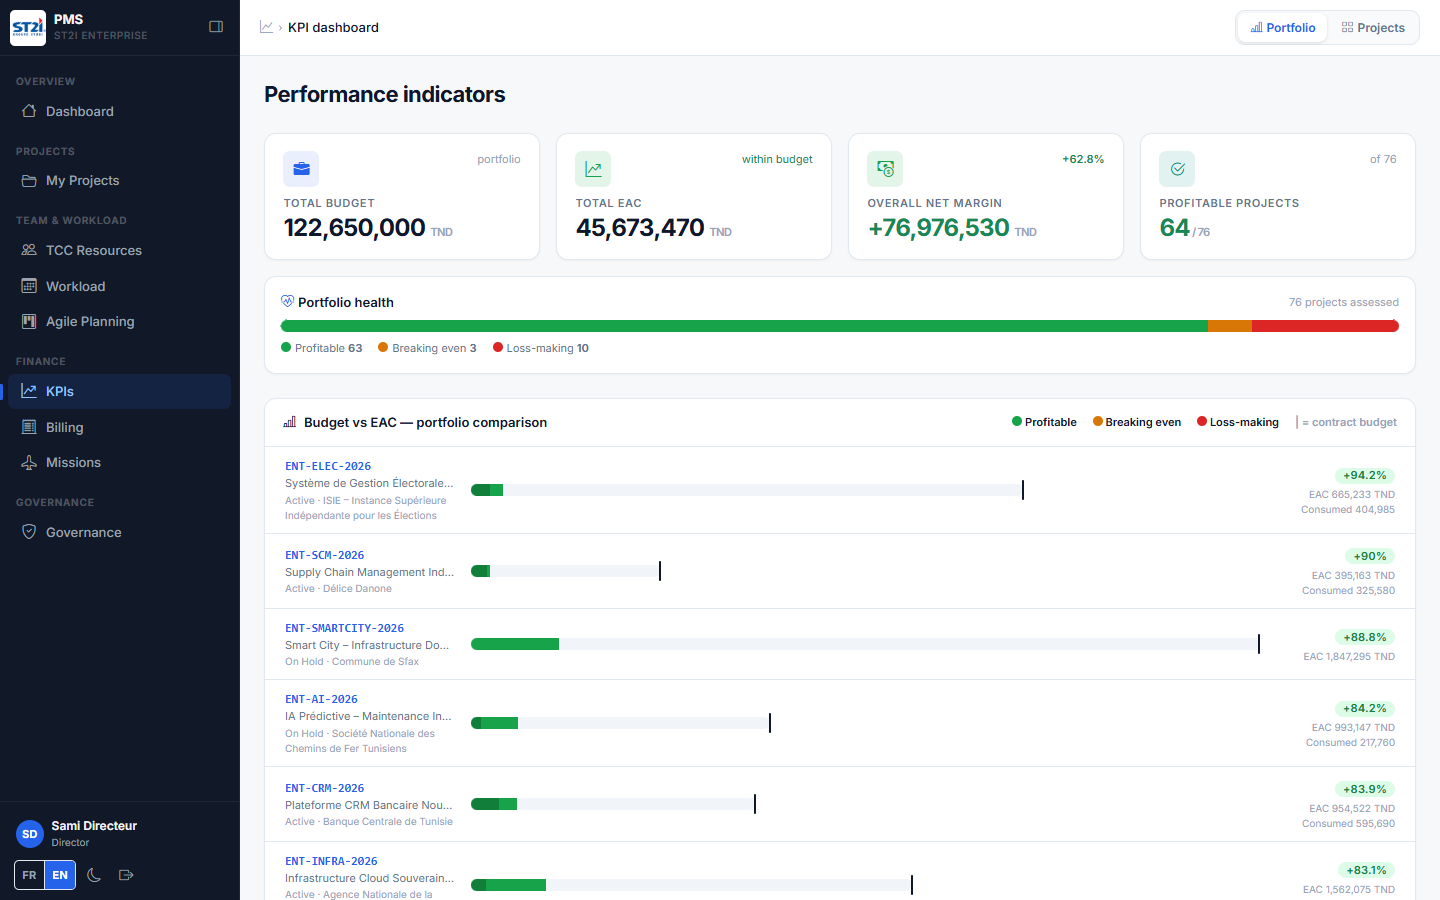
\includegraphics[width=0.95\columnwidth]{img/ui_kpi.png}
  \caption{KPI dashboard interface}
  \label{fig:ui-kpi}
\end{figure}

The same engine feeds the portfolio view of the director, which ranks every project by margin and
summarises the health of the whole portfolio in one bar. This is the screen that replaces the
manual consolidation the company had no way to automate: one workbook per project could be read
one at a time, never together.

\begin{figure}[H]
  \centering
  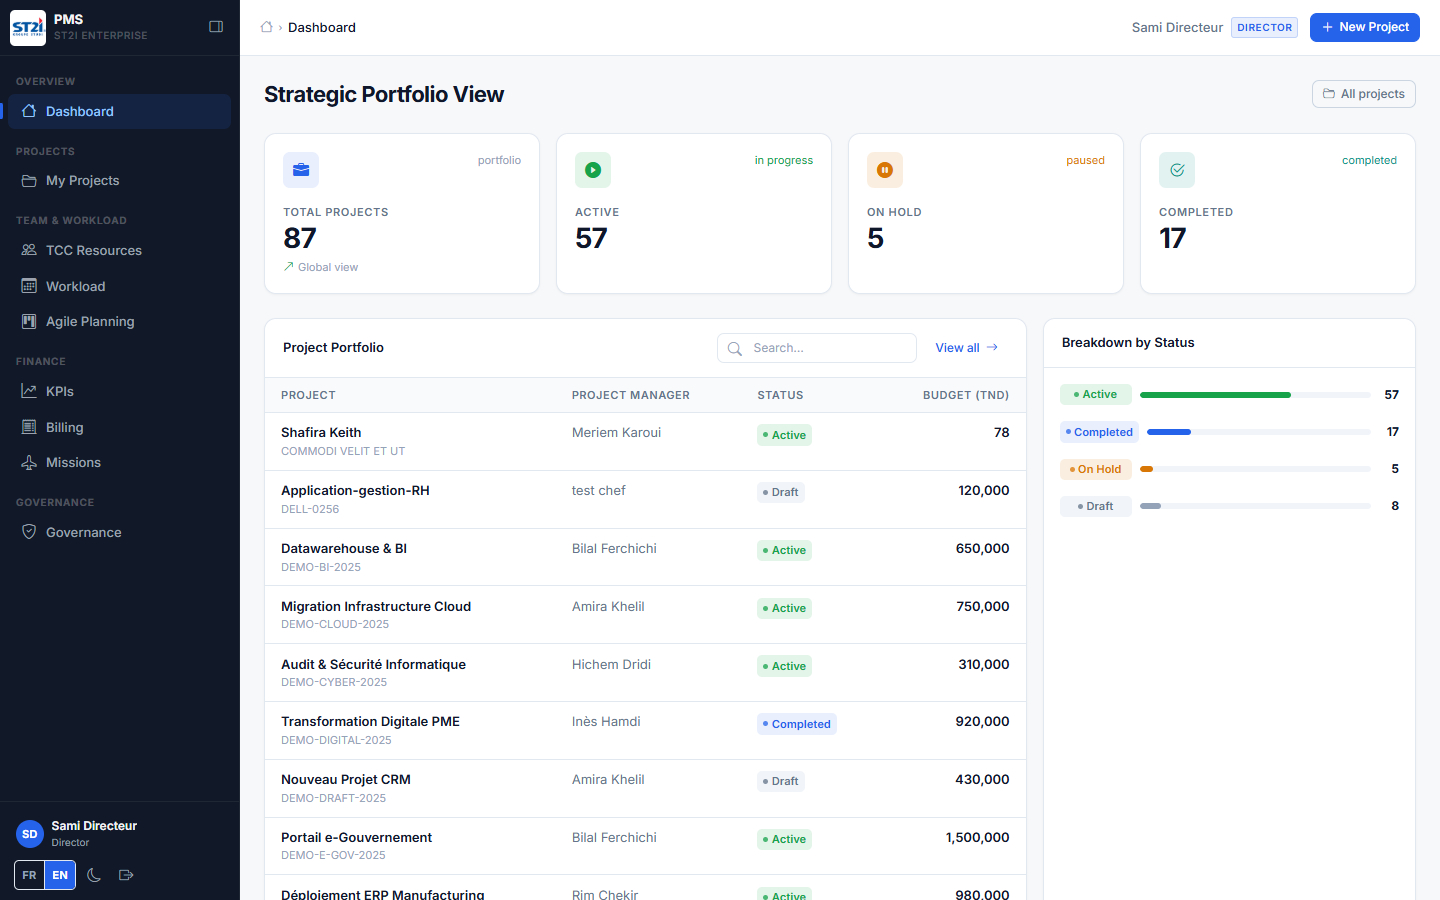
\includegraphics[width=0.95\columnwidth]{img/ui_dashboard.png}
  \caption{Portfolio dashboard of the director}
  \label{fig:ui-portfolio}
\end{figure}

\subsection{Testing}
The tests for this sprint sit with the module they check, and they run together with all the
others. They were run again for this report, and the counts below come from that run.

\textbf{\texttt{DevisInterneServiceTest} (4 tests).} It checks that the internal quote can be
reached only with its own permission.

\textbf{\texttt{KpiControllerTest} (6 tests).} It reads the indicators and the dashboards, and
checks that only the roles allowed to see financial data can reach them.

That is 10 tests for this sprint, and all of them pass.

\subsection{Sprint review}
The review was a direct comparison. One project was entered on the platform, then the indicators
were read twice: once in the workbook, once on the dashboard. Where the two figures differed, the
workbook was treated as correct and the engine was corrected. The workbook is the real
specification of the company.

% =====================================================================
\section*{Conclusion}
\addcontentsline{toc}{section}{Conclusion}
Release~3 delivered what PMS was commissioned for: billing and expenses, the governance registers,
the internal quote, and above all the indicator engine that replaces the two thousand formulas of
the reference workbook. The engine works in two ways. It computes live figures for steering, and
it freezes snapshots for history. This keeps what the spreadsheet did well and removes what made
it fragile.

        \clearpage

        \chapter{Release 4 --- Consolidation, Delivery and Deployment}

\section*{Introduction}
The functional scope of the platform was completed at the end of Release~3. This final release makes
it deliverable: a coherent and accessible user interface, a verified authorization policy, a
security review, and a reproducible deployment. It gathers two sprints: Sprint~8 consolidates the interface and
verifies the platform, Sprint~9 makes it reproducibly deployable and continuously verified.
Neither delivers new business functionality; both deliver deliverability.

% =====================================================================
\section{Sprint 8 --- Interface Consolidation, Testing and Deployment}

\subsection{Sprint Objective}
Bring the platform to a deliverable state: unify the user interface, verify that the security model
behaves as designed, review the application against the common web vulnerabilities, and package it
for deployment.

\subsection{Functional Scope}
This sprint covers user story US-26, a consistent and responsive interface, and the
cross-cutting quality work that no single functional story carries.

\subsection{Features Implemented}
\begin{itemize}
  \item Frontend application structure and session handling.
  \item Authorization model applied to the interface.
  \item Design system unifying the screens of the eight modules.
  \item Automated test suite covering the business rules and the access control.
  \item Security review against the common web vulnerabilities.
  \item Deployment packaging.
\end{itemize}

\subsection{Technical Realisation}

\subsubsection{Frontend structure and session handling}
The client is a single-page application organised by feature, mirroring the backend modules. The
access token obtained at sign-in is kept in memory and attached to every request by an HTTP
interceptor; the refresh token remains in its \texttt{HttpOnly} cookie, unreachable from
JavaScript. When a request returns \texttt{401}, the interceptor attempts a single refresh before
returning the user to the sign-in screen.

\subsubsection{Authorization applied to the interface}
The interface consumes the permission list returned by \texttt{GET /api/me/context} and derives
from it both the navigation menu and the visibility of individual actions. A button that the user
is not entitled to use is not merely disabled: it is absent.

This must be understood correctly, and the report states it explicitly: hiding a control is an
\textbf{ergonomic} measure, not a security measure. The authorization decision is taken by the
server on every request, as described in Sprint~2. The client-side rule exists so that the user is
never offered an action that would be refused; it is never the thing that refuses it.

\subsubsection{Design system and interface consolidation}
The eight modules were built successively, each with its own screens. This sprint unified them
behind a single design system: a token-based visual language (colours, typography, spacing,
elevation) declared once and consumed by every screen, together with a set of shared components
(pagination, selection, confirmation dialog, notifications) reused across the modules rather than
reimplemented in each.

The consolidation also addressed accessibility and consistency: sortable table headers announcing
their state, labelled icon-only controls, explicit empty states in place of blank tables, and a
responsive layout. The interface being the only part of the platform its users ever see, this
convergence matters as much to adoption as the correctness of the engine behind it.

\subsubsection{Test strategy}
Testing concentrates on what a regression would make expensive: the business rules and the
authorization model. The automated backend suite covers the lifecycle transitions, the billing
ceiling, workload uniqueness and immutability, the multi-currency conversions, and the indicator
formulas compared against the reference workbook.

The access control receives dedicated attention: for each protected endpoint, the suite verifies
that a caller holding the permission succeeds and that a caller without it is refused. This is what
makes the ``configurable authorization'' claim verifiable rather than merely stated.

\subsubsection{Security review}
The application was reviewed against the common categories of web vulnerability:

\begin{longtable}{|m{4.6cm}|m{10cm}|}
\hline
\textbf{Category} & \textbf{Measure taken} \\
\hline
\endhead
\endfoot
\endlastfoot
\hline
Broken access control & Every endpoint annotated with its required permission; scope checked
independently of permission; no role name tested in code \\
\hline
Cryptographic failures & Passwords hashed with BCrypt; tokens signed; refresh token confined to an
\texttt{HttpOnly}, \texttt{Secure}, \texttt{SameSite} cookie \\
\hline
Injection & Parameterised queries through the ORM; no string-built SQL \\
\hline
Identification and session failures & Short-lived access token; instant revocation by token
version; forced password change on first login \\
\hline
Sensitive data exposure & Financial data filtered by permission; internal quote behind a dedicated
permission; computed amounts never persisted \\
\hline
Security misconfiguration & Schema managed by versioned migrations with the ORM in validation
mode; secrets externalised as environment variables \\
\hline
\caption{Security review by vulnerability category}
\label{tab:owasp}
\end{longtable}

\subsubsection{Packaging}
At the close of this sprint the platform is packaged as an executable archive for the backend and a
static build for the frontend, with the database schema brought up to date by the migration tool at
startup and all configuration supplied by environment variables.

Startup is idempotent: deploying the same artefact against an up-to-date database changes nothing,
and against an older one applies exactly the missing migrations.

This packaging is sufficient to run the application, but not to \emph{deploy} it reproducibly:
it still assumes a host on which the right Java version, the right Node version and a correctly
provisioned PostgreSQL instance are already present. Sprint~9 removes that assumption.

\subsection{Tests and Validation}

\begin{longtable}{|m{4.2cm}|m{5.4cm}|m{4.8cm}|}
\hline
\textbf{Test case} & \textbf{Steps} & \textbf{Expected result} \\
\hline
\endhead
\endfoot
\endlastfoot
\hline
Business rule suite & Run the automated backend tests & All pass \\
\hline
Permission granted & Call each protected endpoint with the permission & Operation performed \\
\hline
Permission missing & Call each protected endpoint without it & HTTP 403 \\
\hline
Financial confidentiality & Browse the interface as a developer & No financial figure exposed \\
\hline
Menu consistency & Sign in with each of the four roles & Each menu matches the permissions held \\
\hline
Deployment & Start the artefact against an empty and an existing database & Schema created, then
migrated without loss \\
\hline
\caption{Test cases --- Sprint 8}
\label{tab:tests-s8}
\end{longtable}

\subsection{Sprint Outcome}
The platform is functionally complete, verified on its business rules and its authorization model,
reviewed for the common vulnerabilities, and packaged as a runnable artefact.

\subsection{Transition to the Next Sprint}
One gap remains between ``it runs on my machine'' and ``it can be deployed'': the artefact still
depends on a correctly prepared host. Sprint~9 closes that gap with containerization and a
continuous integration pipeline.

% =====================================================================
\section{Sprint 9 --- Containerization and Continuous Delivery}

\subsection{Sprint Objective}
Make the platform reproducibly deployable and continuously verified: package each component as a
container image, orchestrate the whole stack with a single command, and automate build, test and
integration checks on every change.

\subsection{Functional Scope}
This sprint delivers no new business functionality. Its scope is the delivery chain itself, and it
addresses an item already open in the project's engineering backlog: the absence of deployment
documentation and of any reproducible deployment procedure.

\subsection{Features Implemented}
\begin{itemize}
  \item Container image for the backend, built in two stages and running as a non-root user.
  \item Container image for the frontend, serving the production build and reverse-proxying the API.
  \item Orchestration of the three services with health checks and startup ordering.
  \item Continuous integration pipeline: build, tests, image construction, end-to-end smoke test.
  \item Deployment documentation and an architecture decision record superseding the previous one.
\end{itemize}

\subsection{Technical Realisation}

\subsubsection{A reconsidered architecture decision}
The project had initially recorded a decision to run natively, without containers, justified by
iteration speed on an already-provisioned machine. That decision served development well but left
two gaps: no reproducible deployment, and a production profile that had never actually been
executed.

The decision was therefore superseded rather than silently contradicted: a new record documents the
move to containers, states what it changes, and confirms what it does \emph{not} change. In
particular, three containers are \textbf{not} three microservices: the modular monolith decision
stands. What is containerized is one application, its database and its static server.

\subsubsection{Image construction}
Both images are built in two stages, so that the build toolchain never reaches the runtime image:
the backend image contains a Java runtime and the application archive, with neither Maven nor
sources; the frontend image contains a web server and the compiled assets, with no Node runtime.
The backend container runs as a dedicated unprivileged user rather than as root.

Tests are deliberately \textbf{not} executed during image construction. Building an image is a
packaging step; the quality gate belongs to the pipeline. Running the suite in both places would
double build time without producing any additional signal.

\subsubsection{Single origin through the reverse proxy}
The web server serves the application and forwards \texttt{/api} to the backend container. The
browser therefore contacts a single origin, which has a concrete consequence: the cross-origin
configuration required by the development setup becomes unnecessary, and the refresh cookie,
restricted to its own path and marked \texttt{SameSite=Strict}, works without any exception.
The containerized deployment is, on this point, simpler and safer than the development loop.

\subsubsection{Startup ordering and health probes}
Composing three services raises an ordering problem: a container being \emph{started} is not the
same as a container being \emph{ready}. The stack therefore relies on health probes rather than on
declaration order. The database is probed over TCP, because the temporary server used during
initialisation accepts only local socket connections and would otherwise be reported ready too
early. The backend exposes a health endpoint, deliberately left unauthenticated but returning no
detail, and is given a generous startup window because its first run applies the full set of
schema migrations, including the demonstration dataset.

\subsubsection{Defects revealed by the exercise}
Preparing the pipeline exposed three pre-existing defects that native execution had concealed. The
most consequential concerned the frontend build configuration: the production configuration never
substituted the production environment file, so the production bundle embedded the development API
address. On the development machine the application appeared to work, because the bundle was calling the
local backend, while it would have been broken on any other host. The second was a build wrapper
documented in the project files but absent from the repository. The third was an ignore rule that
silently excluded the configuration template from version control, precisely the file the
deployment procedure requires.

That these defects surfaced only when the delivery chain was automated is itself the argument for
automating it.

\subsubsection{Pipeline}
The pipeline separates what must always hold from what is only meaningful on integration branches.
Compilation, the backend test suite, the production frontend build and the construction of both
images run on every proposed change: a component that only breaks after merging is not a gate. The
end-to-end test, which starts the full stack and performs a real authentication through the
reverse proxy, runs on integration branches, where its cost is justified. Image publication is
reserved for the main branch.

The frontend job also carries an explicit guard against the defect described above: it fails if the
development address reappears in the production bundle.

\subsection{Tests and Validation}

\begin{longtable}{|m{4.2cm}|m{5.4cm}|m{4.8cm}|}
\hline
\textbf{Test case} & \textbf{Steps} & \textbf{Expected result} \\
\hline
\endhead
\endfoot
\endlastfoot
\hline
Environment substitution & Inspect the production bundle & The development address is absent \\
\hline
Unprivileged execution & Inspect the identity inside the backend container & Non-root user \\
\hline
Full stack startup & Start the three services & All three reported healthy \\
\hline
Schema migration & Count the applied migrations on a pristine volume & All migrations applied \\
\hline
End-to-end authentication & Authenticate through the reverse proxy & Token returned and refresh
cookie set \\
\hline
Client-side routing & Reload a deep application route & The application is served, not a 404 \\
\hline
Persistence & Stop and restart the stack & Data preserved; a volume reset replays the migrations \\
\hline
Development loop & Run the native backend and frontend while the stack is up & Both coexist, no
port collision \\
\hline
\caption{Test cases --- Sprint 9}
\label{tab:tests-s9}
\end{longtable}

\subsection{Sprint Outcome}
The platform is deployable by a single command on any machine running a container engine, and every
change is now verified automatically. The deployment procedure, the environment variables, the
backup method and the known pitfalls are documented.

\subsection{Final State of the Product}
At the end of the nine sprints, PMS covers the whole scope identified during the analysis of the
Excel workbook: dynamic authorization, project and team management, workload planning and
recording, billing, missions, governance and the earned-value indicator engine, all behind a
unified interface. Table~\ref{tab:final} summarises the path from the reference workbook to the
delivered platform.

\begin{longtable}{|m{2.0cm}|m{5.6cm}|m{6.8cm}|}
\hline
\textbf{Sprint} & \textbf{Increment delivered} & \textbf{Excel logic replaced} \\
\hline
\endhead
\endfoot
\endlastfoot
\hline
Sprint 1 & Technical foundation, authentication & --- (no spreadsheet equivalent) \\
\hline
Sprint 2 & Dynamic authorization, users, resources, cost rates & TCC sheet \\
\hline
Sprint 3 & Projects and lifecycle & Identification sheet \\
\hline
Sprint 4 & Teams, workload plan and actuals & Forecast cost and actual cost sheets \\
\hline
Sprint 5 & Billing, payments, amendments, missions & Billing progress and missions sheets \\
\hline
Sprint 6 & Governance registers & Risks, deliverables, stakeholders, changes sheets \\
\hline
Sprint 7 & Internal quote and indicator engine & Statistics and dashboard sheets \\
\hline
Sprint 8 & Interface consolidation, tests, security review & --- (quality) \\
\hline
Sprint 9 & Containerization and continuous delivery & --- (delivery chain) \\
\hline
\caption{From the reference workbook to the delivered platform}
\label{tab:final}
\end{longtable}

\section*{Conclusion}
Release~4 closed the construction of the platform by addressing what functionality alone does not
deliver: a coherent interface, a verified security model and a reproducible deployment. The
incremental path followed since Release~1 (foundation, operations, finance, consolidation)
produced a platform whose every increment was demonstrable in isolation, and whose final state
covers the entire business logic previously carried by the Excel workbook.

        \clearpage


        \chapter*{General Conclusion and Perspectives}
\addcontentsline{toc}{chapter}{General Conclusion and Perspectives}
\markboth{General Conclusion}{General Conclusion}

The objective of this final year project was to replace a scattered, spreadsheet-based project
steering process with a centralised platform that preserves the richness of the existing financial
model while removing its fragility. That objective is met: PMS covers the whole functional scope
identified during the analysis of the reference workbook, from dynamic authorization to the
earned-value indicator engine.

\section*{Assessment}
The construction proceeded through ten increments, each demonstrable in isolation. Release~1
delivered the technical foundation, authentication and above all the dynamic authorization model.
Release~2 opened operational steering with projects, teams and workload. Release~3 delivered the
core business value: billing, missions, governance and the indicator engine. Release~4
consolidated the interface, verified the security model, and made the platform reproducibly
deployable through containerization and a continuous integration pipeline.

Three design decisions structure the result and are, in retrospect, the ones that mattered most.

The first is the \textbf{dynamic authorization model}. By inserting a permission level between
roles and modules, and by keeping the role--permission matrix in the database, the platform makes
its security policy configurable data rather than compiled code. Granting a new right is an
administrative act, not a release.

The second is the \textbf{hybrid indicator engine}. Rather than choosing between recomputing
indicators on demand and persisting them, the platform does both: live computation guarantees that
no dashboard displays a stale figure, while a frozen monthly snapshot preserves the official state
of each review. This reproduces the strength of the original workbook, a live dashboard with monthly
history, without its fragility.

The third is the \textbf{normalisation of the monthly time series}. Replacing a grid of month
columns with one row per project, resource and month turned a structural limitation of the
spreadsheet into a simple insertion, and made integrity constraints expressible: no duplicate
month, no entry on an unassigned project, no silent rewriting of a validated period.

\section*{Skills Acquired}
Beyond the technologies used, this project required reading a real business model out of an
artefact that was never written as a specification, and arbitrating between what the workbook did,
what the written specifications said, and what the code could reasonably guarantee. It also
required designing for confidentiality: deciding that commercially sensitive amounts should be
computed on read rather than stored is an engineering decision with a business justification, not a
technical preference.

\section*{Limitations and Perspectives}
Several avenues remain open.

\textbf{Automatic time-tracking import.} The workload model was designed to accept a second data
source alongside manual entry, so that effort recorded in an external time-tracking tool could be
imported and reconciled. The mechanism is anticipated in the design but not implemented; it is the
most immediate extension.

\textbf{Reporting and export.} The platform computes and displays the indicators; generating
exportable review documents in the format the company already circulates would shorten the last
manual step of the monthly review.

\textbf{Integration with the information system.} The business rules explicitly anticipate future
integration points with accounting, human resources and enterprise systems. The modular
organisation of the code was chosen with that reversibility in mind: a module can be extracted
behind an interface without restructuring the whole.

\textbf{Scaling the deployment.} The current deployment targets the internal use of one company. A
significant growth in the number of projects or users would justify revisiting the modular monolith,
a decision deliberately taken as reversible rather than permanent.

The platform delivered is therefore both an answer to an immediate operational need and a
foundation on which the company's project steering can continue to evolve.

        \clearpage
        
        % @author: Stoufa
		% the command `\nocite{*}` is mandatory to avoid the “no \citation commands” error
        % https://tex.stackexchange.com/questions/18045/problem-with-compiling-bibtex-no-citation-commands-error
        \nocite{*}
        
%          \input{webo}
%         \clearpage
        
        % Every source is a web page, not a book: the school's own reports head
        % this list "Webography" rather than "Bibliography".
        \printbibliography[title={Webography},heading=bibintoc]
        
       
        
        % \input{annexes}
        % \clearpage

    \backmatter
        \input{./tpl/resume}
    
\end{document}